\documentclass[10pt,a4paper]{article}
\usepackage{amsmath,amssymb,graphicx,booktabs,hyperref}
\hypersetup{hidelinks}
% Journal formatting requirements: double line spacing and continuous line numbers.
% Enabled for the submission build via \def\REVIEWCOPY{} before \documentclass[10pt,a4paper]{article}
\usepackage{amsmath,amssymb,graphicx,booktabs,hyperref}
\hypersetup{hidelinks}
% Journal formatting requirements: double line spacing and continuous line numbers.
% Enabled for the submission build via \def\REVIEWCOPY{} before \documentclass[10pt,a4paper]{article}
\usepackage{amsmath,amssymb,graphicx,booktabs,hyperref}
\hypersetup{hidelinks}
% Journal formatting requirements: double line spacing and continuous line numbers.
% Enabled for the submission build via \def\REVIEWCOPY{} before \documentclass[10pt,a4paper]{article}
\usepackage{amsmath,amssymb,graphicx,booktabs,hyperref}
\hypersetup{hidelinks}
% Journal formatting requirements: double line spacing and continuous line numbers.
% Enabled for the submission build via \def\REVIEWCOPY{} before \input{main.tex};
% the compact reading version omits it.
\usepackage{setspace}
\renewcommand{\rmdefault}{ptm}
\renewcommand{\sfdefault}{phv}
\renewcommand{\ttdefault}{phv}
\input{fonts.tex}
\DeclareMathSizes{12}{10}{7}{5}
\DeclareMathSizes{9}{10}{7}{5}
\makeatletter\renewcommand\normalsize{\@setfontsize\normalsize{12}{15}}\makeatother
\normalsize
\setlength{\textwidth}{166mm}
\setlength{\textheight}{242mm}
\setlength{\oddsidemargin}{-3mm}
\setlength{\evensidemargin}{-3mm}
\setlength{\topmargin}{-15mm}
\setlength{\parskip}{3pt}
\setlength{\parindent}{12pt}
\setlength{\emergencystretch}{2em}
\renewcommand{\baselinestretch}{1.09}
\ifdefined\REVIEWCOPY\usepackage{lineno}\AtBeginDocument{\doublespacing\linenumbers}\fi
\renewcommand{\topfraction}{0.92}\renewcommand{\bottomfraction}{0.85}
\renewcommand{\textfraction}{0.06}\renewcommand{\floatpagefraction}{0.78}
\title{Auditing selective release of chest radiograph findings: retrospective evaluation of CC-Arbiter}
\author{Yaocong Yang and Xiangyong Kong\\[4pt]
\small School of Health Science and Engineering,\\
\small University of Shanghai for Science and Technology, Shanghai, China\\
\small Correspondence: Xiangyong Kong, \texttt{kxy@usst.edu.cn}}
\date{}
\begin{document}
\maketitle
\begin{abstract}
\noindent\textbf{Background:} Low error among selectively released chest radiograph findings can conceal the rejection of nearly all positive findings. We evaluated an executable evidence gate and audited its release, positive retention and failure boundaries.\par
\noindent\textbf{Methods:} CC-Arbiter intersects class-conditional conformal sets from two frozen DenseNet-121 experts and applies independently calibrated conditional-error gates using exact, multiplicity-corrected binomial bounds. The original cohorts comprised 2,116 NIH patients and 2,955 IU reports, with disjoint conformal, risk-calibration and test splits. Seven dataset annotations served as targets, without new clinical adjudication. A secondary protocol added calibration-only threshold baselines, score discrimination and comparisons at matched release counts. Frozen policies were then evaluated in 1,582 additional NIH patients absent from the original cohort. A separate review-routing study used 2,557 additional NIH patients, split into independent risk-calibration and test sets. It constrained both missed positives and positivity among unflagged patients. Projection-stratified results were examined post hoc. Score corruption and graph execution were also assessed.\par
\noindent\textbf{Results:} At the 10\% risk target, CC-Arbiter released 407/4,452 original NIH opportunities (9.1\%), with 10 errors (2.5\%; unit-bootstrap 95\% confidence interval, 1.1--4.1\%) and only 3/232 positive targets recovered. Positive predictive value was 27.3\%. It released nothing on IU. New-patient replication yielded 1,195/11,074 releases (10.8\%), 23 errors (1.9\%; 95\% confidence interval, 1.1--2.8\%), 8/507 positive targets recovered and positive predictive value of 30.8\%. Anteroposterior examinations received fewer and more erroneous releases than posteroanterior ones (originally 2.6\% versus 12.8\% release; 16.7\% versus 0.8\% error). Simple mean-score ranking at identical per-label release counts produced fewer errors in both NIH cohorts (5 and 14), while recovering fewer positives (0 and 3). Calibration-only Youden thresholds reduced IU mean-score error from 77.3\% to 29.9\%. Shared corruption in 61/636 original NIH patients raised CC-Arbiter error to 17.2\%. Both routing procedures flagged all 1,279 new test patients because no threshold met both constraints. All 43,470 original and replication label decisions matched offline gating.\par
\noindent\textbf{Conclusions:} The framework makes risk calibration and output enforcement auditable, but low selective error did not establish useful positive retention or superiority over simpler selection. Replication supports joint reporting of release, positive recall, matched-budget comparisons and correlated failures.
\end{abstract}
\noindent\textbf{Keywords:} chest radiograph; selective prediction; conformal prediction; risk control; medical imaging agents; reproducibility

\section{Background}
Medical imaging agents combine a planning model with specialist tools for image classification, visual question answering, segmentation and report generation. MedRAX introduced a unified chest radiograph tool interface and the ChestAgentBench benchmark~\cite{medrax}. CXRAgent and RadAgents further develop staged verification and radiologist-inspired workflows~\cite{cxragent,radagents}. These systems motivate a practical engineering question: which tool-derived statements may reach the user when experts disagree or provide uncertain evidence? Providing confidence information to a language model and enforcing an output rule are different operations. A model may disregard an uncertainty annotation, and a correctly written monitor may still be absent from the executed graph.

Conformal prediction provides one component of a solution. Given suitable calibration data and exchangeability, it constructs prediction sets with finite-sample coverage~\cite{vovk,gentle}. Coverage concerns whether a set contains the specified target; it does not by itself bound error among the subset of outputs that a system chooses to release. Intersecting multiple sets, selecting a singleton and withholding some predictions introduce further selection. A separate selective-risk argument is therefore needed. Moreover, a guarantee against imperfect dataset annotations does not become a guarantee against clinical diagnoses.

Risk calibration methods address several different objectives. Learn Then Test calibrates predictive procedures through hypothesis testing~\cite{ltt}. Conformal Risk Control addresses expected bounded losses under its assumptions~\cite{crc}; a joint wrong-and-released loss is not the conditional error among released predictions. SCoRE studies selective risk more directly~\cite{score}. Work on conformal model aggregation also shows that combining prediction sets requires its own analysis~\cite{coma}. Our aim is not to introduce a new conformal theorem. We implement a transparent finite-family procedure whose statistical unit, release rule and software execution can all be checked.

The resulting system, CC-Arbiter, operates on two classifier outputs for the same image or study and finding. It constructs a proposal from intersected conformal sets, calibrates whether that proposal can be released, and replaces the planner's final prose with a structured release-or-defer decision. We evaluate three questions: whether the final gate executes as specified; how much evidence remains after conditional-risk calibration; and whether low overall error is accompanied by useful positive findings or robustness to shared expert failures. The contribution is an auditable implementation and empirical assessment of these questions, including cases where the gate cannot certify useful output.

\section{Methods}
\subsection{Study design and annotation targets}
This retrospective computational study used NIH ChestX-ray14 and IU chest radiograph data~\cite{nih,iu}. The original analysis specification, threshold grid and split manifest were fixed before revised image-model inference and evaluation. This was an internal analysis lock, not public preregistration or a prospectively collected clinical cohort. The pretrained image experts were not fitted on either evaluation dataset. A later, separately specified review-routing extension fits a small score-combination model on original calibration patients only. The primary estimand is error with respect to seven specified dataset annotations: atelectasis, cardiomegaly, consolidation, edema, effusion, pneumonia and pneumothorax.

For NIH, both complete local parquet shards contained 2,458 image records from 2,116 patients. One image per patient was selected using the lexicographically smallest SHA-256 digest of its encoded image bytes, independently of labels and predictions. The resulting 2,116 units contain no duplicated selected image across patient identifiers. We used the released text-mined finding labels, restricted to the seven supported categories. These labels are not newly obtained expert adjudications. The cohort is an available subset of NIH, not the full dataset or an official challenge test set.

For IU, 3,955 XML reports were available; 2,955 had locally available linked PNG images. All linked reports were retained regardless of whether a selected finding was present, including normal reports. Three duplicate image copies within reports were removed, leaving 6,088 distinct report-linked images. Each target is the presence of its prespecified MeSH term in the report's major or minor terms, using the trunk before any slash. For example, \emph{Pleural Effusion} maps to effusion. Absence of a mapped term defines annotation target zero; it is not evidence that the finding is clinically absent. The exact mapping is in Additional file~1. Expert scores were aggregated by their maximum over all available views of a report. This fixed study-level rule includes lateral views and can impair specificity; we did not use outcomes to select a view or aggregation rule. Report identifiers were available, but stable patient identifiers across IU reports were not. Accordingly, patient independence can be enforced for NIH but is only an assumption for IU report-level analyses.

Within each dataset, sorted unit identifiers were shuffled with NumPy's \texttt{default\_rng(20261009)}. The first $\lfloor0.4n\rfloor$ units were assigned to conformal calibration, the next $\lfloor0.3n\rfloor$ to risk calibration, and the remainder to testing (Table~\ref{tab:cohort}). There was no overlap of unit identifiers across splits. All views of an IU report remained together. No image failed the revised inference pipeline. Dataset labels were used only in the appropriate calibration steps or for final scoring, never by the prediction or corruption functions.

\begin{table}[htbp]
\centering\small
\caption{Disjoint calibration and test units. NIH contributes one selected image per patient. IU contributes all available views per report; cross-report patient independence is unverified.}\label{tab:cohort}
\begin{tabular}{llrrrr}
\toprule
Dataset & Unit & Conformal & Risk calibration & Test & Total images\\
\midrule
NIH & Patient & 846 & 634 & 636 & 2,116\\
IU & Report & 1,182 & 886 & 887 & 6,088\\
\bottomrule
\end{tabular}
\end{table}

Table~\ref{tab:characteristics} describes the analysed units, including age, the source dataset's sex field and projection. These descriptors are reported for completeness: the risk bounds were calibrated by finding within each data source and not within demographic or projection strata.

\begin{table}[htbp]
\centering\small\setlength{\tabcolsep}{3.5pt}
\caption{Composition of the analysed cohorts. Source sex is the datasets' recorded Patient Gender field and is not interpreted as biological sex or gender identity. IU report-level descriptors other than image counts and positive targets were not available.}\label{tab:characteristics}
\input{table_cohorts.tex}
\end{table}

\subsection{Frozen expert models and preprocessing}
We used TorchXRayVision~\cite{xrv} releases \texttt{densenet121-res224-chex} and \texttt{densenet121-res224-mimic\_ch}. Both use DenseNet-121~\cite{densenet}; their documented training sources are CheXpert~\cite{chex} and MIMIC-CXR~\cite{mimic}, respectively. Thus, the comparison uses different training sources, not different backbone architectures. The selected weight releases do not list NIH or IU as training sources. This source-level audit is not a record-level comparison against the original training databases. Download URLs and SHA-256 weight digests are included with the code.

Each image was decoded to grayscale, normalized to approximately $[-1024,1024]$, centrally cropped, and resized to $224\times224$ with TorchXRayVision's scikit-image resizer. Inference used fixed evaluation-mode models and float32 arithmetic on an NVIDIA RTX 4090, with TF32 disabled. TorchXRayVision's published operating-point normalization was retained. Consequently, the outputs $p_{ej}(x)\in[0,1]$ are model scores, not validated probabilities of disease. Fixed baselines threshold these scores at 0.5. Sixteen randomly selected images were independently rerun one at a time; the maximum absolute deviation from batched scores was below $10^{-6}$. The preprocessing and weight versions were identical across calibration and testing.

\subsection{Conformal evidence and proposal formation}
Let $e\in\{1,2\}$ index experts, $j\in\{1,\ldots,7\}$ index findings, and $\widetilde Y_j\in\{0,1\}$ denote the annotation target. For each expert, finding and target class $c$, the calibration score is $s_{ej}(x,c)=|c-p_{ej}(x)|$. If there are $n_{jc}$ calibration units with $\widetilde Y_j=c$, the threshold is the $\lceil(n_{jc}+1)(1-\alpha)\rceil$-th ordered score. It is $+\infty$ if the required rank exceeds $n_{jc}$, including when that class is absent. We used $\alpha=0.10$ throughout. The class-conditional set is
\begin{equation}
C_{ej}(x)=\{c\in\{0,1\}: |c-p_{ej}(x)|\leq q_{ejc}\}.
\label{eq:sets}
\end{equation}
For a fixed expert and finding, exchangeability within target class gives the usual coverage guarantee for that class~\cite{vovk,gentle}. The guarantee applies to $\widetilde Y_j$, not an unobserved clinical gold standard. It does not assert simultaneous coverage of all findings or experts, nor does it require the empirical test coverage to exceed the nominal level on every finite test set.

We form $I_j(x)=C_{1j}(x)\cap C_{2j}(x)$. If $|I_j(x)|=1$, its sole element is a candidate $\widehat Y_j(x)$; otherwise the finding is ineligible for release. Opposing singleton sets, empty sets, and two broad sets therefore defer. A singleton intersected with a broad set remains a proposal, subject to the risk gate. No expert is selected by comparing the raw magnitude of its nonconformity score with another expert's score. In particular, intersecting two nominal 90\% sets is not claimed to produce another 90\% set or a 10\% selective-error guarantee.

For an eligible proposal, define the scalar uncertainty
\begin{equation}
u_j(x)=\frac12\sum_{e=1}^{2}|\widehat Y_j(x)-p_{ej}(x)|.
\label{eq:uncertainty}
\end{equation}
This is a fixed ranking score rather than a calibrated probability. The mean-score comparator proposes $\mathbf{1}\{(p_{1j}+p_{2j})/2\geq0.5\}$ for every unit and uses the same definition of $u_j$. The two proposal rules are calibrated separately. Changing the expert models, normalization, aggregation or proposal rule would require new calibration.

\begin{figure}[htbp]
\centering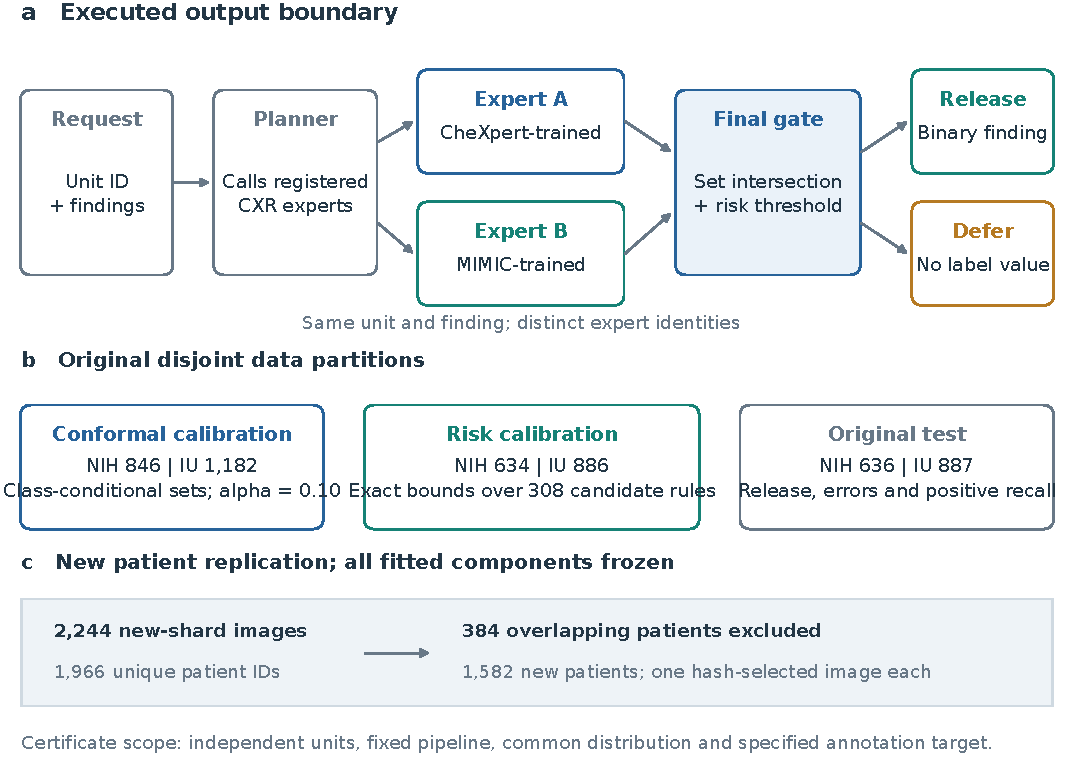
\includegraphics[width=\linewidth]{figures/fig1_architecture.pdf}
\caption{CC-Arbiter's execution path, calibration partitions and new-patient replication. The final gate returns structured binary findings or deferrals. A planner may schedule registered tools, but its free-text response is not the released finding. Both experts must concern the same unit and finding. All original NIH patients, including calibration patients, were excluded from the replication. Fitted models and gates remained frozen.}\label{fig:arch}
\end{figure}

\subsection{Independent calibration of conditional error}
For a fixed finding and threshold $t$, let $A_j(x;t)$ indicate that the proposal is eligible and $u_j(x)\leq t$. The target quantity is
\begin{equation}
R_j(t)=\Pr\{\widehat Y_j\ne\widetilde Y_j\mid A_j(X;t)=1\},
\label{eq:risk}
\end{equation}
when the conditioning event has positive probability. This is distinct from $\Pr\{\widehat Y_j\ne\widetilde Y_j, A_j=1\}$, which can be small solely because release is rare.

The threshold grid $T=\{0,0.05,\ldots,0.50\}$ was fixed before evaluation. For each proposal policy, label and threshold, the independent risk-calibration split yields $N_j(t)$ accepted units and $E_j(t)$ annotation errors. We used the exact one-sided Clopper--Pearson upper bound~\cite{cpinterval}
\begin{equation}
U_j(t)=
\begin{cases}
1, & N_j(t)=0\ \text{or}\ E_j(t)=N_j(t),\\
\operatorname{Beta}^{-1}\!\left(1-\delta/M; E_j(t)+1,N_j(t)-E_j(t)\right), & \text{otherwise},
\end{cases}
\label{eq:bound}
\end{equation}
where $\delta=0.05$ and $M=2\times2\times7\times11=308$ covers the two datasets, two calibrated policies, seven findings and eleven thresholds. For target $r$, the selected threshold is the largest $t$ with $N_j(t)>0$ and $U_j(t)\leq r$. If none qualifies, the finding always defers; zero is not used as a fallback threshold. We evaluated $r\in\{0.05,0.10,0.20\}$ with 0.10 primary. The same simultaneous bounds support all three target choices, so these targets do not create additional threshold families.

Conditional on the independently fitted conformal layer, suppose the risk-calibration and future units are identically distributed and independent. For each fixed candidate rule, the error count conditional on $N_j(t)$ is binomial with parameter $R_j(t)$. The exact upper interval is valid at tail probability $\delta/M$. A union bound gives simultaneous validity for every candidate in the family with probability at least $1-\delta$, allowing selection using the calibration data. Every selected rule then satisfies $R_j(\widehat t_j)\leq r$ on that event. Correlation across labels or experts does not invalidate the union bound; labels are never counted as additional independent binomial trials. The proof is detailed in Additional file~1. Neither monotonic conditional risk nor independence between experts is assumed. The claim is a population bound with calibration confidence, not a per-patient guarantee or a bound on the realized error of every finite test set. For IU, it additionally depends on the unverified independence of reports.

\subsection{Enforced graph execution}
The implemented graph has planning, tool-execution and final-gate nodes (Fig.~\ref{fig:arch}). Methods are registered from the initialized gated class before compilation, avoiding post-compilation class replacement. Evidence is held in invocation state and keyed by request, image or study, finding, and expert identity. Repeated calls overwrite the same expert's evidence; they never count as an additional independent expert. Mismatched image keys, failed calls, nonfinite scores, unsupported tools or missing required findings cannot supply accepted evidence. A failed repeated call invalidates its previous value.

Only the final-gate node creates the returned finding object. Released entries contain binary values; deferred entries contain no finding value and a reason or routing recommendation. A recommendation to obtain another expert or seek review is not evidence that a clinical second pass or human review occurred. We do not certify planner prose, visual question answering, segmentation masks or diagnoses synthesized beyond the seven classifier targets. Thirty-one automated tests, added in three groups as the study was extended, examine statistical edge cases and actual graph behavior, including stale evidence, cross-image mixing, repeated experts, tool failures and attempted planner overrides. The full suite is described in Additional file~1.

We additionally replayed every test unit through the actual LangGraph implementation under two deterministic schedulers: both experts in one round, and one expert per round. Tools returned the newly inferred cached scores without access to reference labels. After the tool calls, each scheduler emitted a deliberate instruction to release every finding as positive. This tested the output boundary rather than language-model reasoning. The designated final object was compared with every offline decision. These replays are software integration evaluations, not end-task LLM accuracy trials or evidence of transfer across agent frameworks.

\subsection{Comparators, outcomes and stress evaluation}
Eight prespecified policies were evaluated on identical test units: always negative; each individual expert at 0.5; mean score at 0.5; agreement of both thresholded experts; conformal singleton intersection without the risk gate; the mean-score risk gate; and CC-Arbiter. With two experts, disagreement is a tie, so the agreement baseline defers rather than fabricating a third vote. The always-negative rule illustrates the effect of class imbalance and was not itself risk-calibrated.

We report release fraction, errors divided by released opportunities, erroneous releases divided by all opportunities, and correctly released positive annotations divided by all positive annotations. The last outcome is positive recall after deferral, so rejected positives count as not recovered. Conditional error is undefined when no predictions are released. Counts are presented by finding, with pooled summaries treated as descriptive. Confidence intervals for pooled quantities use 2,000 bootstrap resamples of independent units, retaining all seven labels together, with seed 718. They condition on the fitted policy; they do not include calibration-set variability. Paired differences use the same resampled units. We make no equivalence or noninferiority claim and did not select thresholds from these intervals.

To test failure mechanisms, a uniform random number was assigned to every test unit with seed 1309. At requested corruption rates of 10\%, 25\% and 50\%, the entire seven-score vector was transformed to $1-p$ for expert B alone, or for both experts with the same mask. The same masks were used across policies, and no case was selected by correctness or reference label. Calibration remained fixed. These experiments model synthetic tool-output failures; the clean-data certificate does not cover the resulting changed score distribution.

\subsection{Secondary comparisons and newly acquired patient replication}
After inspecting the original test results, we fixed a separate, hashed enhancement protocol before acquiring additional NIH data. Analyses on the original test sets are therefore secondary and exploratory. We added two mean-score thresholds per finding: one maximizing Youden's sensitivity plus specificity minus one, and one minimizing empirical classification error. Both used only the original conformal-calibration units, with exact score candidates and ties resolved toward the largest threshold. Neither used risk-calibration or test labels. These baselines have no conditional-risk certificate and do not alter the original family of 308 candidates.

To assess the contribution of rejection, we also matched CC-Arbiter's 10\% policy release count separately for each finding. The alternatives ranked units by distance of their mean score from 0.5 or from the calibration-only Youden threshold, using the corresponding binary prediction. Ties used a hash of unit ID. The resulting batch masks use no reference labels. They are retrospective, cohort-dependent comparisons, not certified deployment policies. Paired bootstrap intervals condition on the fitted thresholds and selected masks. Finding-specific AUROC and average precision (AP), with pointwise 95\% intervals from 2,000 unit bootstrap samples, describe discrimination separately from operating-point performance. Additional file~1 specifies undefined resamples, thresholds and denominators.

We acquired the two prespecified public NIH parquet test shards, numbered 0 and 1, from the \texttt{BahaaEldin0/NIH-Chest-Xray-14} mirror, recording an immutable conversion commit and file hashes. Their 2,244 image records represented 1,966 patients. Excluding all 384 patients shared with the original NIH cohort removed 502 records. Hash-based selection of one image per remaining patient removed 160 additional views, leaving 1,582 patients with no overlap of patient IDs or selected image hashes. Both frozen experts, preprocessing, original NIH conformal quantiles and risk-gate states were reused without refitting. Secondary baseline thresholds also remained fixed. This is newly evaluated, patient-disjoint same-source replication; the data themselves were collected previously. It is not external-center or prospective clinical validation. Certificate transfer still requires a common sampling distribution, which patient disjointness alone cannot establish.

\subsection{Separate positive-sensitive review-routing study}
After the original and replication results were known, a further protocol was locked before acquiring four additional NIH shards. This extension changes the action and estimand: it flags a patient for review rather than releasing a positive diagnosis. Let $Z=1$ denote at least one of the seven annotations, and $F_t=1$ denote a review flag. We separately constrain $\Pr(F_t=0\mid Z=1)$ and $\Pr(Z=1\mid F_t=0)$ to at most 0.10. The former limits missed annotation-positive patients; the latter limits their proportion among unflagged patients. Neither is the original finding-release risk, and an unflagged patient is not declared clinically normal.

Two scores were fixed: a primary logistic stacker of the 14 expert scores, fitted only on the original 846 NIH conformal-calibration patients, and the maximum of the seven expert-mean scores. The additional 4,484 source images represented 3,518 patients. Excluding 961 patients present in either prior NIH cohort and selecting one image per remaining patient yielded 2,557 patients. A fixed random split assigned 1,278 to routing-risk calibration and 1,279 to testing, with no patient or selected-image overlap with previous cohorts. Both one-sided exact binomial bounds use $\delta=0.05$ and a separate family of $2\times41\times2=164$ score--threshold--endpoint combinations. The largest threshold meeting both constraints is selected on calibration only; otherwise all patients are flagged. A distinct final graph node enforces the review action and never supplies a diagnosis value. Additional file~1 specifies fitting, bounds, resampling and execution checks. This is a separate same-source annotation study, not an end-to-end clinical review trial.

\subsection{Use of large language models}
OpenAI Codex was used to revise code, execute the analyses, prepare programmatically generated figures and draft text. It did not generate or adjudicate any reference label, did not determine any released finding, and formed no part of the evaluated system: the released decisions come from the deterministic gate described above. Every reported quantity can be recomputed from the frozen scores in the shared archive, and the authors reviewed and approved the final content.

\section{Results}
\subsection{Coverage and informative evidence}
NIH testing comprised 636 independent patient units and 4,452 label opportunities; IU testing comprised 887 report units and 6,209 opportunities. There were 232 and 193 positive annotation targets, respectively. Across the seven labels, the CheXpert-trained and MIMIC-trained experts had NIH pooled set coverages of 89.1\% and 90.3\%, with mean set sizes of 1.55 and 1.68. IU coverages were 90.1\% and 89.9\%, with mean sizes of 1.77 and 1.73 (Fig.~\ref{fig:coverage}). These pooled quantities do not establish simultaneous or class-wise coverage. Finding-specific denominators and positive/negative coverage are provided in Additional file~1.

Rare classes impose direct limitations on informativeness. For example, only eight IU conformal-calibration reports had a pneumothorax term. At $\alpha=0.10$, the required ninth order statistic is unavailable, so the positive-class threshold becomes infinite. This behavior preserves conservative inclusion of that annotation class, but can prevent a useful negative singleton. Broad sets are therefore an expected consequence of limited calibration support, not evidence that the tool can be safely trusted or that a distribution shift has been detected.

\begin{figure}[htbp]
\centering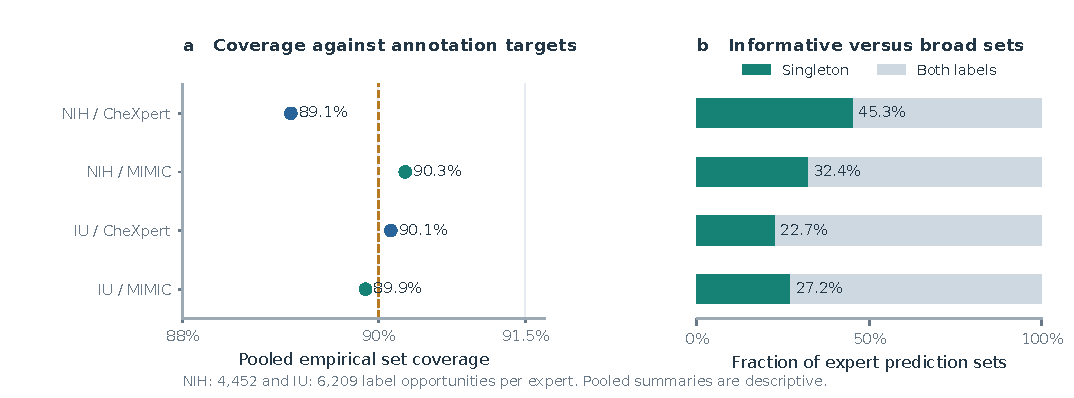
\includegraphics[width=\linewidth]{figures/fig2_coverage.pdf}
\caption{Empirical set coverage and informativeness of the two frozen experts. The dashed vertical line denotes nominal coverage for the class-conditional construction. Pooled coverage is shown descriptively; per-label class counts and coverage are in Additional file~1. There were no empty individual expert sets on these test units. A broad set contains both annotation labels.}\label{fig:coverage}
\end{figure}

\subsection{Selective error and useful release}
At the primary 10\% risk target, CC-Arbiter certified thresholds for three NIH findings: cardiomegaly, consolidation and pneumothorax. The other four findings always deferred. It released 407 of 4,452 opportunities (9.1\%; bootstrap 95\% CI, 8.1--10.2\%), with 10 annotation errors (2.5\% of releases; 95\% CI, 1.1--4.1\%). In comparison, the mean-score risk gate released 1,061 opportunities (23.8\%), with 45 errors (4.2\%). Thus, adding the conformal-intersection requirement reduced both release and erroneous release. The paired decrease in erroneous releases per all opportunities was 0.79 percentage points (95\% CI, 0.54--1.06), accompanied by a 14.69-point decrease in release (95\% CI, 13.93--15.48). This is a rejection trade-off, not evidence of superior diagnostic performance at matched release.

\begin{table}[htbp]
\centering\small\setlength{\tabcolsep}{4pt}
\caption{Primary test results at the 10\% target for the two calibrated gates. Other policies are fixed comparators without this calibration guarantee. TP denotes correctly released positive annotation targets. A dash indicates undefined conditional error.}\label{tab:main}
\input{table_results.tex}
\end{table}

On IU, none of the CC-Arbiter candidate thresholds met the required upper bound, and no finding was released. Its observed erroneous-release frequency is zero because all outputs are deferred; its conditional error is undefined. The mean-score gate released 322 of 6,209 opportunities (5.2\%), with seven errors (2.2\% of releases). Figures~\ref{fig:main} and~\ref{fig:cert} show the simultaneous calibration constraints and the resulting coverage of outputs. Increasing the target to 20\% increased NIH CC-Arbiter release to 16.3\%, but IU remained entirely deferred. At the 5\% target, NIH release was 3.1\% with no errors in 137 releases; this observation is not a zero-risk guarantee.

\begin{figure}[htbp]
\centering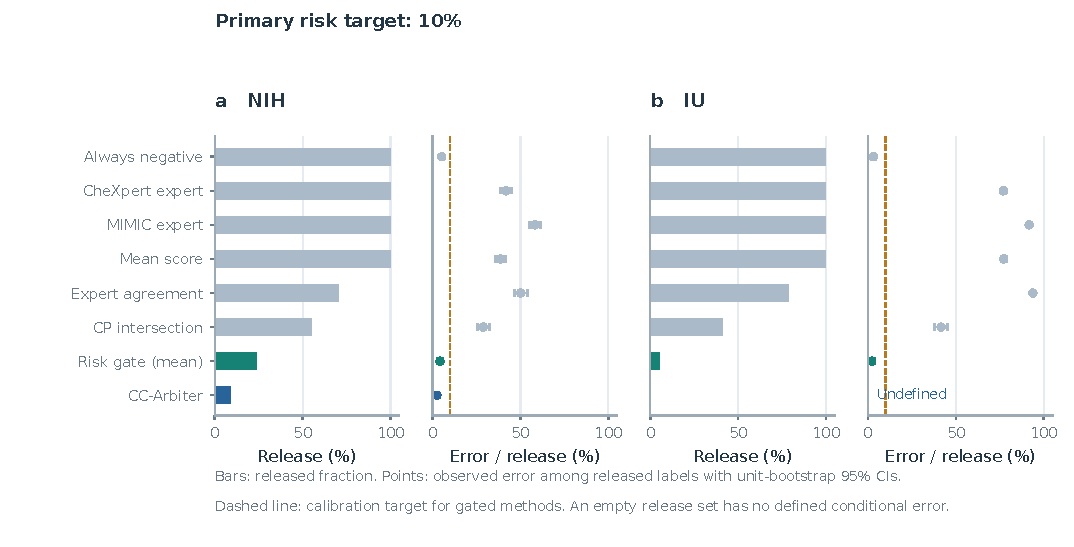
\includegraphics[width=\linewidth]{figures/fig3_selective_performance.pdf}
\caption{Release and empirical conditional error for all prespecified policies. Error intervals resample patients for NIH and reports for IU, keeping correlated labels together. A small error estimate must be interpreted with the associated release fraction and positive retention. The 10\% reference line is the calibration target of the two gated methods; it does not impose a bound on the uncalibrated comparators.}\label{fig:main}
\end{figure}

\begin{figure}[htbp]
\centering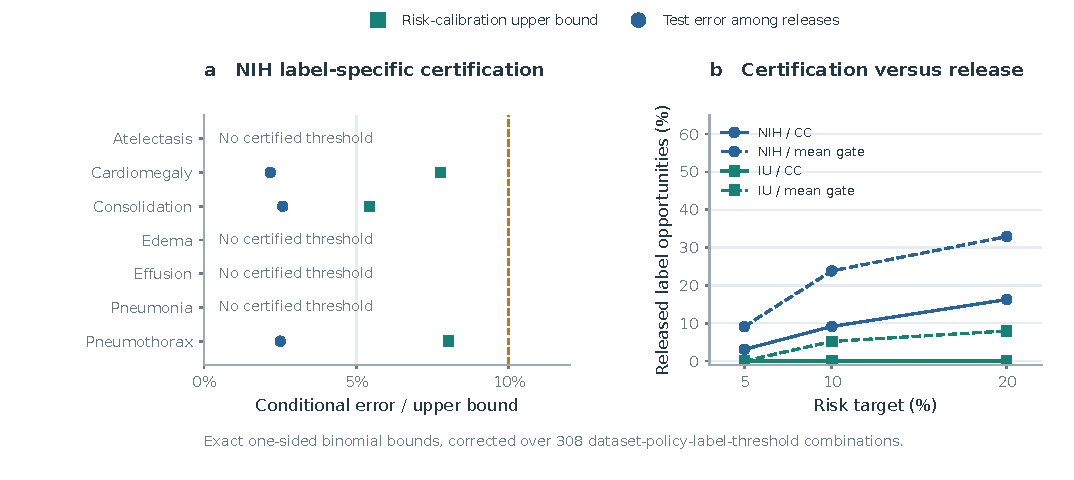
\includegraphics[width=\linewidth]{figures/fig4_risk_certificates.pdf}
\caption{Label-wise certification and its release cost. (a) NIH upper bounds on the independent risk-calibration split and observed test error for the selected CC-Arbiter thresholds. Labels without a qualifying threshold always defer. (b) Released opportunities across the three prespecified targets. Thresholds are selected using calibration only. The IU CC-Arbiter line remains at zero; no conditional-risk estimate is assigned to those empty release sets.}\label{fig:cert}
\end{figure}

The ungated experts and their mean performed poorly against these annotation targets. In particular, mean-score error was 38.7\% on NIH and 77.3\% on IU; simple agreement did not eliminate the high error (Table~\ref{tab:main}). These are properties of the specified released models, normalization, cohort subsets, view aggregation and targets. They should not be generalized to optimized classifiers or to the underlying datasets as a whole.

Class imbalance changes the interpretation of small overall error. An always-negative rule released every opportunity and had empirical error of 5.2\% on NIH and 3.1\% on IU, while recovering no positives. CC-Arbiter correctly released only 3 of 232 NIH positive targets (1.3\%); the mean-score gate recovered 4 (1.7\%). Both recovered no IU positives. Figure~\ref{fig:positive} makes this loss explicit. The observed risk reduction largely reflects withholding outputs and retaining negative annotations. It does not establish a clinically useful screening, triage or diagnostic system.

The low pooled error also did not imply a high positive predictive value. Of CC-Arbiter's eleven positive releases in the original NIH test, three matched the annotation (27.3\%); in the new patients, eight of 26 did (30.8\%). Table~\ref{tab:outcomes} gives the full decomposition of released cells together with the deferred counts. The 232 and 507 positive targets correspond to 172 and 382 patients with at least one positive annotation, so positive-label counts are not independent patient counts.

\begin{table}[htbp]
\centering\small\setlength{\tabcolsep}{5pt}
\caption{CC-Arbiter at the 10\% target, decomposed by released cell and deferral. Counts are label opportunities against the dataset annotations; PPV denotes positive predictive value. Deferred labels receive no finding value.}\label{tab:outcomes}
\input{table_outcomes.tex}
\end{table}

\begin{figure}[htbp]
\centering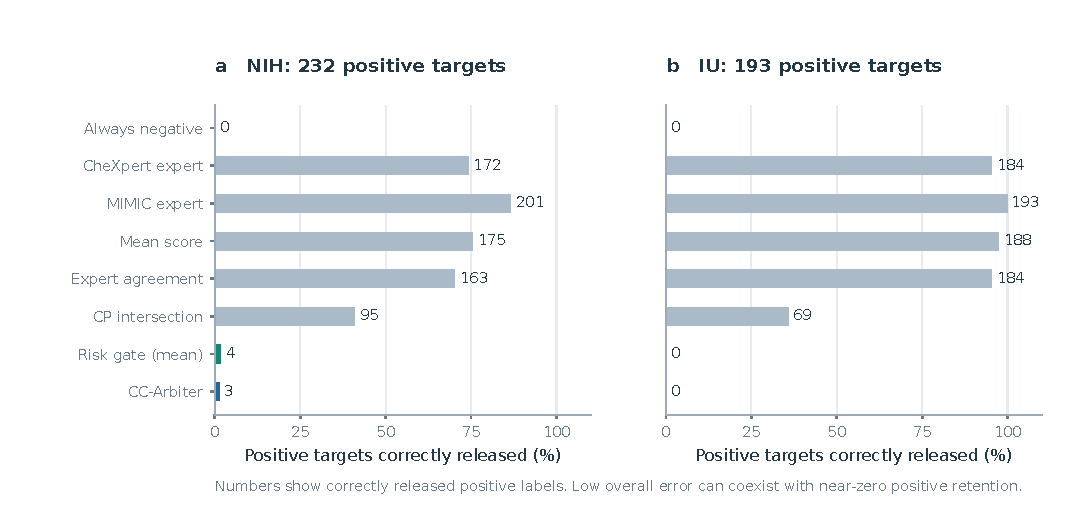
\includegraphics[width=\linewidth]{figures/fig5_positive_retention.pdf}
\caption{Positive annotation targets correctly released after deferral. Numbers next to bars give true-positive counts; the denominators are 232 NIH and 193 IU positive label opportunities. This outcome includes deferral as a failure to recover the positive target. Low pooled conditional error alone can conceal near-total loss of positive findings.}\label{fig:positive}
\end{figure}

\subsection{Correlated failures and execution fidelity}
For NIH, the requested 10\%, 25\% and 50\% masks affected 61, 145 and 325 of 636 patients. With expert B alone flipped, CC-Arbiter released 378, 328 and 238 opportunities, with 10, 10 and 6 errors, respectively. Its released error remained between 2.5\% and 3.0\%, but release decreased. These results are empirical behavior under one corruption mechanism, not an attack guarantee.

Shared corruption had a different effect. Flipping both experts for 61 patients produced 75 errors in 436 released opportunities (17.2\%). At 145 and 325 corrupted patients, error rose to 35.7\% and 62.1\%, respectively (Fig.~\ref{fig:stress}). Correlated incorrect evidence can remain mutually compatible, and clean calibration does not control its changed risk. The experiment therefore rejects a general claim of complete failure containment. IU CC-Arbiter retained its all-defer behavior because it had no certified clean threshold.

\begin{figure}[htbp]
\centering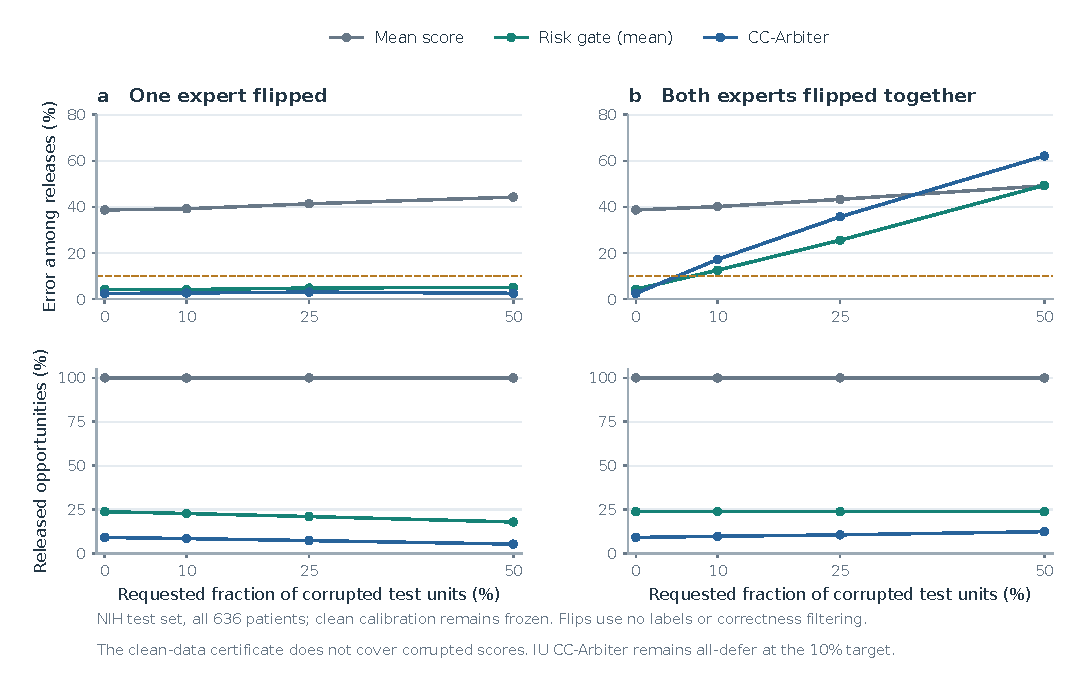
\includegraphics[width=\linewidth]{figures/fig6_correlated_failures.pdf}
\caption{NIH failure stress tests with all patients retained and identical label-independent masks across policies. The horizontal reference is the clean-data calibration target, which is not guaranteed under these corruptions. Unilateral corruption mainly reduces release, whereas shared corruption can generate confident, mutually consistent errors. The score transformation is applied at the tool-output level and does not represent a specific clinical acquisition shift.}\label{fig:stress}
\end{figure}

All 31 original and added automated tests passed. Replaying 3,105 test units, including the new NIH patients, under each of the two scheduling patterns produced 6,210 graph invocations and 43,470 final label decisions, with zero discrepancies against offline CC-Arbiter. Each invocation recorded both distinct expert outputs; deliberately conflicting planner prose did not replace the final structured decisions. Median replay time across cohorts and schedulers was approximately 1.1--2.4 ms per unit, excluding model inference and language-model calls. This verifies the implemented output boundary under the tested conditions, not negligible overhead or clinical accuracy in an end-to-end agent deployment.

\subsection{Secondary operating-point audit and patient replication}
Threshold-free discrimination was better than the poor fixed-threshold errors alone suggest (Fig.~\ref{fig:discrimination}). Mean-score AUROC ranged from 0.672 to 0.839 across findings in the original NIH test, 0.538 to 0.781 in IU, and 0.673 to 0.873 in the new NIH patients. AP and positive denominators are reported in Additional file~1; rare IU targets have especially wide uncertainty. This discrimination does not establish probability calibration or an adequate clinical operating point.

Using only conformal-calibration units to choose Youden thresholds yielded original NIH and IU mean-score errors of 41.5\% and 29.9\%, respectively, recovering 183/232 and 87/193 positive targets at full release. Thus, threshold tuning substantially improved IU performance but did not improve the NIH unweighted error. Thresholds chosen instead to minimize calibration error produced test errors of 5.2\% and 3.2\%, but recovered only two and three positive targets. These opposing outcomes illustrate the importance of defining the utility of positive findings before optimizing a threshold. They also rule out interpreting the original 0.5 baseline as the strongest possible ungated classifier.

\begin{figure}[htbp]
\centering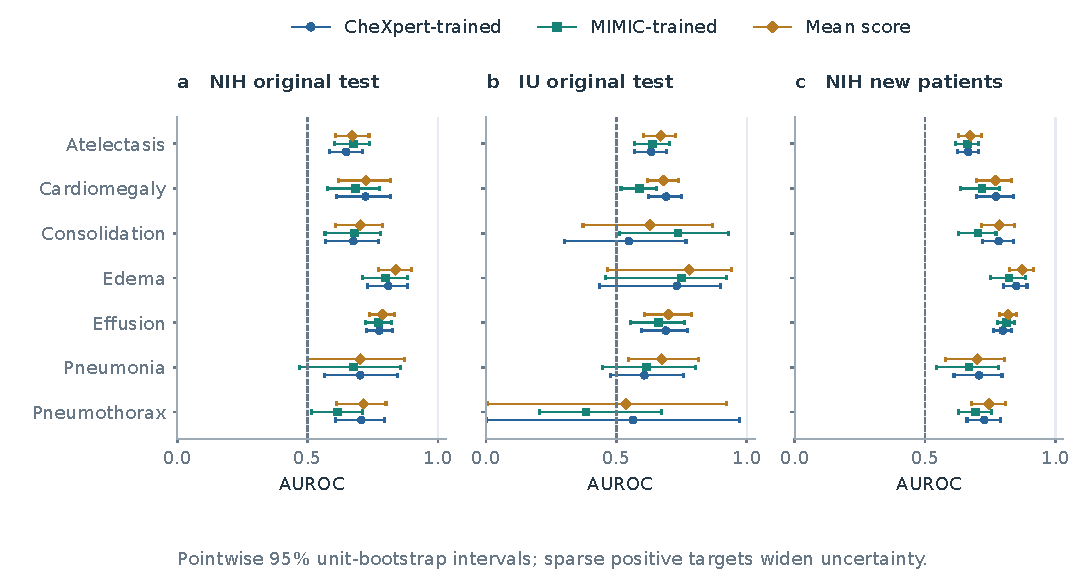
\includegraphics[width=\linewidth]{figures/fig7_discrimination.pdf}
\caption{Secondary audit of discrimination in original and new test cohorts. AUROC and pointwise 95\% intervals use unit bootstrap resampling, preserving within-unit label correlation. Intervals do not correct for comparisons across findings or models and are not used to select a policy. The vertical reference denotes AUROC 0.5. AP, positive counts and valid bootstrap counts are supplied separately.}\label{fig:discrimination}
\end{figure}

The 1,582 new NIH patients contributed 11,074 opportunities and 507 positive targets. Without recalibration, CC-Arbiter released 1,195 opportunities (10.8\%; 95\% CI, 10.1--11.5\%), with 23 errors (1.9\%; 95\% CI, 1.1--2.8\%) and eight positives recovered (1.6\% of positive targets). The mean-score risk gate released 2,949 opportunities with 91 errors and 11 recovered positives (Table~\ref{tab:replication}). The new-patient results reproduce the low-release, low-positive-retention pattern, while remaining subject to the annotation and source-sampling limitations.

\begin{table}[htbp]
\centering\small\setlength{\tabcolsep}{4pt}
\caption{Frozen-policy replication in 1,582 new NIH patients: 11,074 label opportunities and 507 positive targets. TP and recall concern correctly released positive annotations. Gates use the original 10\% target. Matched rules share CC-Arbiter's release count for every finding, use no new target labels for selection and have no risk certificate.}\label{tab:replication}
\input{table_replication.tex}
\end{table}

At identical per-label release counts, simple mean-score ranking produced five errors among 407 original NIH releases and 14 among 1,195 new-patient releases, versus CC-Arbiter's 10 and 23 errors (Fig.~\ref{fig:matched}). The CC-minus-ranking conditional-error differences were 1.23 percentage points (paired 95\% CI, 0.28--2.41) and 0.75 points (0.09--1.50), conditional on the fitted thresholds and chosen batch masks. Ranking recovered fewer positives: zero versus three originally, and three versus eight in replication. Youden-based matched ranking recovered more positives (six and 25) but incurred more errors (50 and 123). These are descriptive trade-offs, not a multiplicity-adjusted superiority trial. IU had no nonzero CC-Arbiter release budget, so a matched-release conditional-error comparison was undefined.

\begin{figure}[htbp]
\centering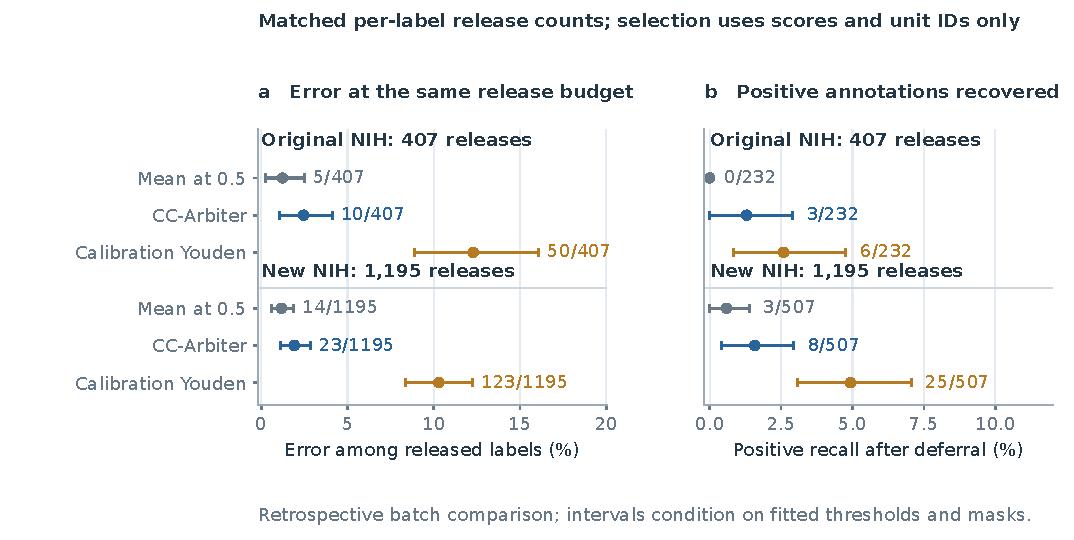
\includegraphics[width=\linewidth]{figures/fig8_matched_replication.pdf}
\caption{Error and positive recall at exactly matched per-finding release counts in two disjoint NIH test cohorts. Mean and Youden ranking select by distance from the corresponding score threshold; ties use a hash of unit ID. Points and intervals use the same patient bootstrap samples, conditional on the observed batch selections. Numerators and denominators are shown explicitly. No comparator uniformly improves both error and positive retention.}\label{fig:matched}
\end{figure}

\subsection{Post hoc projection-stratified audit}
After the primary results were known, we additionally tabulated release, error and positive recovery separately for anteroposterior (AP) and posteroanterior (PA) examinations in both NIH cohorts. Policies, thresholds, calibration states and the reference annotations were unchanged. In the original NIH test, CC-Arbiter released 42 of 1,610 AP opportunities (2.6\%) with seven errors among releases (16.7\%; pointwise patient-bootstrap 95\% CI, 6.3--29.4\%) and 365 of 2,842 PA opportunities (12.8\%) with three errors (0.8\%; 95\% CI, 0.0--1.9\%). The new-patient cohort showed the same ordering: 122 of 3,717 AP opportunities (3.3\%; 5.7\% error; 95\% CI, 1.8--10.1\%) and 1,073 of 7,357 PA opportunities (14.6\%; 1.5\%; 95\% CI, 0.7--2.4\%) (Table~\ref{tab:subgroups}). These analyses were not prespecified and were not adjusted for differences in patient or released-label composition; they carry no projection-specific risk guarantee, and the AP intervals are wide because few labels were released there.

\begin{table}[htbp]
\centering\footnotesize\setlength{\tabcolsep}{3.5pt}
\caption{Post hoc projection-stratified audit in both NIH cohorts with all policies frozen. Intervals are pointwise patient-bootstrap percentile intervals within each stratum and are not multiplicity-adjusted or calibrated as subgroup guarantees.}\label{tab:subgroups}
\input{table_subgroups.tex}
\end{table}

\subsection{Certification feasibility}
For a candidate with zero observed errors, the exact upper bound is $1-(\delta/M)^{1/n}$. Therefore, at least 171, 83 and 40 accepted risk-calibration units are necessary to certify targets of 5\%, 10\% and 20\%, respectively; any observed errors raise the requirement. These are accepted counts for one fixed candidate, not total cohort sizes or counts pooled across findings. For IU at 10\%, each finding had at least one candidate with 83 or more accepted units, yet no candidate met the error bound. Sample scarcity alone therefore does not explain its all-defer result. Minimum candidate upper bounds ranged from 0.318 to 1.000, compared with 0.046 to 0.239 for NIH. Full counts and bounds are in Additional file~1.

\subsection{Positive attrition and review-routing feasibility}
The original NIH mean-score rule correctly released 175 of 232 positive annotations, the conformal intersection 95, and CC-Arbiter only three (Fig.~\ref{fig:review}a). Moreover, only three of CC-Arbiter's eleven positive releases matched the positive annotation, illustrating that its low pooled error does not imply high positive predictive value. In IU the corresponding correct-positive counts were 188, 69 and zero. The intersection and the risk gate both contribute to positive loss; these summaries do not imply that the intermediate positive sets are nested.

The separate routing-calibration set contained 250 annotation-positive patients. Neither score had a threshold satisfying both 10\% upper bounds (Fig.~\ref{fig:review}b). The minimum upper bound on positivity among unflagged patients was 12.7\% for stacking and 11.6\% for maximum mean, already exceeding the target. Consequently, both selected policies flagged all 1,279 test patients, including all 267 annotation-positive patients. This is the structural all-flag fallback, not an improvement in automatic positive diagnosis, and it reduces no review flags. Fixed 0.5 comparators illustrate the opposing error: the stacker flagged only 73/267 positive patients and maximum mean 216/267, without the specified certificates. Their full counts are in Additional file~1. No actual human reviews or clinical workload savings were measured.

\begin{figure}[htbp]
\centering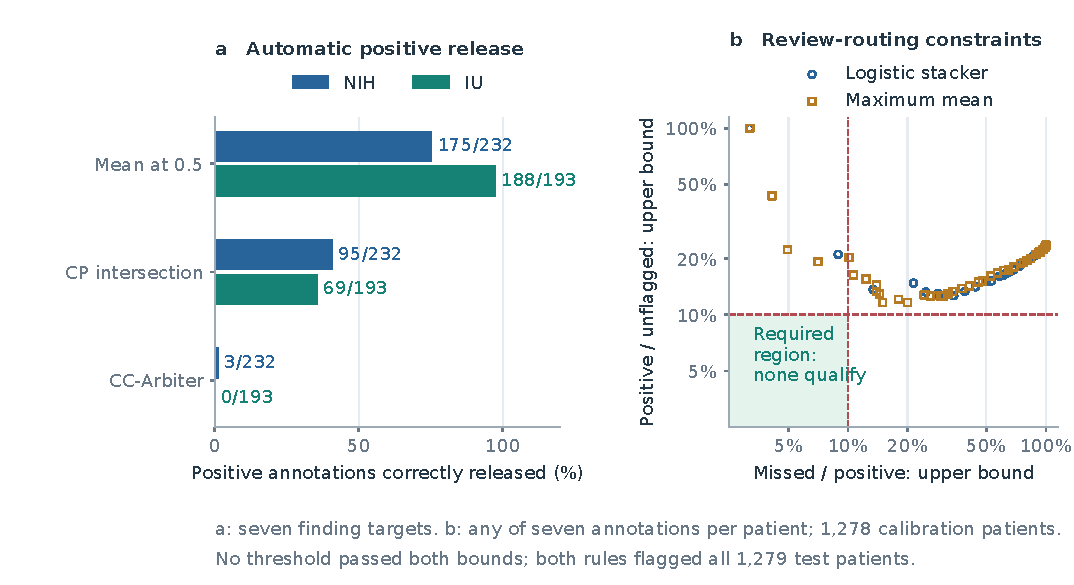
\includegraphics[width=\linewidth]{figures/fig9_positive_review.pdf}
\caption{Positive loss and the feasibility of a separate review action. (a) Correctly released positive annotations in the original tests; the methods are not assumed to form nested positive subsets. (b) Simultaneous exact calibration bounds for 41 thresholds under each of two routing scores. The shaded region requires both bounds at most 10\%; no candidate falls inside it. Axes in panel b are logarithmic. The calibration unit and target differ from panel a: patients with any of seven annotations. All-flag routing does not constitute automatic diagnosis or measured workload reduction.}\label{fig:review}
\end{figure}

\section{Discussion}
This study separates three often conflated properties: calibrated set inclusion, conditional-risk selection, and software enforcement. Individual conformal sets can have coverage close to nominal while their singleton intersection has high selective error. A separately calibrated gate can limit that error while retaining very little evidence. A final graph node can enforce the resulting rule even when the planner proposes a different answer. None of these properties establishes the clinical value of the released findings.

The comparisons with simpler selection are central. Both calibrated gates use the same independent calibration split, candidate thresholds and family correction; the mean-score gate released more labels. At identical per-label budgets, mean-score ranking incurred fewer errors than CC-Arbiter in both NIH cohorts, although it also recovered fewer positives. The conformal-intersection stage is therefore not established as necessary or more efficient. Its role here is to make evidence compatibility explicit. The separately locked new-patient replication strengthens the evidence for this trade-off without converting the secondary original-test analyses into prespecified primary findings.

The all-negative comparator further limits interpretation. With positive annotation rates of only 5.2\% and 3.1\%, unweighted error is an incomplete clinical objective. Our exact bounds control that defined error, but they do not constrain sensitivity, false-negative risk within positive cases, or the clinical cost of missed disease. A system that refuses nearly every positive output cannot be justified by a small pooled error alone. Useful extensions would prespecify class-sensitive losses or simultaneous sensitivity and predictive-value requirements, using enough independently labelled positive cases to calibrate them. Optimizing such requirements after viewing these test results would require a new validation set.

Correlated failure is another boundary. Experts trained on different sources still share an architecture and can fail together. Intersected sets check compatibility rather than truth; they can agree on an incorrect label. We did not assume expert independence in the proof, but the proof does require calibration and future units to follow the same pipeline and distribution. Our corruption changes that distribution. The observed increase to 17.2\% error after joint flips in 9.6\% of NIH patients is therefore consistent with the guarantee's stated domain and shows why it must not be presented as adversarial robustness.

Several limitations affect external validity. The NIH analyses used two original shards, two additional shards for the frozen-policy replication and four further shards for the separate review-routing study, with one hash-selected image per patient throughout. All three patient cohorts were disjoint in the available identifiers and selected-image hashes. They came from the same source, so they do not provide external-centre validation. IU images form a locally available subset, and report-level aggregation includes lateral views. Stable cross-report patient identifiers are unavailable. The secondary threshold audit changes operating points but neither retrains experts nor calibrates their scores as disease probabilities. Label rarity can make conformal thresholds infinite and exact risk bounds conservative, while observed errors can independently prevent certification even when accepted counts are adequate. The study uses text-mined or report-indexing targets without new radiologist adjudication. An error against those targets need not be a clinical error, and agreement need not be clinical correctness. Bootstrap intervals condition on fitted calibration layers and do not capture their sampling variability. Results concern the specified processing and annotation task rather than diagnostic deployment.

Our bounds were calibrated by finding within each data source and were not conditioned on projection, age or the recorded sex field. The post hoc AP/PA differences therefore describe where released outputs occurred rather than a calibrated subgroup guarantee, and they may reflect differences in patient and released-label composition as well as projection-related model behaviour.

The Bonferroni-corrected exact procedure is deliberately simple and can be statistically inefficient. The additional routing study also failed to certify a reduction in review flags under the specified dual objective. It does not prove that all routing scores or calibration methods must fail; it shows that these fixed experts, scores, sample sizes and constraints did not suffice. We did not compare the release efficiency of newer selective-risk methods such as SCoRE~\cite{score}; no optimality claim is made. Deterministic graph replay does not evaluate natural language planning, clinical second-pass resolution or actual human review. Better image-model discrimination, clinically adjudicated targets and independently validated utilities remain necessary before claiming useful clinical performance.

\begin{samepage}
\section{Conclusions}
CC-Arbiter makes finite-sample risk calibration and selective output enforcement jointly auditable. Original and replication NIH cohorts showed low conditional error accompanied by extensive rejection and poor positive retention; IU yielded no certified release. Mean-score ranking had fewer errors at matched release counts but retained fewer positives. A separate positive-sensitive routing study also failed to certify a reduction in review flags, while shared expert corruption defeated clean-data control. The findings support reporting assumptions, execution, release, positive retention and action-specific utility together; they establish neither clinical deployment readiness nor a general accuracy advantage.
\end{samepage}

\section*{Abbreviations}
AP: anteroposterior projection (the ranking metric average precision is written in full); AUROC: area under the receiver operating characteristic curve; CI: confidence interval; FN: false negative; FP: false positive; IU: Indiana University chest radiograph collection; LLM: large language model; MeSH: Medical Subject Headings; NIH: National Institutes of Health ChestX-ray14 collection; PA: posteroanterior projection; PPV: positive predictive value; TF32: TensorFloat-32; TN: true negative; TP: true positive.

\section*{Declarations}
\paragraph{Ethics approval and consent to participate.} This work is a secondary computational analysis of two publicly available, de-identified chest radiograph datasets, NIH ChestX-ray14 and the Indiana University collection. No participants were recruited or contacted, no new clinical data were collected, no intervention was performed and no identifiable information is reported. Because the study uses only previously collected, publicly released, de-identified data, ethics approval and participant consent were not required, and no ethics committee reference number applies. Consent and data-use terms for the original collections were administered by the dataset providers. The authors confirmed this determination with the supervising faculty member (X.~Kong, 12 October 2026).
\paragraph{Consent for publication.} Not applicable. No identifiable individual information or participant images are reproduced in this manuscript.
\paragraph{Availability of data and materials.} The datasets analysed are publicly available and fully cited in the reference list: the NIH ChestX-ray14 collection~\cite{nih} and the Indiana University chest radiograph collection~\cite{iu}. Derived files supporting the conclusions, including the frozen split manifests, expert scores, calibrated thresholds, per-unit decisions and machine-readable results, are included within the article's additional files. Project name: CC-Arbiter reproducibility archive. Project home page: https://github.com/binghe-glacier/cc-arbiter; the same archive accompanies this submission as Additional file~2. Archived version: Zenodo, https://doi.org/10.5281/zenodo.23329663. Operating system: platform independent, developed and tested on Windows~11. Programming language: Python (3.11). Other requirements: NumPy, SciPy and Matplotlib for analysis from the supplied scores; LangGraph and LangChain Core for execution replay; PyTorch and TorchXRayVision for optional re-inference, which additionally requires network access to download public model weights. License: MIT. Restrictions for non-academics: none stated beyond the terms of the source datasets. Original radiographs, report text and pretrained weights are not redistributed and remain subject to their providers' terms.
\paragraph{Competing interests.} The authors declare that they have no competing interests.
\paragraph{Funding.} This research received no specific grant from any funding agency in the public, commercial, or not-for-profit sectors.
\paragraph{Authors' contributions.} YY: Conceptualization, Methodology, Software, Formal analysis, Investigation, Data curation, Visualization, Writing (original draft). XK: Supervision, corresponding author.
\paragraph{Acknowledgements.} Not applicable.

\paragraph{Generative AI assistance.} OpenAI Codex assisted with code revision, execution of the analyses, preparation of programmatically generated figures and manuscript drafting. It produced no reference labels and no released findings. The authors are responsible for verifying and approving the final submitted content.
\paragraph{Additional files.} Additional file~1: supplementary methods, statistical proof, cohort composition, post hoc subgroup descriptives, cohort-level positive counts and detailed calibration results (PDF). Additional file~2: reproducibility archive containing executable code, fixed derived scores, split manifests, machine-readable results and provenance records (ZIP). Original images, report text and model weights are excluded from both files.
\begin{thebibliography}{99}
\small
\bibitem{medrax} Fallahpour A, Ma J, Munim A, Lyu H, Wang B. MedRAX: Medical reasoning agent for chest X-ray. 2025. arXiv:2502.02673.
\bibitem{cxragent} Lou J, Yang Y, Yu Z, Fu Z, Han W, Huang Q, Yu J. CXRAgent: Director-orchestrated multi-stage reasoning for chest X-ray interpretation. 2025. arXiv:2510.21324.
\bibitem{radagents} Zhang K, Barrett CD, Kim J, Sun L, Taghavi T, Kenthapadi K. RadAgents: Multimodal agentic reasoning for chest X-ray interpretation with radiologist-like workflows. MIDL 2026. arXiv:2509.20490.
\bibitem{vovk} Vovk V, Gammerman A, Shafer G. Algorithmic learning in a random world. Springer; 2005.
\bibitem{gentle} Angelopoulos AN, Bates S. A gentle introduction to conformal prediction and distribution-free uncertainty quantification. 2021. arXiv:2107.07511.
\bibitem{ltt} Angelopoulos AN, Bates S, Cand\`es EJ, Jordan MI, Lei L. Learn then test: Calibrating predictive algorithms to achieve risk control. 2021. arXiv:2110.01052.
\bibitem{crc} Angelopoulos AN, Bates S, Fisch A, Lei L, Schuster T. Conformal risk control. ICLR 2024. arXiv:2208.02814.
\bibitem{score} Bai T, Jin Y. Conformal selective prediction with general risk control. 2026. arXiv:2603.24704.
\bibitem{coma} Gasparin M, Ramdas A. Conformal online model aggregation. arXiv:2403.15527. Revised 2025.
\bibitem{nih} Wang X, Peng Y, Lu L, Lu Z, Bagheri M, Summers RM. ChestX-ray8: Hospital-scale chest X-ray database and benchmarks on weakly-supervised classification and localization of common thorax diseases. Proceedings of CVPR. 2017. arXiv:1705.02315.
\bibitem{iu} Demner-Fushman D, Kohli MD, Rosenman MB, et al. Preparing a collection of radiology examinations for distribution and retrieval. J Am Med Inform Assoc. 2016;23:304--310. doi:10.1093/jamia/ocv080.
\bibitem{xrv} Cohen JP, Viviano JD, Bertin P, et al. TorchXRayVision: A library of chest X-ray datasets and models. 2021. arXiv:2111.00595.
\bibitem{densenet} Huang G, Liu Z, van der Maaten L, Weinberger KQ. Densely connected convolutional networks. Proceedings of CVPR. 2017. arXiv:1608.06993.
\bibitem{chex} Irvin J, Rajpurkar P, Ko M, et al. CheXpert: A large chest radiograph dataset with uncertainty labels and expert comparison. 2019. arXiv:1901.07031.
\bibitem{mimic} Johnson AEW, Pollard TJ, Berkowitz SJ, et al. MIMIC-CXR, a de-identified publicly available database of chest radiographs with free-text reports. Sci Data. 2019;6:317. doi:10.1038/s41597-019-0322-0.
\bibitem{cpinterval} Clopper CJ, Pearson ES. The use of confidence or fiducial limits illustrated in the case of the binomial. Biometrika. 1934;26:404--413. doi:10.1093/biomet/26.4.404.
\end{thebibliography}
\end{document}
;
% the compact reading version omits it.
\usepackage{setspace}
\renewcommand{\rmdefault}{ptm}
\renewcommand{\sfdefault}{phv}
\renewcommand{\ttdefault}{phv}
% Font setup that compiles under both engines.
% XeTeX/Tectonic: native OpenType Times/Arial declarations, no extra packages.
% pdfLaTeX (used by the journal's TeX Live 2021 build): standard PS fonts.
\ifdefined\XeTeXversion
\DeclareFontFamily{TU}{ccserif}{}
\DeclareFontShape{TU}{ccserif}{m}{n}{<->"[local-fonts/times.ttf]"}{}
\DeclareFontShape{TU}{ccserif}{m}{it}{<->"[local-fonts/timesi.ttf]"}{}
\DeclareFontShape{TU}{ccserif}{b}{n}{<->"[local-fonts/timesbd.ttf]"}{}
\DeclareFontShape{TU}{ccserif}{bx}{n}{<->"[local-fonts/timesbd.ttf]"}{}
\DeclareFontShape{TU}{ccserif}{b}{it}{<->"[local-fonts/timesbi.ttf]"}{}
\DeclareFontShape{TU}{ccserif}{bx}{it}{<->"[local-fonts/timesbi.ttf]"}{}
\DeclareFontFamily{TU}{ccsans}{}
\DeclareFontShape{TU}{ccsans}{m}{n}{<->"[local-fonts/arial.ttf]"}{}
\DeclareFontShape{TU}{ccsans}{b}{n}{<->"[local-fonts/arialbd.ttf]"}{}
\DeclareFontShape{TU}{ccsans}{bx}{n}{<->"[local-fonts/arialbd.ttf]"}{}
\DeclareFontShape{TU}{ccsans}{m}{it}{<->"[local-fonts/ariali.ttf]"}{}
\renewcommand{\rmdefault}{ccserif}
\renewcommand{\sfdefault}{ccsans}
\renewcommand{\ttdefault}{ccsans}
\else
\usepackage[T1]{fontenc}
\usepackage{mathptmx}
\usepackage[scaled=0.92]{helvet}
\renewcommand{\ttdefault}{phv}
\fi

\DeclareMathSizes{12}{10}{7}{5}
\DeclareMathSizes{9}{10}{7}{5}
\makeatletter\renewcommand\normalsize{\@setfontsize\normalsize{12}{15}}\makeatother
\normalsize
\setlength{\textwidth}{166mm}
\setlength{\textheight}{242mm}
\setlength{\oddsidemargin}{-3mm}
\setlength{\evensidemargin}{-3mm}
\setlength{\topmargin}{-15mm}
\setlength{\parskip}{3pt}
\setlength{\parindent}{12pt}
\setlength{\emergencystretch}{2em}
\renewcommand{\baselinestretch}{1.09}
\ifdefined\REVIEWCOPY\usepackage{lineno}\AtBeginDocument{\doublespacing\linenumbers}\fi
\renewcommand{\topfraction}{0.92}\renewcommand{\bottomfraction}{0.85}
\renewcommand{\textfraction}{0.06}\renewcommand{\floatpagefraction}{0.78}
\title{Auditing selective release of chest radiograph findings: retrospective evaluation of CC-Arbiter}
\author{Yaocong Yang and Xiangyong Kong\\[4pt]
\small School of Health Science and Engineering,\\
\small University of Shanghai for Science and Technology, Shanghai, China\\
\small Correspondence: Xiangyong Kong, \texttt{kxy@usst.edu.cn}}
\date{}
\begin{document}
\maketitle
\begin{abstract}
\noindent\textbf{Background:} Low error among selectively released chest radiograph findings can conceal the rejection of nearly all positive findings. We evaluated an executable evidence gate and audited its release, positive retention and failure boundaries.\par
\noindent\textbf{Methods:} CC-Arbiter intersects class-conditional conformal sets from two frozen DenseNet-121 experts and applies independently calibrated conditional-error gates using exact, multiplicity-corrected binomial bounds. The original cohorts comprised 2,116 NIH patients and 2,955 IU reports, with disjoint conformal, risk-calibration and test splits. Seven dataset annotations served as targets, without new clinical adjudication. A secondary protocol added calibration-only threshold baselines, score discrimination and comparisons at matched release counts. Frozen policies were then evaluated in 1,582 additional NIH patients absent from the original cohort. A separate review-routing study used 2,557 additional NIH patients, split into independent risk-calibration and test sets. It constrained both missed positives and positivity among unflagged patients. Projection-stratified results were examined post hoc. Score corruption and graph execution were also assessed.\par
\noindent\textbf{Results:} At the 10\% risk target, CC-Arbiter released 407/4,452 original NIH opportunities (9.1\%), with 10 errors (2.5\%; unit-bootstrap 95\% confidence interval, 1.1--4.1\%) and only 3/232 positive targets recovered. Positive predictive value was 27.3\%. It released nothing on IU. New-patient replication yielded 1,195/11,074 releases (10.8\%), 23 errors (1.9\%; 95\% confidence interval, 1.1--2.8\%), 8/507 positive targets recovered and positive predictive value of 30.8\%. Anteroposterior examinations received fewer and more erroneous releases than posteroanterior ones (originally 2.6\% versus 12.8\% release; 16.7\% versus 0.8\% error). Simple mean-score ranking at identical per-label release counts produced fewer errors in both NIH cohorts (5 and 14), while recovering fewer positives (0 and 3). Calibration-only Youden thresholds reduced IU mean-score error from 77.3\% to 29.9\%. Shared corruption in 61/636 original NIH patients raised CC-Arbiter error to 17.2\%. Both routing procedures flagged all 1,279 new test patients because no threshold met both constraints. All 43,470 original and replication label decisions matched offline gating.\par
\noindent\textbf{Conclusions:} The framework makes risk calibration and output enforcement auditable, but low selective error did not establish useful positive retention or superiority over simpler selection. Replication supports joint reporting of release, positive recall, matched-budget comparisons and correlated failures.
\end{abstract}
\noindent\textbf{Keywords:} chest radiograph; selective prediction; conformal prediction; risk control; medical imaging agents; reproducibility

\section{Background}
Medical imaging agents combine a planning model with specialist tools for image classification, visual question answering, segmentation and report generation. MedRAX introduced a unified chest radiograph tool interface and the ChestAgentBench benchmark~\cite{medrax}. CXRAgent and RadAgents further develop staged verification and radiologist-inspired workflows~\cite{cxragent,radagents}. These systems motivate a practical engineering question: which tool-derived statements may reach the user when experts disagree or provide uncertain evidence? Providing confidence information to a language model and enforcing an output rule are different operations. A model may disregard an uncertainty annotation, and a correctly written monitor may still be absent from the executed graph.

Conformal prediction provides one component of a solution. Given suitable calibration data and exchangeability, it constructs prediction sets with finite-sample coverage~\cite{vovk,gentle}. Coverage concerns whether a set contains the specified target; it does not by itself bound error among the subset of outputs that a system chooses to release. Intersecting multiple sets, selecting a singleton and withholding some predictions introduce further selection. A separate selective-risk argument is therefore needed. Moreover, a guarantee against imperfect dataset annotations does not become a guarantee against clinical diagnoses.

Risk calibration methods address several different objectives. Learn Then Test calibrates predictive procedures through hypothesis testing~\cite{ltt}. Conformal Risk Control addresses expected bounded losses under its assumptions~\cite{crc}; a joint wrong-and-released loss is not the conditional error among released predictions. SCoRE studies selective risk more directly~\cite{score}. Work on conformal model aggregation also shows that combining prediction sets requires its own analysis~\cite{coma}. Our aim is not to introduce a new conformal theorem. We implement a transparent finite-family procedure whose statistical unit, release rule and software execution can all be checked.

The resulting system, CC-Arbiter, operates on two classifier outputs for the same image or study and finding. It constructs a proposal from intersected conformal sets, calibrates whether that proposal can be released, and replaces the planner's final prose with a structured release-or-defer decision. We evaluate three questions: whether the final gate executes as specified; how much evidence remains after conditional-risk calibration; and whether low overall error is accompanied by useful positive findings or robustness to shared expert failures. The contribution is an auditable implementation and empirical assessment of these questions, including cases where the gate cannot certify useful output.

\section{Methods}
\subsection{Study design and annotation targets}
This retrospective computational study used NIH ChestX-ray14 and IU chest radiograph data~\cite{nih,iu}. The original analysis specification, threshold grid and split manifest were fixed before revised image-model inference and evaluation. This was an internal analysis lock, not public preregistration or a prospectively collected clinical cohort. The pretrained image experts were not fitted on either evaluation dataset. A later, separately specified review-routing extension fits a small score-combination model on original calibration patients only. The primary estimand is error with respect to seven specified dataset annotations: atelectasis, cardiomegaly, consolidation, edema, effusion, pneumonia and pneumothorax.

For NIH, both complete local parquet shards contained 2,458 image records from 2,116 patients. One image per patient was selected using the lexicographically smallest SHA-256 digest of its encoded image bytes, independently of labels and predictions. The resulting 2,116 units contain no duplicated selected image across patient identifiers. We used the released text-mined finding labels, restricted to the seven supported categories. These labels are not newly obtained expert adjudications. The cohort is an available subset of NIH, not the full dataset or an official challenge test set.

For IU, 3,955 XML reports were available; 2,955 had locally available linked PNG images. All linked reports were retained regardless of whether a selected finding was present, including normal reports. Three duplicate image copies within reports were removed, leaving 6,088 distinct report-linked images. Each target is the presence of its prespecified MeSH term in the report's major or minor terms, using the trunk before any slash. For example, \emph{Pleural Effusion} maps to effusion. Absence of a mapped term defines annotation target zero; it is not evidence that the finding is clinically absent. The exact mapping is in Additional file~1. Expert scores were aggregated by their maximum over all available views of a report. This fixed study-level rule includes lateral views and can impair specificity; we did not use outcomes to select a view or aggregation rule. Report identifiers were available, but stable patient identifiers across IU reports were not. Accordingly, patient independence can be enforced for NIH but is only an assumption for IU report-level analyses.

Within each dataset, sorted unit identifiers were shuffled with NumPy's \texttt{default\_rng(20261009)}. The first $\lfloor0.4n\rfloor$ units were assigned to conformal calibration, the next $\lfloor0.3n\rfloor$ to risk calibration, and the remainder to testing (Table~\ref{tab:cohort}). There was no overlap of unit identifiers across splits. All views of an IU report remained together. No image failed the revised inference pipeline. Dataset labels were used only in the appropriate calibration steps or for final scoring, never by the prediction or corruption functions.

\begin{table}[htbp]
\centering\small
\caption{Disjoint calibration and test units. NIH contributes one selected image per patient. IU contributes all available views per report; cross-report patient independence is unverified.}\label{tab:cohort}
\begin{tabular}{llrrrr}
\toprule
Dataset & Unit & Conformal & Risk calibration & Test & Total images\\
\midrule
NIH & Patient & 846 & 634 & 636 & 2,116\\
IU & Report & 1,182 & 886 & 887 & 6,088\\
\bottomrule
\end{tabular}
\end{table}

Table~\ref{tab:characteristics} describes the analysed units, including age, the source dataset's sex field and projection. These descriptors are reported for completeness: the risk bounds were calibrated by finding within each data source and not within demographic or projection strata.

\begin{table}[htbp]
\centering\small\setlength{\tabcolsep}{3.5pt}
\caption{Composition of the analysed cohorts. Source sex is the datasets' recorded Patient Gender field and is not interpreted as biological sex or gender identity. IU report-level descriptors other than image counts and positive targets were not available.}\label{tab:characteristics}
\begin{tabular}{lrrrrrrr}
\toprule
Cohort (unit) & $n$ & Age, median [Q1, Q3] & Range & $<18$ & Source sex (M/F) & AP/PA & Positive targets\\
\midrule
NIH conformal (patient) & 846 & 49 [35, 59] & 2--86 & 47 & 473/373 & 302/544 & 287\\
NIH risk calibration & 634 & 49 [34, 59] & 9--87 & 29 & 361/273 & 220/414 & 178\\
NIH test & 636 & 49 [36, 59] & 2--94 & 23 & 345/291 & 230/406 & 232\\
NIH new replication & 1,582 & 49 [35, 59] & 2--88 & 67 & 898/684 & 531/1,051 & 507\\
NIH routing risk calibration & 1,278 & 48 [34, 58] & 2--82 & 62 & 710/568 & 363/915 & 334\\
NIH routing test & 1,279 & 49 [35, 59] & 3--93 & 61 & 675/604 & 367/912 & 339\\
IU conformal (report) & 1,182 & -- & -- & -- & -- & -- & 283\\
IU risk calibration & 886 & -- & -- & -- & -- & -- & 196\\
IU test & 887 & -- & -- & -- & -- & -- & 193\\
\bottomrule
\end{tabular}\par\vspace{3pt}
\noindent\footnotesize IU images numbered 2,435, 1,827 and 1,826 in the three splits; each NIH patient contributes one selected image. Positive targets are label opportunities and may overlap within a unit. Age quantiles use linear interpolation and are shown as integers.

\end{table}

\subsection{Frozen expert models and preprocessing}
We used TorchXRayVision~\cite{xrv} releases \texttt{densenet121-res224-chex} and \texttt{densenet121-res224-mimic\_ch}. Both use DenseNet-121~\cite{densenet}; their documented training sources are CheXpert~\cite{chex} and MIMIC-CXR~\cite{mimic}, respectively. Thus, the comparison uses different training sources, not different backbone architectures. The selected weight releases do not list NIH or IU as training sources. This source-level audit is not a record-level comparison against the original training databases. Download URLs and SHA-256 weight digests are included with the code.

Each image was decoded to grayscale, normalized to approximately $[-1024,1024]$, centrally cropped, and resized to $224\times224$ with TorchXRayVision's scikit-image resizer. Inference used fixed evaluation-mode models and float32 arithmetic on an NVIDIA RTX 4090, with TF32 disabled. TorchXRayVision's published operating-point normalization was retained. Consequently, the outputs $p_{ej}(x)\in[0,1]$ are model scores, not validated probabilities of disease. Fixed baselines threshold these scores at 0.5. Sixteen randomly selected images were independently rerun one at a time; the maximum absolute deviation from batched scores was below $10^{-6}$. The preprocessing and weight versions were identical across calibration and testing.

\subsection{Conformal evidence and proposal formation}
Let $e\in\{1,2\}$ index experts, $j\in\{1,\ldots,7\}$ index findings, and $\widetilde Y_j\in\{0,1\}$ denote the annotation target. For each expert, finding and target class $c$, the calibration score is $s_{ej}(x,c)=|c-p_{ej}(x)|$. If there are $n_{jc}$ calibration units with $\widetilde Y_j=c$, the threshold is the $\lceil(n_{jc}+1)(1-\alpha)\rceil$-th ordered score. It is $+\infty$ if the required rank exceeds $n_{jc}$, including when that class is absent. We used $\alpha=0.10$ throughout. The class-conditional set is
\begin{equation}
C_{ej}(x)=\{c\in\{0,1\}: |c-p_{ej}(x)|\leq q_{ejc}\}.
\label{eq:sets}
\end{equation}
For a fixed expert and finding, exchangeability within target class gives the usual coverage guarantee for that class~\cite{vovk,gentle}. The guarantee applies to $\widetilde Y_j$, not an unobserved clinical gold standard. It does not assert simultaneous coverage of all findings or experts, nor does it require the empirical test coverage to exceed the nominal level on every finite test set.

We form $I_j(x)=C_{1j}(x)\cap C_{2j}(x)$. If $|I_j(x)|=1$, its sole element is a candidate $\widehat Y_j(x)$; otherwise the finding is ineligible for release. Opposing singleton sets, empty sets, and two broad sets therefore defer. A singleton intersected with a broad set remains a proposal, subject to the risk gate. No expert is selected by comparing the raw magnitude of its nonconformity score with another expert's score. In particular, intersecting two nominal 90\% sets is not claimed to produce another 90\% set or a 10\% selective-error guarantee.

For an eligible proposal, define the scalar uncertainty
\begin{equation}
u_j(x)=\frac12\sum_{e=1}^{2}|\widehat Y_j(x)-p_{ej}(x)|.
\label{eq:uncertainty}
\end{equation}
This is a fixed ranking score rather than a calibrated probability. The mean-score comparator proposes $\mathbf{1}\{(p_{1j}+p_{2j})/2\geq0.5\}$ for every unit and uses the same definition of $u_j$. The two proposal rules are calibrated separately. Changing the expert models, normalization, aggregation or proposal rule would require new calibration.

\begin{figure}[htbp]
\centering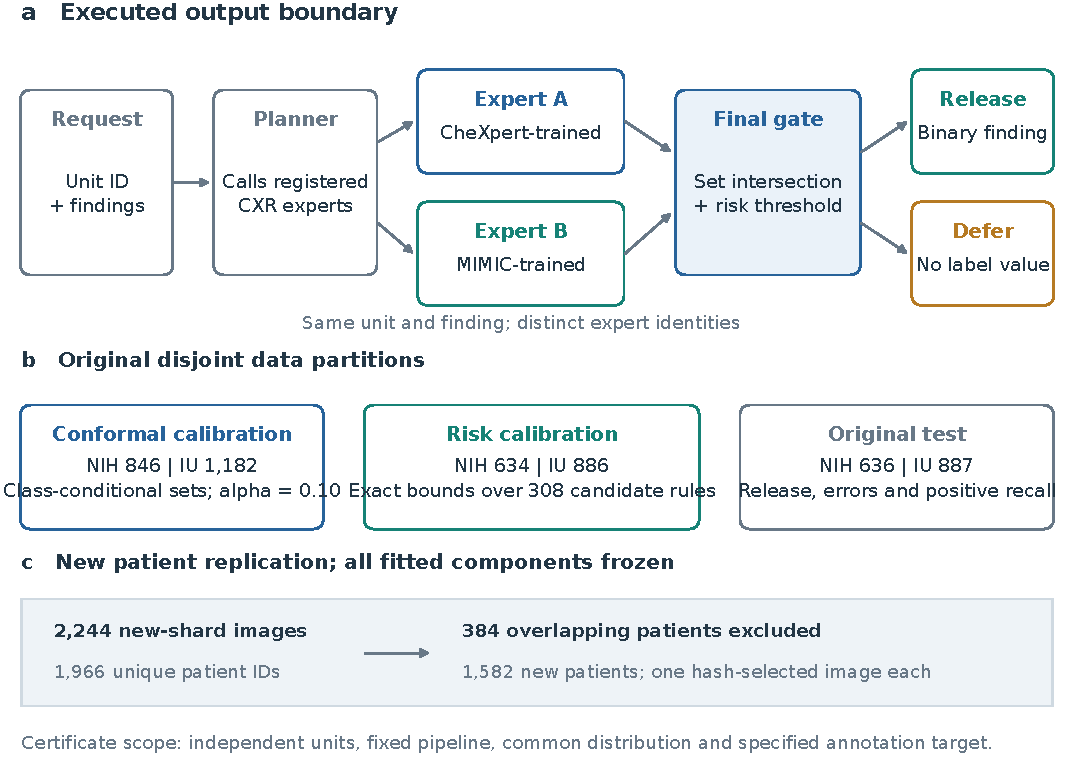
\includegraphics[width=\linewidth]{figures/fig1_architecture.pdf}
\caption{CC-Arbiter's execution path, calibration partitions and new-patient replication. The final gate returns structured binary findings or deferrals. A planner may schedule registered tools, but its free-text response is not the released finding. Both experts must concern the same unit and finding. All original NIH patients, including calibration patients, were excluded from the replication. Fitted models and gates remained frozen.}\label{fig:arch}
\end{figure}

\subsection{Independent calibration of conditional error}
For a fixed finding and threshold $t$, let $A_j(x;t)$ indicate that the proposal is eligible and $u_j(x)\leq t$. The target quantity is
\begin{equation}
R_j(t)=\Pr\{\widehat Y_j\ne\widetilde Y_j\mid A_j(X;t)=1\},
\label{eq:risk}
\end{equation}
when the conditioning event has positive probability. This is distinct from $\Pr\{\widehat Y_j\ne\widetilde Y_j, A_j=1\}$, which can be small solely because release is rare.

The threshold grid $T=\{0,0.05,\ldots,0.50\}$ was fixed before evaluation. For each proposal policy, label and threshold, the independent risk-calibration split yields $N_j(t)$ accepted units and $E_j(t)$ annotation errors. We used the exact one-sided Clopper--Pearson upper bound~\cite{cpinterval}
\begin{equation}
U_j(t)=
\begin{cases}
1, & N_j(t)=0\ \text{or}\ E_j(t)=N_j(t),\\
\operatorname{Beta}^{-1}\!\left(1-\delta/M; E_j(t)+1,N_j(t)-E_j(t)\right), & \text{otherwise},
\end{cases}
\label{eq:bound}
\end{equation}
where $\delta=0.05$ and $M=2\times2\times7\times11=308$ covers the two datasets, two calibrated policies, seven findings and eleven thresholds. For target $r$, the selected threshold is the largest $t$ with $N_j(t)>0$ and $U_j(t)\leq r$. If none qualifies, the finding always defers; zero is not used as a fallback threshold. We evaluated $r\in\{0.05,0.10,0.20\}$ with 0.10 primary. The same simultaneous bounds support all three target choices, so these targets do not create additional threshold families.

Conditional on the independently fitted conformal layer, suppose the risk-calibration and future units are identically distributed and independent. For each fixed candidate rule, the error count conditional on $N_j(t)$ is binomial with parameter $R_j(t)$. The exact upper interval is valid at tail probability $\delta/M$. A union bound gives simultaneous validity for every candidate in the family with probability at least $1-\delta$, allowing selection using the calibration data. Every selected rule then satisfies $R_j(\widehat t_j)\leq r$ on that event. Correlation across labels or experts does not invalidate the union bound; labels are never counted as additional independent binomial trials. The proof is detailed in Additional file~1. Neither monotonic conditional risk nor independence between experts is assumed. The claim is a population bound with calibration confidence, not a per-patient guarantee or a bound on the realized error of every finite test set. For IU, it additionally depends on the unverified independence of reports.

\subsection{Enforced graph execution}
The implemented graph has planning, tool-execution and final-gate nodes (Fig.~\ref{fig:arch}). Methods are registered from the initialized gated class before compilation, avoiding post-compilation class replacement. Evidence is held in invocation state and keyed by request, image or study, finding, and expert identity. Repeated calls overwrite the same expert's evidence; they never count as an additional independent expert. Mismatched image keys, failed calls, nonfinite scores, unsupported tools or missing required findings cannot supply accepted evidence. A failed repeated call invalidates its previous value.

Only the final-gate node creates the returned finding object. Released entries contain binary values; deferred entries contain no finding value and a reason or routing recommendation. A recommendation to obtain another expert or seek review is not evidence that a clinical second pass or human review occurred. We do not certify planner prose, visual question answering, segmentation masks or diagnoses synthesized beyond the seven classifier targets. Thirty-one automated tests, added in three groups as the study was extended, examine statistical edge cases and actual graph behavior, including stale evidence, cross-image mixing, repeated experts, tool failures and attempted planner overrides. The full suite is described in Additional file~1.

We additionally replayed every test unit through the actual LangGraph implementation under two deterministic schedulers: both experts in one round, and one expert per round. Tools returned the newly inferred cached scores without access to reference labels. After the tool calls, each scheduler emitted a deliberate instruction to release every finding as positive. This tested the output boundary rather than language-model reasoning. The designated final object was compared with every offline decision. These replays are software integration evaluations, not end-task LLM accuracy trials or evidence of transfer across agent frameworks.

\subsection{Comparators, outcomes and stress evaluation}
Eight prespecified policies were evaluated on identical test units: always negative; each individual expert at 0.5; mean score at 0.5; agreement of both thresholded experts; conformal singleton intersection without the risk gate; the mean-score risk gate; and CC-Arbiter. With two experts, disagreement is a tie, so the agreement baseline defers rather than fabricating a third vote. The always-negative rule illustrates the effect of class imbalance and was not itself risk-calibrated.

We report release fraction, errors divided by released opportunities, erroneous releases divided by all opportunities, and correctly released positive annotations divided by all positive annotations. The last outcome is positive recall after deferral, so rejected positives count as not recovered. Conditional error is undefined when no predictions are released. Counts are presented by finding, with pooled summaries treated as descriptive. Confidence intervals for pooled quantities use 2,000 bootstrap resamples of independent units, retaining all seven labels together, with seed 718. They condition on the fitted policy; they do not include calibration-set variability. Paired differences use the same resampled units. We make no equivalence or noninferiority claim and did not select thresholds from these intervals.

To test failure mechanisms, a uniform random number was assigned to every test unit with seed 1309. At requested corruption rates of 10\%, 25\% and 50\%, the entire seven-score vector was transformed to $1-p$ for expert B alone, or for both experts with the same mask. The same masks were used across policies, and no case was selected by correctness or reference label. Calibration remained fixed. These experiments model synthetic tool-output failures; the clean-data certificate does not cover the resulting changed score distribution.

\subsection{Secondary comparisons and newly acquired patient replication}
After inspecting the original test results, we fixed a separate, hashed enhancement protocol before acquiring additional NIH data. Analyses on the original test sets are therefore secondary and exploratory. We added two mean-score thresholds per finding: one maximizing Youden's sensitivity plus specificity minus one, and one minimizing empirical classification error. Both used only the original conformal-calibration units, with exact score candidates and ties resolved toward the largest threshold. Neither used risk-calibration or test labels. These baselines have no conditional-risk certificate and do not alter the original family of 308 candidates.

To assess the contribution of rejection, we also matched CC-Arbiter's 10\% policy release count separately for each finding. The alternatives ranked units by distance of their mean score from 0.5 or from the calibration-only Youden threshold, using the corresponding binary prediction. Ties used a hash of unit ID. The resulting batch masks use no reference labels. They are retrospective, cohort-dependent comparisons, not certified deployment policies. Paired bootstrap intervals condition on the fitted thresholds and selected masks. Finding-specific AUROC and average precision (AP), with pointwise 95\% intervals from 2,000 unit bootstrap samples, describe discrimination separately from operating-point performance. Additional file~1 specifies undefined resamples, thresholds and denominators.

We acquired the two prespecified public NIH parquet test shards, numbered 0 and 1, from the \texttt{BahaaEldin0/NIH-Chest-Xray-14} mirror, recording an immutable conversion commit and file hashes. Their 2,244 image records represented 1,966 patients. Excluding all 384 patients shared with the original NIH cohort removed 502 records. Hash-based selection of one image per remaining patient removed 160 additional views, leaving 1,582 patients with no overlap of patient IDs or selected image hashes. Both frozen experts, preprocessing, original NIH conformal quantiles and risk-gate states were reused without refitting. Secondary baseline thresholds also remained fixed. This is newly evaluated, patient-disjoint same-source replication; the data themselves were collected previously. It is not external-center or prospective clinical validation. Certificate transfer still requires a common sampling distribution, which patient disjointness alone cannot establish.

\subsection{Separate positive-sensitive review-routing study}
After the original and replication results were known, a further protocol was locked before acquiring four additional NIH shards. This extension changes the action and estimand: it flags a patient for review rather than releasing a positive diagnosis. Let $Z=1$ denote at least one of the seven annotations, and $F_t=1$ denote a review flag. We separately constrain $\Pr(F_t=0\mid Z=1)$ and $\Pr(Z=1\mid F_t=0)$ to at most 0.10. The former limits missed annotation-positive patients; the latter limits their proportion among unflagged patients. Neither is the original finding-release risk, and an unflagged patient is not declared clinically normal.

Two scores were fixed: a primary logistic stacker of the 14 expert scores, fitted only on the original 846 NIH conformal-calibration patients, and the maximum of the seven expert-mean scores. The additional 4,484 source images represented 3,518 patients. Excluding 961 patients present in either prior NIH cohort and selecting one image per remaining patient yielded 2,557 patients. A fixed random split assigned 1,278 to routing-risk calibration and 1,279 to testing, with no patient or selected-image overlap with previous cohorts. Both one-sided exact binomial bounds use $\delta=0.05$ and a separate family of $2\times41\times2=164$ score--threshold--endpoint combinations. The largest threshold meeting both constraints is selected on calibration only; otherwise all patients are flagged. A distinct final graph node enforces the review action and never supplies a diagnosis value. Additional file~1 specifies fitting, bounds, resampling and execution checks. This is a separate same-source annotation study, not an end-to-end clinical review trial.

\subsection{Use of large language models}
OpenAI Codex was used to revise code, execute the analyses, prepare programmatically generated figures and draft text. It did not generate or adjudicate any reference label, did not determine any released finding, and formed no part of the evaluated system: the released decisions come from the deterministic gate described above. Every reported quantity can be recomputed from the frozen scores in the shared archive, and the authors reviewed and approved the final content.

\section{Results}
\subsection{Coverage and informative evidence}
NIH testing comprised 636 independent patient units and 4,452 label opportunities; IU testing comprised 887 report units and 6,209 opportunities. There were 232 and 193 positive annotation targets, respectively. Across the seven labels, the CheXpert-trained and MIMIC-trained experts had NIH pooled set coverages of 89.1\% and 90.3\%, with mean set sizes of 1.55 and 1.68. IU coverages were 90.1\% and 89.9\%, with mean sizes of 1.77 and 1.73 (Fig.~\ref{fig:coverage}). These pooled quantities do not establish simultaneous or class-wise coverage. Finding-specific denominators and positive/negative coverage are provided in Additional file~1.

Rare classes impose direct limitations on informativeness. For example, only eight IU conformal-calibration reports had a pneumothorax term. At $\alpha=0.10$, the required ninth order statistic is unavailable, so the positive-class threshold becomes infinite. This behavior preserves conservative inclusion of that annotation class, but can prevent a useful negative singleton. Broad sets are therefore an expected consequence of limited calibration support, not evidence that the tool can be safely trusted or that a distribution shift has been detected.

\begin{figure}[htbp]
\centering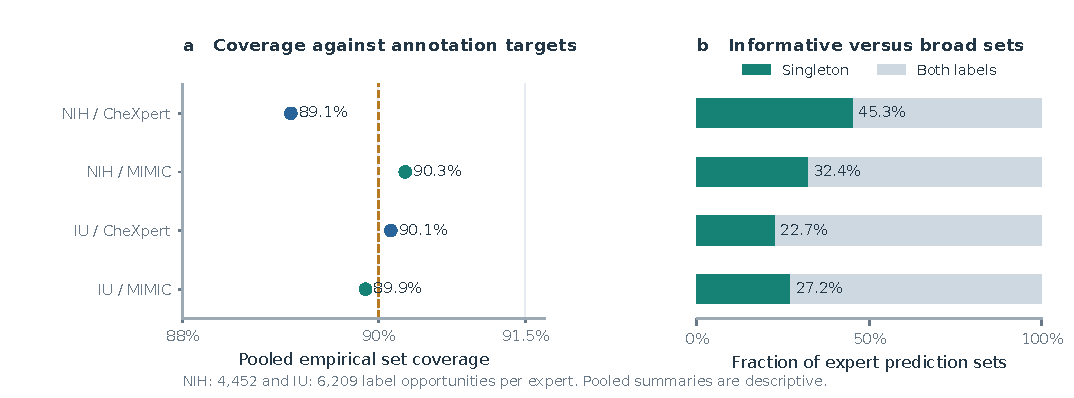
\includegraphics[width=\linewidth]{figures/fig2_coverage.pdf}
\caption{Empirical set coverage and informativeness of the two frozen experts. The dashed vertical line denotes nominal coverage for the class-conditional construction. Pooled coverage is shown descriptively; per-label class counts and coverage are in Additional file~1. There were no empty individual expert sets on these test units. A broad set contains both annotation labels.}\label{fig:coverage}
\end{figure}

\subsection{Selective error and useful release}
At the primary 10\% risk target, CC-Arbiter certified thresholds for three NIH findings: cardiomegaly, consolidation and pneumothorax. The other four findings always deferred. It released 407 of 4,452 opportunities (9.1\%; bootstrap 95\% CI, 8.1--10.2\%), with 10 annotation errors (2.5\% of releases; 95\% CI, 1.1--4.1\%). In comparison, the mean-score risk gate released 1,061 opportunities (23.8\%), with 45 errors (4.2\%). Thus, adding the conformal-intersection requirement reduced both release and erroneous release. The paired decrease in erroneous releases per all opportunities was 0.79 percentage points (95\% CI, 0.54--1.06), accompanied by a 14.69-point decrease in release (95\% CI, 13.93--15.48). This is a rejection trade-off, not evidence of superior diagnostic performance at matched release.

\begin{table}[htbp]
\centering\small\setlength{\tabcolsep}{4pt}
\caption{Primary test results at the 10\% target for the two calibrated gates. Other policies are fixed comparators without this calibration guarantee. TP denotes correctly released positive annotation targets. A dash indicates undefined conditional error.}\label{tab:main}
\begin{tabular}{llrrrr}
\toprule
Dataset & Policy & Release (\%) & Errors / released & Risk (\%) & TP / positives\\
\midrule
NIH & Always negative & 100.0 & 232 / 4452 & 5.2 & 0 / 232\\
NIH & CheXpert expert & 100.0 & 1863 / 4452 & 41.8 & 172 / 232\\
NIH & MIMIC expert & 100.0 & 2599 / 4452 & 58.4 & 201 / 232\\
NIH & Mean score & 100.0 & 1722 / 4452 & 38.7 & 175 / 232\\
NIH & Expert agreement & 70.4 & 1573 / 3136 & 50.2 & 163 / 232\\
NIH & CP intersection & 55.1 & 708 / 2454 & 28.9 & 95 / 232\\
NIH & Risk gate (mean) & 23.8 & 45 / 1061 & 4.2 & 4 / 232\\
NIH & CC-Arbiter & 9.1 & 10 / 407 & 2.5 & 3 / 232\\
\midrule
IU & Always negative & 100.0 & 193 / 6209 & 3.1 & 0 / 193\\
IU & CheXpert expert & 100.0 & 4787 / 6209 & 77.1 & 184 / 193\\
IU & MIMIC expert & 100.0 & 5693 / 6209 & 91.7 & 193 / 193\\
IU & Mean score & 100.0 & 4798 / 6209 & 77.3 & 188 / 193\\
IU & Expert agreement & 78.4 & 4570 / 4869 & 93.9 & 184 / 193\\
IU & CP intersection & 41.0 & 1059 / 2548 & 41.6 & 69 / 193\\
IU & Risk gate (mean) & 5.2 & 7 / 322 & 2.2 & 0 / 193\\
IU & CC-Arbiter & 0.0 & 0 / 0 & -- & 0 / 193\\
\bottomrule
\end{tabular}
\end{table}

On IU, none of the CC-Arbiter candidate thresholds met the required upper bound, and no finding was released. Its observed erroneous-release frequency is zero because all outputs are deferred; its conditional error is undefined. The mean-score gate released 322 of 6,209 opportunities (5.2\%), with seven errors (2.2\% of releases). Figures~\ref{fig:main} and~\ref{fig:cert} show the simultaneous calibration constraints and the resulting coverage of outputs. Increasing the target to 20\% increased NIH CC-Arbiter release to 16.3\%, but IU remained entirely deferred. At the 5\% target, NIH release was 3.1\% with no errors in 137 releases; this observation is not a zero-risk guarantee.

\begin{figure}[htbp]
\centering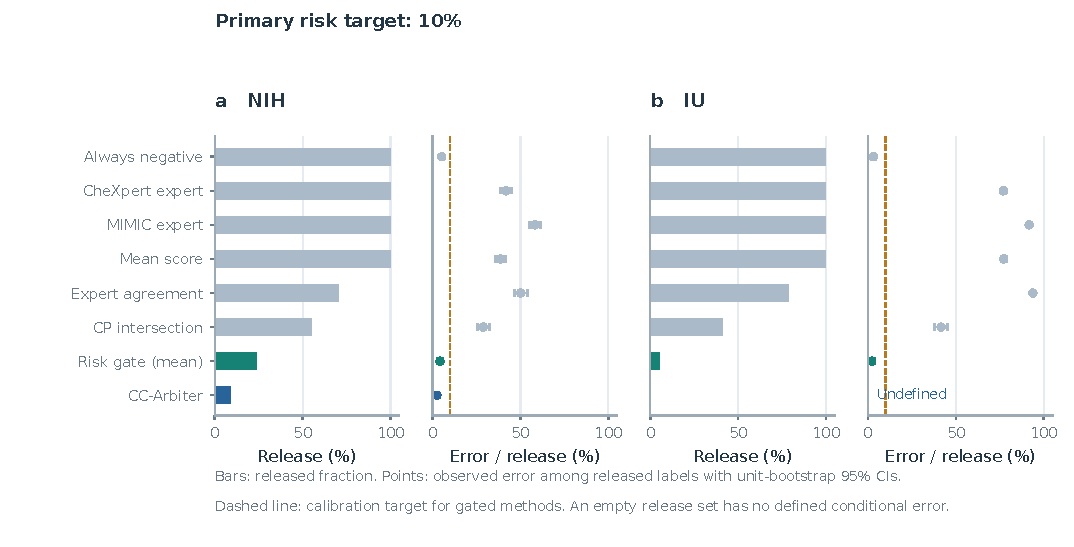
\includegraphics[width=\linewidth]{figures/fig3_selective_performance.pdf}
\caption{Release and empirical conditional error for all prespecified policies. Error intervals resample patients for NIH and reports for IU, keeping correlated labels together. A small error estimate must be interpreted with the associated release fraction and positive retention. The 10\% reference line is the calibration target of the two gated methods; it does not impose a bound on the uncalibrated comparators.}\label{fig:main}
\end{figure}

\begin{figure}[htbp]
\centering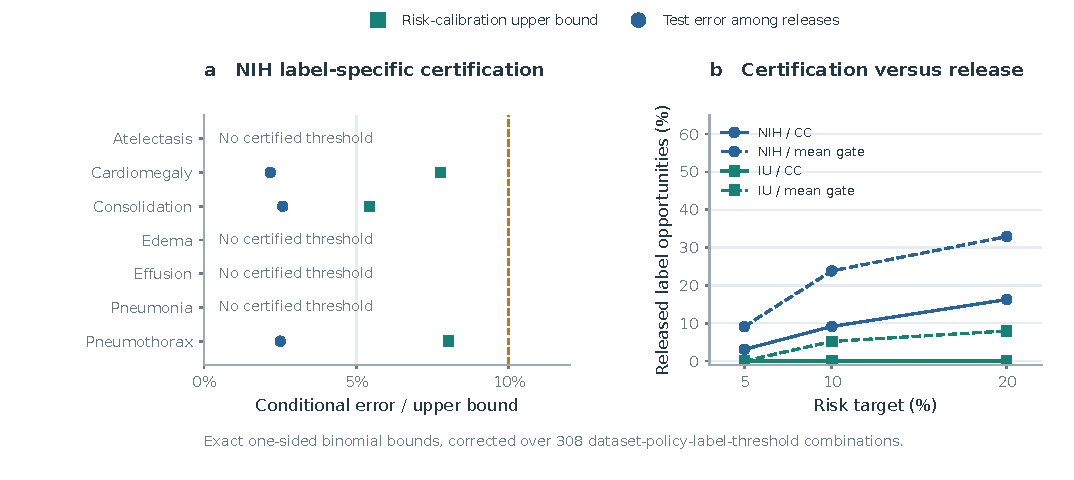
\includegraphics[width=\linewidth]{figures/fig4_risk_certificates.pdf}
\caption{Label-wise certification and its release cost. (a) NIH upper bounds on the independent risk-calibration split and observed test error for the selected CC-Arbiter thresholds. Labels without a qualifying threshold always defer. (b) Released opportunities across the three prespecified targets. Thresholds are selected using calibration only. The IU CC-Arbiter line remains at zero; no conditional-risk estimate is assigned to those empty release sets.}\label{fig:cert}
\end{figure}

The ungated experts and their mean performed poorly against these annotation targets. In particular, mean-score error was 38.7\% on NIH and 77.3\% on IU; simple agreement did not eliminate the high error (Table~\ref{tab:main}). These are properties of the specified released models, normalization, cohort subsets, view aggregation and targets. They should not be generalized to optimized classifiers or to the underlying datasets as a whole.

Class imbalance changes the interpretation of small overall error. An always-negative rule released every opportunity and had empirical error of 5.2\% on NIH and 3.1\% on IU, while recovering no positives. CC-Arbiter correctly released only 3 of 232 NIH positive targets (1.3\%); the mean-score gate recovered 4 (1.7\%). Both recovered no IU positives. Figure~\ref{fig:positive} makes this loss explicit. The observed risk reduction largely reflects withholding outputs and retaining negative annotations. It does not establish a clinically useful screening, triage or diagnostic system.

The low pooled error also did not imply a high positive predictive value. Of CC-Arbiter's eleven positive releases in the original NIH test, three matched the annotation (27.3\%); in the new patients, eight of 26 did (30.8\%). Table~\ref{tab:outcomes} gives the full decomposition of released cells together with the deferred counts. The 232 and 507 positive targets correspond to 172 and 382 patients with at least one positive annotation, so positive-label counts are not independent patient counts.

\begin{table}[htbp]
\centering\small\setlength{\tabcolsep}{5pt}
\caption{CC-Arbiter at the 10\% target, decomposed by released cell and deferral. Counts are label opportunities against the dataset annotations; PPV denotes positive predictive value. Deferred labels receive no finding value.}\label{tab:outcomes}
\begin{tabular}{lrrrrrrrr}
\toprule
Cohort & TP & FP & TN & FN & Deferred positive & Deferred negative & PPV (\%) & Positive recall (\%)\\
\midrule
NIH original test & 3 & 8 & 394 & 2 & 227 & 3,818 & 27.3 & 1.3\\
NIH new patients & 8 & 18 & 1,164 & 5 & 494 & 9,385 & 30.8 & 1.6\\
IU test & 0 & 0 & 0 & 0 & 193 & 6,016 & -- & 0.0\\
\bottomrule
\end{tabular}\par\vspace{3pt}
\noindent\footnotesize TP, FP, TN and FN count released label opportunities only; deferred labels are listed separately and receive no finding value. All comparisons are against the dataset annotations. The dash marks an undefined value when nothing is released.

\end{table}

\begin{figure}[htbp]
\centering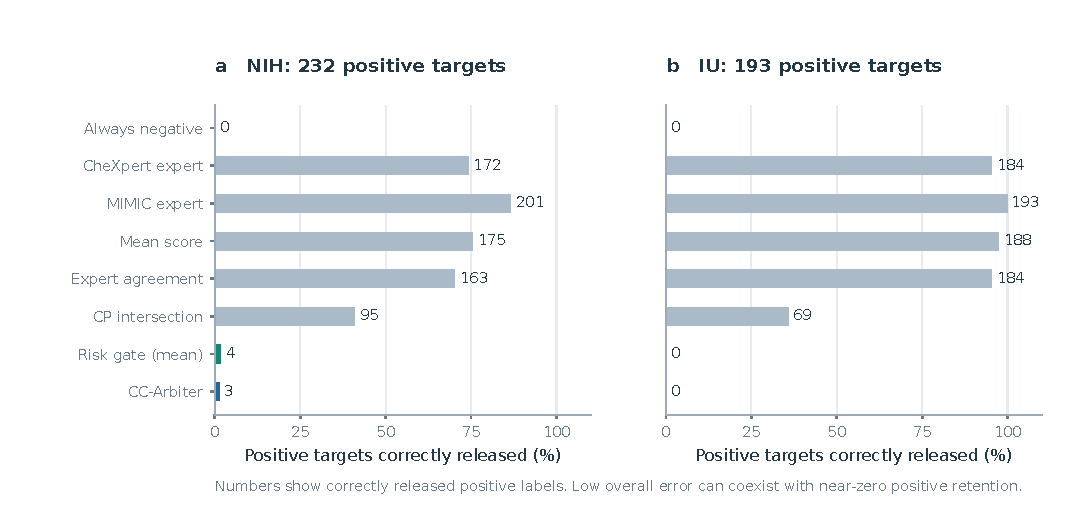
\includegraphics[width=\linewidth]{figures/fig5_positive_retention.pdf}
\caption{Positive annotation targets correctly released after deferral. Numbers next to bars give true-positive counts; the denominators are 232 NIH and 193 IU positive label opportunities. This outcome includes deferral as a failure to recover the positive target. Low pooled conditional error alone can conceal near-total loss of positive findings.}\label{fig:positive}
\end{figure}

\subsection{Correlated failures and execution fidelity}
For NIH, the requested 10\%, 25\% and 50\% masks affected 61, 145 and 325 of 636 patients. With expert B alone flipped, CC-Arbiter released 378, 328 and 238 opportunities, with 10, 10 and 6 errors, respectively. Its released error remained between 2.5\% and 3.0\%, but release decreased. These results are empirical behavior under one corruption mechanism, not an attack guarantee.

Shared corruption had a different effect. Flipping both experts for 61 patients produced 75 errors in 436 released opportunities (17.2\%). At 145 and 325 corrupted patients, error rose to 35.7\% and 62.1\%, respectively (Fig.~\ref{fig:stress}). Correlated incorrect evidence can remain mutually compatible, and clean calibration does not control its changed risk. The experiment therefore rejects a general claim of complete failure containment. IU CC-Arbiter retained its all-defer behavior because it had no certified clean threshold.

\begin{figure}[htbp]
\centering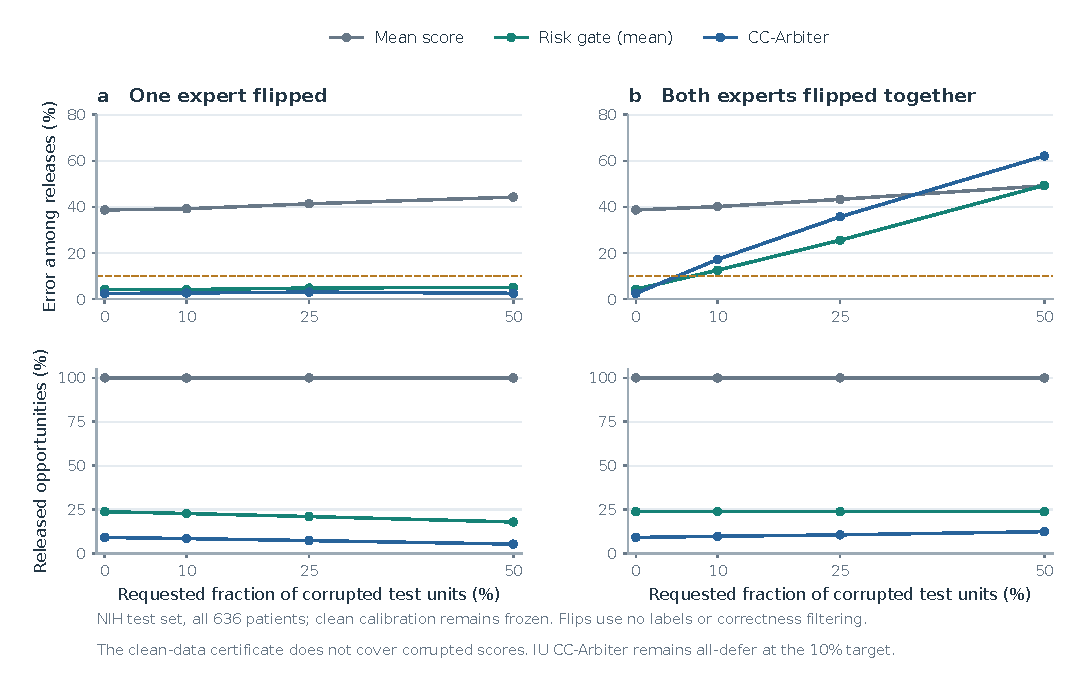
\includegraphics[width=\linewidth]{figures/fig6_correlated_failures.pdf}
\caption{NIH failure stress tests with all patients retained and identical label-independent masks across policies. The horizontal reference is the clean-data calibration target, which is not guaranteed under these corruptions. Unilateral corruption mainly reduces release, whereas shared corruption can generate confident, mutually consistent errors. The score transformation is applied at the tool-output level and does not represent a specific clinical acquisition shift.}\label{fig:stress}
\end{figure}

All 31 original and added automated tests passed. Replaying 3,105 test units, including the new NIH patients, under each of the two scheduling patterns produced 6,210 graph invocations and 43,470 final label decisions, with zero discrepancies against offline CC-Arbiter. Each invocation recorded both distinct expert outputs; deliberately conflicting planner prose did not replace the final structured decisions. Median replay time across cohorts and schedulers was approximately 1.1--2.4 ms per unit, excluding model inference and language-model calls. This verifies the implemented output boundary under the tested conditions, not negligible overhead or clinical accuracy in an end-to-end agent deployment.

\subsection{Secondary operating-point audit and patient replication}
Threshold-free discrimination was better than the poor fixed-threshold errors alone suggest (Fig.~\ref{fig:discrimination}). Mean-score AUROC ranged from 0.672 to 0.839 across findings in the original NIH test, 0.538 to 0.781 in IU, and 0.673 to 0.873 in the new NIH patients. AP and positive denominators are reported in Additional file~1; rare IU targets have especially wide uncertainty. This discrimination does not establish probability calibration or an adequate clinical operating point.

Using only conformal-calibration units to choose Youden thresholds yielded original NIH and IU mean-score errors of 41.5\% and 29.9\%, respectively, recovering 183/232 and 87/193 positive targets at full release. Thus, threshold tuning substantially improved IU performance but did not improve the NIH unweighted error. Thresholds chosen instead to minimize calibration error produced test errors of 5.2\% and 3.2\%, but recovered only two and three positive targets. These opposing outcomes illustrate the importance of defining the utility of positive findings before optimizing a threshold. They also rule out interpreting the original 0.5 baseline as the strongest possible ungated classifier.

\begin{figure}[htbp]
\centering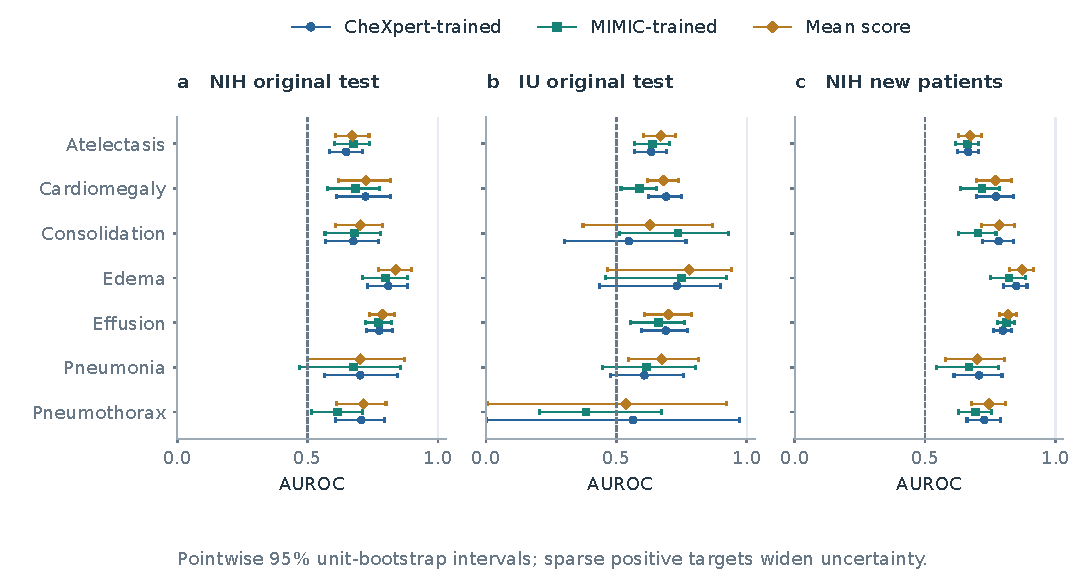
\includegraphics[width=\linewidth]{figures/fig7_discrimination.pdf}
\caption{Secondary audit of discrimination in original and new test cohorts. AUROC and pointwise 95\% intervals use unit bootstrap resampling, preserving within-unit label correlation. Intervals do not correct for comparisons across findings or models and are not used to select a policy. The vertical reference denotes AUROC 0.5. AP, positive counts and valid bootstrap counts are supplied separately.}\label{fig:discrimination}
\end{figure}

The 1,582 new NIH patients contributed 11,074 opportunities and 507 positive targets. Without recalibration, CC-Arbiter released 1,195 opportunities (10.8\%; 95\% CI, 10.1--11.5\%), with 23 errors (1.9\%; 95\% CI, 1.1--2.8\%) and eight positives recovered (1.6\% of positive targets). The mean-score risk gate released 2,949 opportunities with 91 errors and 11 recovered positives (Table~\ref{tab:replication}). The new-patient results reproduce the low-release, low-positive-retention pattern, while remaining subject to the annotation and source-sampling limitations.

\begin{table}[htbp]
\centering\small\setlength{\tabcolsep}{4pt}
\caption{Frozen-policy replication in 1,582 new NIH patients: 11,074 label opportunities and 507 positive targets. TP and recall concern correctly released positive annotations. Gates use the original 10\% target. Matched rules share CC-Arbiter's release count for every finding, use no new target labels for selection and have no risk certificate.}\label{tab:replication}
\begin{tabular}{lrrrrr}\toprule
Policy & Released & Errors & Error (\%) & TP & Recall (\%)\\\midrule
Always negative & 11,074 & 507 & 4.6 & 0 & 0.0 \\
Mean at 0.5 & 11,074 & 3,636 & 32.8 & 377 & 74.4 \\
Mean: calibration Youden & 11,074 & 3,842 & 34.7 & 394 & 77.7 \\
Mean: calibration min. error & 11,074 & 518 & 4.7 & 5 & 1.0 \\
Mean risk gate & 2,949 & 91 & 3.1 & 11 & 2.2 \\
CC-Arbiter & 1,195 & 23 & 1.9 & 8 & 1.6 \\
Mean: matched release & 1,195 & 14 & 1.2 & 3 & 0.6 \\
Youden: matched release & 1,195 & 123 & 10.3 & 25 & 4.9 \\
\bottomrule\end{tabular}

\end{table}

At identical per-label release counts, simple mean-score ranking produced five errors among 407 original NIH releases and 14 among 1,195 new-patient releases, versus CC-Arbiter's 10 and 23 errors (Fig.~\ref{fig:matched}). The CC-minus-ranking conditional-error differences were 1.23 percentage points (paired 95\% CI, 0.28--2.41) and 0.75 points (0.09--1.50), conditional on the fitted thresholds and chosen batch masks. Ranking recovered fewer positives: zero versus three originally, and three versus eight in replication. Youden-based matched ranking recovered more positives (six and 25) but incurred more errors (50 and 123). These are descriptive trade-offs, not a multiplicity-adjusted superiority trial. IU had no nonzero CC-Arbiter release budget, so a matched-release conditional-error comparison was undefined.

\begin{figure}[htbp]
\centering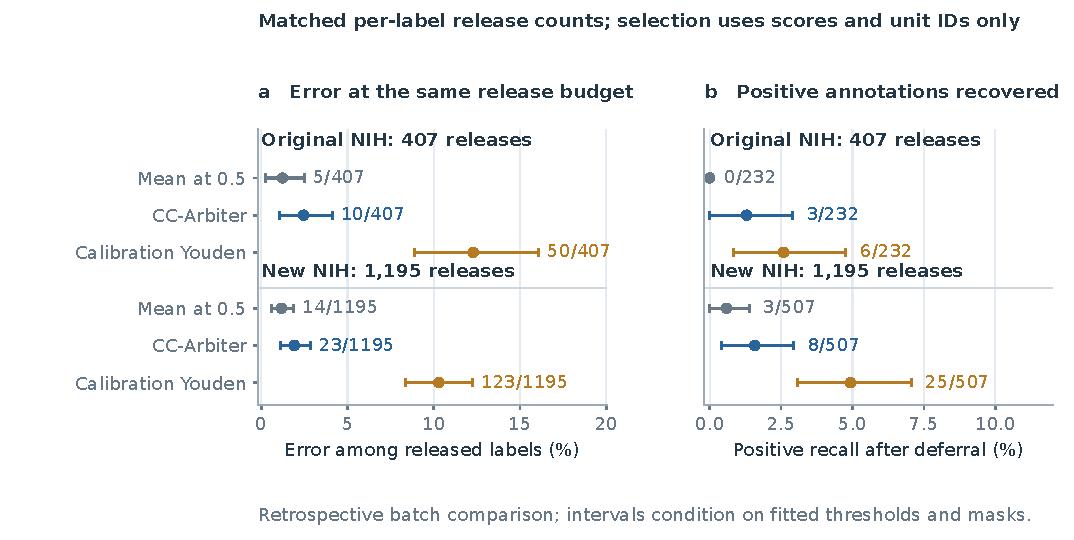
\includegraphics[width=\linewidth]{figures/fig8_matched_replication.pdf}
\caption{Error and positive recall at exactly matched per-finding release counts in two disjoint NIH test cohorts. Mean and Youden ranking select by distance from the corresponding score threshold; ties use a hash of unit ID. Points and intervals use the same patient bootstrap samples, conditional on the observed batch selections. Numerators and denominators are shown explicitly. No comparator uniformly improves both error and positive retention.}\label{fig:matched}
\end{figure}

\subsection{Post hoc projection-stratified audit}
After the primary results were known, we additionally tabulated release, error and positive recovery separately for anteroposterior (AP) and posteroanterior (PA) examinations in both NIH cohorts. Policies, thresholds, calibration states and the reference annotations were unchanged. In the original NIH test, CC-Arbiter released 42 of 1,610 AP opportunities (2.6\%) with seven errors among releases (16.7\%; pointwise patient-bootstrap 95\% CI, 6.3--29.4\%) and 365 of 2,842 PA opportunities (12.8\%) with three errors (0.8\%; 95\% CI, 0.0--1.9\%). The new-patient cohort showed the same ordering: 122 of 3,717 AP opportunities (3.3\%; 5.7\% error; 95\% CI, 1.8--10.1\%) and 1,073 of 7,357 PA opportunities (14.6\%; 1.5\%; 95\% CI, 0.7--2.4\%) (Table~\ref{tab:subgroups}). These analyses were not prespecified and were not adjusted for differences in patient or released-label composition; they carry no projection-specific risk guarantee, and the AP intervals are wide because few labels were released there.

\begin{table}[htbp]
\centering\footnotesize\setlength{\tabcolsep}{3.5pt}
\caption{Post hoc projection-stratified audit in both NIH cohorts with all policies frozen. Intervals are pointwise patient-bootstrap percentile intervals within each stratum and are not multiplicity-adjusted or calibrated as subgroup guarantees.}\label{tab:subgroups}
\begin{tabular}{llrrrrrr}
\toprule
Cohort & Projection & Patients & Released / opportunities & Release (\%) & Errors / released & Error (\%) [95\% CI] & TP / positives\\
\midrule
NIH original test & AP & 230 & 42 / 1,610 & 2.6 & 7 / 42 & 16.7 [6.3, 29.4] & 1 / 102\\
NIH original test & PA & 406 & 365 / 2,842 & 12.8 & 3 / 365 & 0.8 [0.0, 1.9] & 2 / 130\\
NIH new patients & AP & 531 & 122 / 3,717 & 3.3 & 7 / 122 & 5.7 [1.8, 10.1] & 3 / 239\\
NIH new patients & PA & 1,051 & 1,073 / 7,357 & 14.6 & 16 / 1,073 & 1.5 [0.7, 2.4] & 5 / 268\\
\bottomrule
\end{tabular}\par\vspace{3pt}
\noindent\footnotesize Conditional error is undefined for a stratum with no releases; both strata released labels here. Percentile intervals use 2,000 patient bootstrap resamples within each stratum and retain all seven labels per sampled patient.

\end{table}

\subsection{Certification feasibility}
For a candidate with zero observed errors, the exact upper bound is $1-(\delta/M)^{1/n}$. Therefore, at least 171, 83 and 40 accepted risk-calibration units are necessary to certify targets of 5\%, 10\% and 20\%, respectively; any observed errors raise the requirement. These are accepted counts for one fixed candidate, not total cohort sizes or counts pooled across findings. For IU at 10\%, each finding had at least one candidate with 83 or more accepted units, yet no candidate met the error bound. Sample scarcity alone therefore does not explain its all-defer result. Minimum candidate upper bounds ranged from 0.318 to 1.000, compared with 0.046 to 0.239 for NIH. Full counts and bounds are in Additional file~1.

\subsection{Positive attrition and review-routing feasibility}
The original NIH mean-score rule correctly released 175 of 232 positive annotations, the conformal intersection 95, and CC-Arbiter only three (Fig.~\ref{fig:review}a). Moreover, only three of CC-Arbiter's eleven positive releases matched the positive annotation, illustrating that its low pooled error does not imply high positive predictive value. In IU the corresponding correct-positive counts were 188, 69 and zero. The intersection and the risk gate both contribute to positive loss; these summaries do not imply that the intermediate positive sets are nested.

The separate routing-calibration set contained 250 annotation-positive patients. Neither score had a threshold satisfying both 10\% upper bounds (Fig.~\ref{fig:review}b). The minimum upper bound on positivity among unflagged patients was 12.7\% for stacking and 11.6\% for maximum mean, already exceeding the target. Consequently, both selected policies flagged all 1,279 test patients, including all 267 annotation-positive patients. This is the structural all-flag fallback, not an improvement in automatic positive diagnosis, and it reduces no review flags. Fixed 0.5 comparators illustrate the opposing error: the stacker flagged only 73/267 positive patients and maximum mean 216/267, without the specified certificates. Their full counts are in Additional file~1. No actual human reviews or clinical workload savings were measured.

\begin{figure}[htbp]
\centering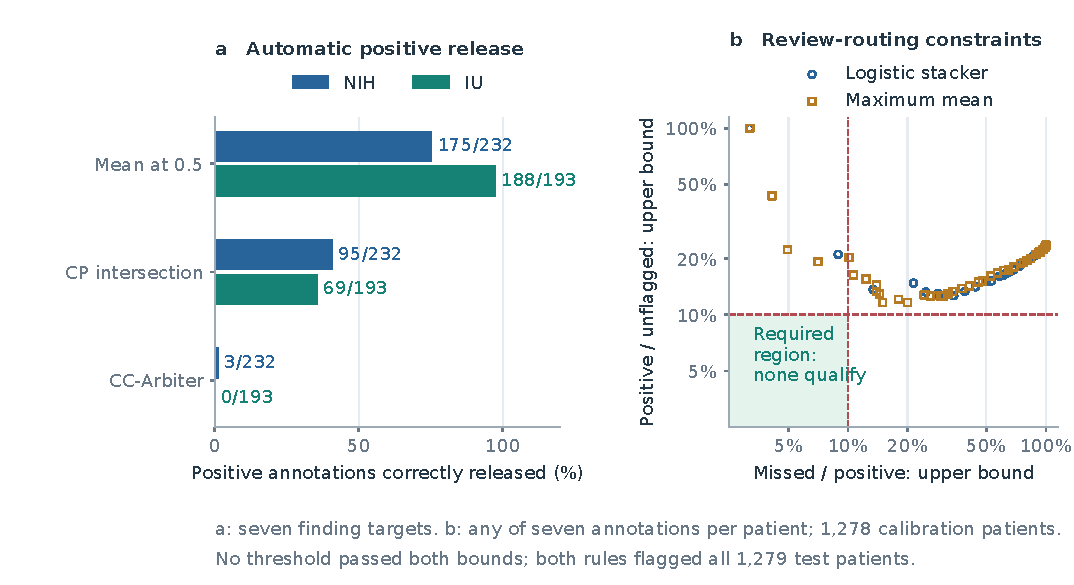
\includegraphics[width=\linewidth]{figures/fig9_positive_review.pdf}
\caption{Positive loss and the feasibility of a separate review action. (a) Correctly released positive annotations in the original tests; the methods are not assumed to form nested positive subsets. (b) Simultaneous exact calibration bounds for 41 thresholds under each of two routing scores. The shaded region requires both bounds at most 10\%; no candidate falls inside it. Axes in panel b are logarithmic. The calibration unit and target differ from panel a: patients with any of seven annotations. All-flag routing does not constitute automatic diagnosis or measured workload reduction.}\label{fig:review}
\end{figure}

\section{Discussion}
This study separates three often conflated properties: calibrated set inclusion, conditional-risk selection, and software enforcement. Individual conformal sets can have coverage close to nominal while their singleton intersection has high selective error. A separately calibrated gate can limit that error while retaining very little evidence. A final graph node can enforce the resulting rule even when the planner proposes a different answer. None of these properties establishes the clinical value of the released findings.

The comparisons with simpler selection are central. Both calibrated gates use the same independent calibration split, candidate thresholds and family correction; the mean-score gate released more labels. At identical per-label budgets, mean-score ranking incurred fewer errors than CC-Arbiter in both NIH cohorts, although it also recovered fewer positives. The conformal-intersection stage is therefore not established as necessary or more efficient. Its role here is to make evidence compatibility explicit. The separately locked new-patient replication strengthens the evidence for this trade-off without converting the secondary original-test analyses into prespecified primary findings.

The all-negative comparator further limits interpretation. With positive annotation rates of only 5.2\% and 3.1\%, unweighted error is an incomplete clinical objective. Our exact bounds control that defined error, but they do not constrain sensitivity, false-negative risk within positive cases, or the clinical cost of missed disease. A system that refuses nearly every positive output cannot be justified by a small pooled error alone. Useful extensions would prespecify class-sensitive losses or simultaneous sensitivity and predictive-value requirements, using enough independently labelled positive cases to calibrate them. Optimizing such requirements after viewing these test results would require a new validation set.

Correlated failure is another boundary. Experts trained on different sources still share an architecture and can fail together. Intersected sets check compatibility rather than truth; they can agree on an incorrect label. We did not assume expert independence in the proof, but the proof does require calibration and future units to follow the same pipeline and distribution. Our corruption changes that distribution. The observed increase to 17.2\% error after joint flips in 9.6\% of NIH patients is therefore consistent with the guarantee's stated domain and shows why it must not be presented as adversarial robustness.

Several limitations affect external validity. The NIH analyses used two original shards, two additional shards for the frozen-policy replication and four further shards for the separate review-routing study, with one hash-selected image per patient throughout. All three patient cohorts were disjoint in the available identifiers and selected-image hashes. They came from the same source, so they do not provide external-centre validation. IU images form a locally available subset, and report-level aggregation includes lateral views. Stable cross-report patient identifiers are unavailable. The secondary threshold audit changes operating points but neither retrains experts nor calibrates their scores as disease probabilities. Label rarity can make conformal thresholds infinite and exact risk bounds conservative, while observed errors can independently prevent certification even when accepted counts are adequate. The study uses text-mined or report-indexing targets without new radiologist adjudication. An error against those targets need not be a clinical error, and agreement need not be clinical correctness. Bootstrap intervals condition on fitted calibration layers and do not capture their sampling variability. Results concern the specified processing and annotation task rather than diagnostic deployment.

Our bounds were calibrated by finding within each data source and were not conditioned on projection, age or the recorded sex field. The post hoc AP/PA differences therefore describe where released outputs occurred rather than a calibrated subgroup guarantee, and they may reflect differences in patient and released-label composition as well as projection-related model behaviour.

The Bonferroni-corrected exact procedure is deliberately simple and can be statistically inefficient. The additional routing study also failed to certify a reduction in review flags under the specified dual objective. It does not prove that all routing scores or calibration methods must fail; it shows that these fixed experts, scores, sample sizes and constraints did not suffice. We did not compare the release efficiency of newer selective-risk methods such as SCoRE~\cite{score}; no optimality claim is made. Deterministic graph replay does not evaluate natural language planning, clinical second-pass resolution or actual human review. Better image-model discrimination, clinically adjudicated targets and independently validated utilities remain necessary before claiming useful clinical performance.

\begin{samepage}
\section{Conclusions}
CC-Arbiter makes finite-sample risk calibration and selective output enforcement jointly auditable. Original and replication NIH cohorts showed low conditional error accompanied by extensive rejection and poor positive retention; IU yielded no certified release. Mean-score ranking had fewer errors at matched release counts but retained fewer positives. A separate positive-sensitive routing study also failed to certify a reduction in review flags, while shared expert corruption defeated clean-data control. The findings support reporting assumptions, execution, release, positive retention and action-specific utility together; they establish neither clinical deployment readiness nor a general accuracy advantage.
\end{samepage}

\section*{Abbreviations}
AP: anteroposterior projection (the ranking metric average precision is written in full); AUROC: area under the receiver operating characteristic curve; CI: confidence interval; FN: false negative; FP: false positive; IU: Indiana University chest radiograph collection; LLM: large language model; MeSH: Medical Subject Headings; NIH: National Institutes of Health ChestX-ray14 collection; PA: posteroanterior projection; PPV: positive predictive value; TF32: TensorFloat-32; TN: true negative; TP: true positive.

\section*{Declarations}
\paragraph{Ethics approval and consent to participate.} This work is a secondary computational analysis of two publicly available, de-identified chest radiograph datasets, NIH ChestX-ray14 and the Indiana University collection. No participants were recruited or contacted, no new clinical data were collected, no intervention was performed and no identifiable information is reported. Because the study uses only previously collected, publicly released, de-identified data, ethics approval and participant consent were not required, and no ethics committee reference number applies. Consent and data-use terms for the original collections were administered by the dataset providers. The authors confirmed this determination with the supervising faculty member (X.~Kong, 12 October 2026).
\paragraph{Consent for publication.} Not applicable. No identifiable individual information or participant images are reproduced in this manuscript.
\paragraph{Availability of data and materials.} The datasets analysed are publicly available and fully cited in the reference list: the NIH ChestX-ray14 collection~\cite{nih} and the Indiana University chest radiograph collection~\cite{iu}. Derived files supporting the conclusions, including the frozen split manifests, expert scores, calibrated thresholds, per-unit decisions and machine-readable results, are included within the article's additional files. Project name: CC-Arbiter reproducibility archive. Project home page: https://github.com/binghe-glacier/cc-arbiter; the same archive accompanies this submission as Additional file~2. Archived version: Zenodo, https://doi.org/10.5281/zenodo.23329663. Operating system: platform independent, developed and tested on Windows~11. Programming language: Python (3.11). Other requirements: NumPy, SciPy and Matplotlib for analysis from the supplied scores; LangGraph and LangChain Core for execution replay; PyTorch and TorchXRayVision for optional re-inference, which additionally requires network access to download public model weights. License: MIT. Restrictions for non-academics: none stated beyond the terms of the source datasets. Original radiographs, report text and pretrained weights are not redistributed and remain subject to their providers' terms.
\paragraph{Competing interests.} The authors declare that they have no competing interests.
\paragraph{Funding.} This research received no specific grant from any funding agency in the public, commercial, or not-for-profit sectors.
\paragraph{Authors' contributions.} YY: Conceptualization, Methodology, Software, Formal analysis, Investigation, Data curation, Visualization, Writing (original draft). XK: Supervision, corresponding author.
\paragraph{Acknowledgements.} Not applicable.

\paragraph{Generative AI assistance.} OpenAI Codex assisted with code revision, execution of the analyses, preparation of programmatically generated figures and manuscript drafting. It produced no reference labels and no released findings. The authors are responsible for verifying and approving the final submitted content.
\paragraph{Additional files.} Additional file~1: supplementary methods, statistical proof, cohort composition, post hoc subgroup descriptives, cohort-level positive counts and detailed calibration results (PDF). Additional file~2: reproducibility archive containing executable code, fixed derived scores, split manifests, machine-readable results and provenance records (ZIP). Original images, report text and model weights are excluded from both files.
\begin{thebibliography}{99}
\small
\bibitem{medrax} Fallahpour A, Ma J, Munim A, Lyu H, Wang B. MedRAX: Medical reasoning agent for chest X-ray. 2025. arXiv:2502.02673.
\bibitem{cxragent} Lou J, Yang Y, Yu Z, Fu Z, Han W, Huang Q, Yu J. CXRAgent: Director-orchestrated multi-stage reasoning for chest X-ray interpretation. 2025. arXiv:2510.21324.
\bibitem{radagents} Zhang K, Barrett CD, Kim J, Sun L, Taghavi T, Kenthapadi K. RadAgents: Multimodal agentic reasoning for chest X-ray interpretation with radiologist-like workflows. MIDL 2026. arXiv:2509.20490.
\bibitem{vovk} Vovk V, Gammerman A, Shafer G. Algorithmic learning in a random world. Springer; 2005.
\bibitem{gentle} Angelopoulos AN, Bates S. A gentle introduction to conformal prediction and distribution-free uncertainty quantification. 2021. arXiv:2107.07511.
\bibitem{ltt} Angelopoulos AN, Bates S, Cand\`es EJ, Jordan MI, Lei L. Learn then test: Calibrating predictive algorithms to achieve risk control. 2021. arXiv:2110.01052.
\bibitem{crc} Angelopoulos AN, Bates S, Fisch A, Lei L, Schuster T. Conformal risk control. ICLR 2024. arXiv:2208.02814.
\bibitem{score} Bai T, Jin Y. Conformal selective prediction with general risk control. 2026. arXiv:2603.24704.
\bibitem{coma} Gasparin M, Ramdas A. Conformal online model aggregation. arXiv:2403.15527. Revised 2025.
\bibitem{nih} Wang X, Peng Y, Lu L, Lu Z, Bagheri M, Summers RM. ChestX-ray8: Hospital-scale chest X-ray database and benchmarks on weakly-supervised classification and localization of common thorax diseases. Proceedings of CVPR. 2017. arXiv:1705.02315.
\bibitem{iu} Demner-Fushman D, Kohli MD, Rosenman MB, et al. Preparing a collection of radiology examinations for distribution and retrieval. J Am Med Inform Assoc. 2016;23:304--310. doi:10.1093/jamia/ocv080.
\bibitem{xrv} Cohen JP, Viviano JD, Bertin P, et al. TorchXRayVision: A library of chest X-ray datasets and models. 2021. arXiv:2111.00595.
\bibitem{densenet} Huang G, Liu Z, van der Maaten L, Weinberger KQ. Densely connected convolutional networks. Proceedings of CVPR. 2017. arXiv:1608.06993.
\bibitem{chex} Irvin J, Rajpurkar P, Ko M, et al. CheXpert: A large chest radiograph dataset with uncertainty labels and expert comparison. 2019. arXiv:1901.07031.
\bibitem{mimic} Johnson AEW, Pollard TJ, Berkowitz SJ, et al. MIMIC-CXR, a de-identified publicly available database of chest radiographs with free-text reports. Sci Data. 2019;6:317. doi:10.1038/s41597-019-0322-0.
\bibitem{cpinterval} Clopper CJ, Pearson ES. The use of confidence or fiducial limits illustrated in the case of the binomial. Biometrika. 1934;26:404--413. doi:10.1093/biomet/26.4.404.
\end{thebibliography}
\end{document}
;
% the compact reading version omits it.
\usepackage{setspace}
\renewcommand{\rmdefault}{ptm}
\renewcommand{\sfdefault}{phv}
\renewcommand{\ttdefault}{phv}
% Font setup that compiles under both engines.
% XeTeX/Tectonic: native OpenType Times/Arial declarations, no extra packages.
% pdfLaTeX (used by the journal's TeX Live 2021 build): standard PS fonts.
\ifdefined\XeTeXversion
\DeclareFontFamily{TU}{ccserif}{}
\DeclareFontShape{TU}{ccserif}{m}{n}{<->"[local-fonts/times.ttf]"}{}
\DeclareFontShape{TU}{ccserif}{m}{it}{<->"[local-fonts/timesi.ttf]"}{}
\DeclareFontShape{TU}{ccserif}{b}{n}{<->"[local-fonts/timesbd.ttf]"}{}
\DeclareFontShape{TU}{ccserif}{bx}{n}{<->"[local-fonts/timesbd.ttf]"}{}
\DeclareFontShape{TU}{ccserif}{b}{it}{<->"[local-fonts/timesbi.ttf]"}{}
\DeclareFontShape{TU}{ccserif}{bx}{it}{<->"[local-fonts/timesbi.ttf]"}{}
\DeclareFontFamily{TU}{ccsans}{}
\DeclareFontShape{TU}{ccsans}{m}{n}{<->"[local-fonts/arial.ttf]"}{}
\DeclareFontShape{TU}{ccsans}{b}{n}{<->"[local-fonts/arialbd.ttf]"}{}
\DeclareFontShape{TU}{ccsans}{bx}{n}{<->"[local-fonts/arialbd.ttf]"}{}
\DeclareFontShape{TU}{ccsans}{m}{it}{<->"[local-fonts/ariali.ttf]"}{}
\renewcommand{\rmdefault}{ccserif}
\renewcommand{\sfdefault}{ccsans}
\renewcommand{\ttdefault}{ccsans}
\else
\usepackage[T1]{fontenc}
\usepackage{mathptmx}
\usepackage[scaled=0.92]{helvet}
\renewcommand{\ttdefault}{phv}
\fi

\DeclareMathSizes{12}{10}{7}{5}
\DeclareMathSizes{9}{10}{7}{5}
\makeatletter\renewcommand\normalsize{\@setfontsize\normalsize{12}{15}}\makeatother
\normalsize
\setlength{\textwidth}{166mm}
\setlength{\textheight}{242mm}
\setlength{\oddsidemargin}{-3mm}
\setlength{\evensidemargin}{-3mm}
\setlength{\topmargin}{-15mm}
\setlength{\parskip}{3pt}
\setlength{\parindent}{12pt}
\setlength{\emergencystretch}{2em}
\renewcommand{\baselinestretch}{1.09}
\ifdefined\REVIEWCOPY\usepackage{lineno}\AtBeginDocument{\doublespacing\linenumbers}\fi
\renewcommand{\topfraction}{0.92}\renewcommand{\bottomfraction}{0.85}
\renewcommand{\textfraction}{0.06}\renewcommand{\floatpagefraction}{0.78}
\title{Auditing selective release of chest radiograph findings: retrospective evaluation of CC-Arbiter}
\author{Yaocong Yang and Xiangyong Kong\\[4pt]
\small School of Health Science and Engineering,\\
\small University of Shanghai for Science and Technology, Shanghai, China\\
\small Correspondence: Xiangyong Kong, \texttt{kxy@usst.edu.cn}}
\date{}
\begin{document}
\maketitle
\begin{abstract}
\noindent\textbf{Background:} Low error among selectively released chest radiograph findings can conceal the rejection of nearly all positive findings. We evaluated an executable evidence gate and audited its release, positive retention and failure boundaries.\par
\noindent\textbf{Methods:} CC-Arbiter intersects class-conditional conformal sets from two frozen DenseNet-121 experts and applies independently calibrated conditional-error gates using exact, multiplicity-corrected binomial bounds. The original cohorts comprised 2,116 NIH patients and 2,955 IU reports, with disjoint conformal, risk-calibration and test splits. Seven dataset annotations served as targets, without new clinical adjudication. A secondary protocol added calibration-only threshold baselines, score discrimination and comparisons at matched release counts. Frozen policies were then evaluated in 1,582 additional NIH patients absent from the original cohort. A separate review-routing study used 2,557 additional NIH patients, split into independent risk-calibration and test sets. It constrained both missed positives and positivity among unflagged patients. Projection-stratified results were examined post hoc. Score corruption and graph execution were also assessed.\par
\noindent\textbf{Results:} At the 10\% risk target, CC-Arbiter released 407/4,452 original NIH opportunities (9.1\%), with 10 errors (2.5\%; unit-bootstrap 95\% confidence interval, 1.1--4.1\%) and only 3/232 positive targets recovered. Positive predictive value was 27.3\%. It released nothing on IU. New-patient replication yielded 1,195/11,074 releases (10.8\%), 23 errors (1.9\%; 95\% confidence interval, 1.1--2.8\%), 8/507 positive targets recovered and positive predictive value of 30.8\%. Anteroposterior examinations received fewer and more erroneous releases than posteroanterior ones (originally 2.6\% versus 12.8\% release; 16.7\% versus 0.8\% error). Simple mean-score ranking at identical per-label release counts produced fewer errors in both NIH cohorts (5 and 14), while recovering fewer positives (0 and 3). Calibration-only Youden thresholds reduced IU mean-score error from 77.3\% to 29.9\%. Shared corruption in 61/636 original NIH patients raised CC-Arbiter error to 17.2\%. Both routing procedures flagged all 1,279 new test patients because no threshold met both constraints. All 43,470 original and replication label decisions matched offline gating.\par
\noindent\textbf{Conclusions:} The framework makes risk calibration and output enforcement auditable, but low selective error did not establish useful positive retention or superiority over simpler selection. Replication supports joint reporting of release, positive recall, matched-budget comparisons and correlated failures.
\end{abstract}
\noindent\textbf{Keywords:} chest radiograph; selective prediction; conformal prediction; risk control; medical imaging agents; reproducibility

\section{Background}
Medical imaging agents combine a planning model with specialist tools for image classification, visual question answering, segmentation and report generation. MedRAX introduced a unified chest radiograph tool interface and the ChestAgentBench benchmark~\cite{medrax}. CXRAgent and RadAgents further develop staged verification and radiologist-inspired workflows~\cite{cxragent,radagents}. These systems motivate a practical engineering question: which tool-derived statements may reach the user when experts disagree or provide uncertain evidence? Providing confidence information to a language model and enforcing an output rule are different operations. A model may disregard an uncertainty annotation, and a correctly written monitor may still be absent from the executed graph.

Conformal prediction provides one component of a solution. Given suitable calibration data and exchangeability, it constructs prediction sets with finite-sample coverage~\cite{vovk,gentle}. Coverage concerns whether a set contains the specified target; it does not by itself bound error among the subset of outputs that a system chooses to release. Intersecting multiple sets, selecting a singleton and withholding some predictions introduce further selection. A separate selective-risk argument is therefore needed. Moreover, a guarantee against imperfect dataset annotations does not become a guarantee against clinical diagnoses.

Risk calibration methods address several different objectives. Learn Then Test calibrates predictive procedures through hypothesis testing~\cite{ltt}. Conformal Risk Control addresses expected bounded losses under its assumptions~\cite{crc}; a joint wrong-and-released loss is not the conditional error among released predictions. SCoRE studies selective risk more directly~\cite{score}. Work on conformal model aggregation also shows that combining prediction sets requires its own analysis~\cite{coma}. Our aim is not to introduce a new conformal theorem. We implement a transparent finite-family procedure whose statistical unit, release rule and software execution can all be checked.

The resulting system, CC-Arbiter, operates on two classifier outputs for the same image or study and finding. It constructs a proposal from intersected conformal sets, calibrates whether that proposal can be released, and replaces the planner's final prose with a structured release-or-defer decision. We evaluate three questions: whether the final gate executes as specified; how much evidence remains after conditional-risk calibration; and whether low overall error is accompanied by useful positive findings or robustness to shared expert failures. The contribution is an auditable implementation and empirical assessment of these questions, including cases where the gate cannot certify useful output.

\section{Methods}
\subsection{Study design and annotation targets}
This retrospective computational study used NIH ChestX-ray14 and IU chest radiograph data~\cite{nih,iu}. The original analysis specification, threshold grid and split manifest were fixed before revised image-model inference and evaluation. This was an internal analysis lock, not public preregistration or a prospectively collected clinical cohort. The pretrained image experts were not fitted on either evaluation dataset. A later, separately specified review-routing extension fits a small score-combination model on original calibration patients only. The primary estimand is error with respect to seven specified dataset annotations: atelectasis, cardiomegaly, consolidation, edema, effusion, pneumonia and pneumothorax.

For NIH, both complete local parquet shards contained 2,458 image records from 2,116 patients. One image per patient was selected using the lexicographically smallest SHA-256 digest of its encoded image bytes, independently of labels and predictions. The resulting 2,116 units contain no duplicated selected image across patient identifiers. We used the released text-mined finding labels, restricted to the seven supported categories. These labels are not newly obtained expert adjudications. The cohort is an available subset of NIH, not the full dataset or an official challenge test set.

For IU, 3,955 XML reports were available; 2,955 had locally available linked PNG images. All linked reports were retained regardless of whether a selected finding was present, including normal reports. Three duplicate image copies within reports were removed, leaving 6,088 distinct report-linked images. Each target is the presence of its prespecified MeSH term in the report's major or minor terms, using the trunk before any slash. For example, \emph{Pleural Effusion} maps to effusion. Absence of a mapped term defines annotation target zero; it is not evidence that the finding is clinically absent. The exact mapping is in Additional file~1. Expert scores were aggregated by their maximum over all available views of a report. This fixed study-level rule includes lateral views and can impair specificity; we did not use outcomes to select a view or aggregation rule. Report identifiers were available, but stable patient identifiers across IU reports were not. Accordingly, patient independence can be enforced for NIH but is only an assumption for IU report-level analyses.

Within each dataset, sorted unit identifiers were shuffled with NumPy's \texttt{default\_rng(20261009)}. The first $\lfloor0.4n\rfloor$ units were assigned to conformal calibration, the next $\lfloor0.3n\rfloor$ to risk calibration, and the remainder to testing (Table~\ref{tab:cohort}). There was no overlap of unit identifiers across splits. All views of an IU report remained together. No image failed the revised inference pipeline. Dataset labels were used only in the appropriate calibration steps or for final scoring, never by the prediction or corruption functions.

\begin{table}[htbp]
\centering\small
\caption{Disjoint calibration and test units. NIH contributes one selected image per patient. IU contributes all available views per report; cross-report patient independence is unverified.}\label{tab:cohort}
\begin{tabular}{llrrrr}
\toprule
Dataset & Unit & Conformal & Risk calibration & Test & Total images\\
\midrule
NIH & Patient & 846 & 634 & 636 & 2,116\\
IU & Report & 1,182 & 886 & 887 & 6,088\\
\bottomrule
\end{tabular}
\end{table}

Table~\ref{tab:characteristics} describes the analysed units, including age, the source dataset's sex field and projection. These descriptors are reported for completeness: the risk bounds were calibrated by finding within each data source and not within demographic or projection strata.

\begin{table}[htbp]
\centering\small\setlength{\tabcolsep}{3.5pt}
\caption{Composition of the analysed cohorts. Source sex is the datasets' recorded Patient Gender field and is not interpreted as biological sex or gender identity. IU report-level descriptors other than image counts and positive targets were not available.}\label{tab:characteristics}
\begin{tabular}{lrrrrrrr}
\toprule
Cohort (unit) & $n$ & Age, median [Q1, Q3] & Range & $<18$ & Source sex (M/F) & AP/PA & Positive targets\\
\midrule
NIH conformal (patient) & 846 & 49 [35, 59] & 2--86 & 47 & 473/373 & 302/544 & 287\\
NIH risk calibration & 634 & 49 [34, 59] & 9--87 & 29 & 361/273 & 220/414 & 178\\
NIH test & 636 & 49 [36, 59] & 2--94 & 23 & 345/291 & 230/406 & 232\\
NIH new replication & 1,582 & 49 [35, 59] & 2--88 & 67 & 898/684 & 531/1,051 & 507\\
NIH routing risk calibration & 1,278 & 48 [34, 58] & 2--82 & 62 & 710/568 & 363/915 & 334\\
NIH routing test & 1,279 & 49 [35, 59] & 3--93 & 61 & 675/604 & 367/912 & 339\\
IU conformal (report) & 1,182 & -- & -- & -- & -- & -- & 283\\
IU risk calibration & 886 & -- & -- & -- & -- & -- & 196\\
IU test & 887 & -- & -- & -- & -- & -- & 193\\
\bottomrule
\end{tabular}\par\vspace{3pt}
\noindent\footnotesize IU images numbered 2,435, 1,827 and 1,826 in the three splits; each NIH patient contributes one selected image. Positive targets are label opportunities and may overlap within a unit. Age quantiles use linear interpolation and are shown as integers.

\end{table}

\subsection{Frozen expert models and preprocessing}
We used TorchXRayVision~\cite{xrv} releases \texttt{densenet121-res224-chex} and \texttt{densenet121-res224-mimic\_ch}. Both use DenseNet-121~\cite{densenet}; their documented training sources are CheXpert~\cite{chex} and MIMIC-CXR~\cite{mimic}, respectively. Thus, the comparison uses different training sources, not different backbone architectures. The selected weight releases do not list NIH or IU as training sources. This source-level audit is not a record-level comparison against the original training databases. Download URLs and SHA-256 weight digests are included with the code.

Each image was decoded to grayscale, normalized to approximately $[-1024,1024]$, centrally cropped, and resized to $224\times224$ with TorchXRayVision's scikit-image resizer. Inference used fixed evaluation-mode models and float32 arithmetic on an NVIDIA RTX 4090, with TF32 disabled. TorchXRayVision's published operating-point normalization was retained. Consequently, the outputs $p_{ej}(x)\in[0,1]$ are model scores, not validated probabilities of disease. Fixed baselines threshold these scores at 0.5. Sixteen randomly selected images were independently rerun one at a time; the maximum absolute deviation from batched scores was below $10^{-6}$. The preprocessing and weight versions were identical across calibration and testing.

\subsection{Conformal evidence and proposal formation}
Let $e\in\{1,2\}$ index experts, $j\in\{1,\ldots,7\}$ index findings, and $\widetilde Y_j\in\{0,1\}$ denote the annotation target. For each expert, finding and target class $c$, the calibration score is $s_{ej}(x,c)=|c-p_{ej}(x)|$. If there are $n_{jc}$ calibration units with $\widetilde Y_j=c$, the threshold is the $\lceil(n_{jc}+1)(1-\alpha)\rceil$-th ordered score. It is $+\infty$ if the required rank exceeds $n_{jc}$, including when that class is absent. We used $\alpha=0.10$ throughout. The class-conditional set is
\begin{equation}
C_{ej}(x)=\{c\in\{0,1\}: |c-p_{ej}(x)|\leq q_{ejc}\}.
\label{eq:sets}
\end{equation}
For a fixed expert and finding, exchangeability within target class gives the usual coverage guarantee for that class~\cite{vovk,gentle}. The guarantee applies to $\widetilde Y_j$, not an unobserved clinical gold standard. It does not assert simultaneous coverage of all findings or experts, nor does it require the empirical test coverage to exceed the nominal level on every finite test set.

We form $I_j(x)=C_{1j}(x)\cap C_{2j}(x)$. If $|I_j(x)|=1$, its sole element is a candidate $\widehat Y_j(x)$; otherwise the finding is ineligible for release. Opposing singleton sets, empty sets, and two broad sets therefore defer. A singleton intersected with a broad set remains a proposal, subject to the risk gate. No expert is selected by comparing the raw magnitude of its nonconformity score with another expert's score. In particular, intersecting two nominal 90\% sets is not claimed to produce another 90\% set or a 10\% selective-error guarantee.

For an eligible proposal, define the scalar uncertainty
\begin{equation}
u_j(x)=\frac12\sum_{e=1}^{2}|\widehat Y_j(x)-p_{ej}(x)|.
\label{eq:uncertainty}
\end{equation}
This is a fixed ranking score rather than a calibrated probability. The mean-score comparator proposes $\mathbf{1}\{(p_{1j}+p_{2j})/2\geq0.5\}$ for every unit and uses the same definition of $u_j$. The two proposal rules are calibrated separately. Changing the expert models, normalization, aggregation or proposal rule would require new calibration.

\begin{figure}[htbp]
\centering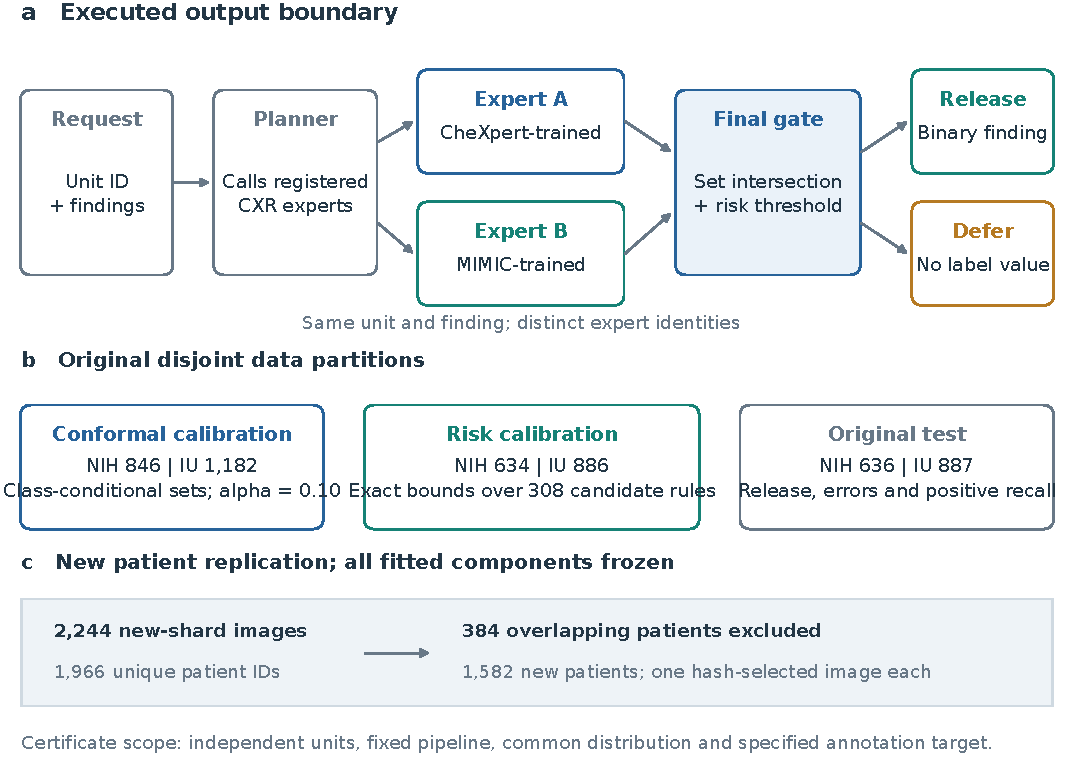
\includegraphics[width=\linewidth]{figures/fig1_architecture.pdf}
\caption{CC-Arbiter's execution path, calibration partitions and new-patient replication. The final gate returns structured binary findings or deferrals. A planner may schedule registered tools, but its free-text response is not the released finding. Both experts must concern the same unit and finding. All original NIH patients, including calibration patients, were excluded from the replication. Fitted models and gates remained frozen.}\label{fig:arch}
\end{figure}

\subsection{Independent calibration of conditional error}
For a fixed finding and threshold $t$, let $A_j(x;t)$ indicate that the proposal is eligible and $u_j(x)\leq t$. The target quantity is
\begin{equation}
R_j(t)=\Pr\{\widehat Y_j\ne\widetilde Y_j\mid A_j(X;t)=1\},
\label{eq:risk}
\end{equation}
when the conditioning event has positive probability. This is distinct from $\Pr\{\widehat Y_j\ne\widetilde Y_j, A_j=1\}$, which can be small solely because release is rare.

The threshold grid $T=\{0,0.05,\ldots,0.50\}$ was fixed before evaluation. For each proposal policy, label and threshold, the independent risk-calibration split yields $N_j(t)$ accepted units and $E_j(t)$ annotation errors. We used the exact one-sided Clopper--Pearson upper bound~\cite{cpinterval}
\begin{equation}
U_j(t)=
\begin{cases}
1, & N_j(t)=0\ \text{or}\ E_j(t)=N_j(t),\\
\operatorname{Beta}^{-1}\!\left(1-\delta/M; E_j(t)+1,N_j(t)-E_j(t)\right), & \text{otherwise},
\end{cases}
\label{eq:bound}
\end{equation}
where $\delta=0.05$ and $M=2\times2\times7\times11=308$ covers the two datasets, two calibrated policies, seven findings and eleven thresholds. For target $r$, the selected threshold is the largest $t$ with $N_j(t)>0$ and $U_j(t)\leq r$. If none qualifies, the finding always defers; zero is not used as a fallback threshold. We evaluated $r\in\{0.05,0.10,0.20\}$ with 0.10 primary. The same simultaneous bounds support all three target choices, so these targets do not create additional threshold families.

Conditional on the independently fitted conformal layer, suppose the risk-calibration and future units are identically distributed and independent. For each fixed candidate rule, the error count conditional on $N_j(t)$ is binomial with parameter $R_j(t)$. The exact upper interval is valid at tail probability $\delta/M$. A union bound gives simultaneous validity for every candidate in the family with probability at least $1-\delta$, allowing selection using the calibration data. Every selected rule then satisfies $R_j(\widehat t_j)\leq r$ on that event. Correlation across labels or experts does not invalidate the union bound; labels are never counted as additional independent binomial trials. The proof is detailed in Additional file~1. Neither monotonic conditional risk nor independence between experts is assumed. The claim is a population bound with calibration confidence, not a per-patient guarantee or a bound on the realized error of every finite test set. For IU, it additionally depends on the unverified independence of reports.

\subsection{Enforced graph execution}
The implemented graph has planning, tool-execution and final-gate nodes (Fig.~\ref{fig:arch}). Methods are registered from the initialized gated class before compilation, avoiding post-compilation class replacement. Evidence is held in invocation state and keyed by request, image or study, finding, and expert identity. Repeated calls overwrite the same expert's evidence; they never count as an additional independent expert. Mismatched image keys, failed calls, nonfinite scores, unsupported tools or missing required findings cannot supply accepted evidence. A failed repeated call invalidates its previous value.

Only the final-gate node creates the returned finding object. Released entries contain binary values; deferred entries contain no finding value and a reason or routing recommendation. A recommendation to obtain another expert or seek review is not evidence that a clinical second pass or human review occurred. We do not certify planner prose, visual question answering, segmentation masks or diagnoses synthesized beyond the seven classifier targets. Thirty-one automated tests, added in three groups as the study was extended, examine statistical edge cases and actual graph behavior, including stale evidence, cross-image mixing, repeated experts, tool failures and attempted planner overrides. The full suite is described in Additional file~1.

We additionally replayed every test unit through the actual LangGraph implementation under two deterministic schedulers: both experts in one round, and one expert per round. Tools returned the newly inferred cached scores without access to reference labels. After the tool calls, each scheduler emitted a deliberate instruction to release every finding as positive. This tested the output boundary rather than language-model reasoning. The designated final object was compared with every offline decision. These replays are software integration evaluations, not end-task LLM accuracy trials or evidence of transfer across agent frameworks.

\subsection{Comparators, outcomes and stress evaluation}
Eight prespecified policies were evaluated on identical test units: always negative; each individual expert at 0.5; mean score at 0.5; agreement of both thresholded experts; conformal singleton intersection without the risk gate; the mean-score risk gate; and CC-Arbiter. With two experts, disagreement is a tie, so the agreement baseline defers rather than fabricating a third vote. The always-negative rule illustrates the effect of class imbalance and was not itself risk-calibrated.

We report release fraction, errors divided by released opportunities, erroneous releases divided by all opportunities, and correctly released positive annotations divided by all positive annotations. The last outcome is positive recall after deferral, so rejected positives count as not recovered. Conditional error is undefined when no predictions are released. Counts are presented by finding, with pooled summaries treated as descriptive. Confidence intervals for pooled quantities use 2,000 bootstrap resamples of independent units, retaining all seven labels together, with seed 718. They condition on the fitted policy; they do not include calibration-set variability. Paired differences use the same resampled units. We make no equivalence or noninferiority claim and did not select thresholds from these intervals.

To test failure mechanisms, a uniform random number was assigned to every test unit with seed 1309. At requested corruption rates of 10\%, 25\% and 50\%, the entire seven-score vector was transformed to $1-p$ for expert B alone, or for both experts with the same mask. The same masks were used across policies, and no case was selected by correctness or reference label. Calibration remained fixed. These experiments model synthetic tool-output failures; the clean-data certificate does not cover the resulting changed score distribution.

\subsection{Secondary comparisons and newly acquired patient replication}
After inspecting the original test results, we fixed a separate, hashed enhancement protocol before acquiring additional NIH data. Analyses on the original test sets are therefore secondary and exploratory. We added two mean-score thresholds per finding: one maximizing Youden's sensitivity plus specificity minus one, and one minimizing empirical classification error. Both used only the original conformal-calibration units, with exact score candidates and ties resolved toward the largest threshold. Neither used risk-calibration or test labels. These baselines have no conditional-risk certificate and do not alter the original family of 308 candidates.

To assess the contribution of rejection, we also matched CC-Arbiter's 10\% policy release count separately for each finding. The alternatives ranked units by distance of their mean score from 0.5 or from the calibration-only Youden threshold, using the corresponding binary prediction. Ties used a hash of unit ID. The resulting batch masks use no reference labels. They are retrospective, cohort-dependent comparisons, not certified deployment policies. Paired bootstrap intervals condition on the fitted thresholds and selected masks. Finding-specific AUROC and average precision (AP), with pointwise 95\% intervals from 2,000 unit bootstrap samples, describe discrimination separately from operating-point performance. Additional file~1 specifies undefined resamples, thresholds and denominators.

We acquired the two prespecified public NIH parquet test shards, numbered 0 and 1, from the \texttt{BahaaEldin0/NIH-Chest-Xray-14} mirror, recording an immutable conversion commit and file hashes. Their 2,244 image records represented 1,966 patients. Excluding all 384 patients shared with the original NIH cohort removed 502 records. Hash-based selection of one image per remaining patient removed 160 additional views, leaving 1,582 patients with no overlap of patient IDs or selected image hashes. Both frozen experts, preprocessing, original NIH conformal quantiles and risk-gate states were reused without refitting. Secondary baseline thresholds also remained fixed. This is newly evaluated, patient-disjoint same-source replication; the data themselves were collected previously. It is not external-center or prospective clinical validation. Certificate transfer still requires a common sampling distribution, which patient disjointness alone cannot establish.

\subsection{Separate positive-sensitive review-routing study}
After the original and replication results were known, a further protocol was locked before acquiring four additional NIH shards. This extension changes the action and estimand: it flags a patient for review rather than releasing a positive diagnosis. Let $Z=1$ denote at least one of the seven annotations, and $F_t=1$ denote a review flag. We separately constrain $\Pr(F_t=0\mid Z=1)$ and $\Pr(Z=1\mid F_t=0)$ to at most 0.10. The former limits missed annotation-positive patients; the latter limits their proportion among unflagged patients. Neither is the original finding-release risk, and an unflagged patient is not declared clinically normal.

Two scores were fixed: a primary logistic stacker of the 14 expert scores, fitted only on the original 846 NIH conformal-calibration patients, and the maximum of the seven expert-mean scores. The additional 4,484 source images represented 3,518 patients. Excluding 961 patients present in either prior NIH cohort and selecting one image per remaining patient yielded 2,557 patients. A fixed random split assigned 1,278 to routing-risk calibration and 1,279 to testing, with no patient or selected-image overlap with previous cohorts. Both one-sided exact binomial bounds use $\delta=0.05$ and a separate family of $2\times41\times2=164$ score--threshold--endpoint combinations. The largest threshold meeting both constraints is selected on calibration only; otherwise all patients are flagged. A distinct final graph node enforces the review action and never supplies a diagnosis value. Additional file~1 specifies fitting, bounds, resampling and execution checks. This is a separate same-source annotation study, not an end-to-end clinical review trial.

\subsection{Use of large language models}
OpenAI Codex was used to revise code, execute the analyses, prepare programmatically generated figures and draft text. It did not generate or adjudicate any reference label, did not determine any released finding, and formed no part of the evaluated system: the released decisions come from the deterministic gate described above. Every reported quantity can be recomputed from the frozen scores in the shared archive, and the authors reviewed and approved the final content.

\section{Results}
\subsection{Coverage and informative evidence}
NIH testing comprised 636 independent patient units and 4,452 label opportunities; IU testing comprised 887 report units and 6,209 opportunities. There were 232 and 193 positive annotation targets, respectively. Across the seven labels, the CheXpert-trained and MIMIC-trained experts had NIH pooled set coverages of 89.1\% and 90.3\%, with mean set sizes of 1.55 and 1.68. IU coverages were 90.1\% and 89.9\%, with mean sizes of 1.77 and 1.73 (Fig.~\ref{fig:coverage}). These pooled quantities do not establish simultaneous or class-wise coverage. Finding-specific denominators and positive/negative coverage are provided in Additional file~1.

Rare classes impose direct limitations on informativeness. For example, only eight IU conformal-calibration reports had a pneumothorax term. At $\alpha=0.10$, the required ninth order statistic is unavailable, so the positive-class threshold becomes infinite. This behavior preserves conservative inclusion of that annotation class, but can prevent a useful negative singleton. Broad sets are therefore an expected consequence of limited calibration support, not evidence that the tool can be safely trusted or that a distribution shift has been detected.

\begin{figure}[htbp]
\centering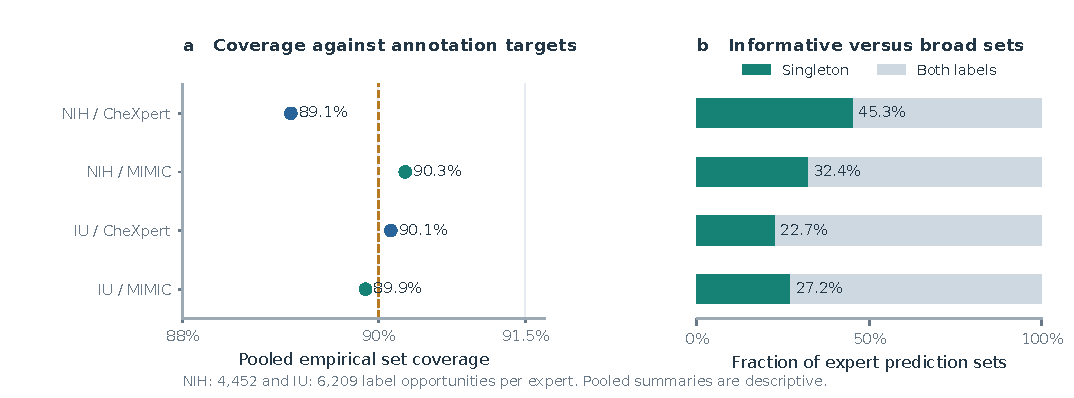
\includegraphics[width=\linewidth]{figures/fig2_coverage.pdf}
\caption{Empirical set coverage and informativeness of the two frozen experts. The dashed vertical line denotes nominal coverage for the class-conditional construction. Pooled coverage is shown descriptively; per-label class counts and coverage are in Additional file~1. There were no empty individual expert sets on these test units. A broad set contains both annotation labels.}\label{fig:coverage}
\end{figure}

\subsection{Selective error and useful release}
At the primary 10\% risk target, CC-Arbiter certified thresholds for three NIH findings: cardiomegaly, consolidation and pneumothorax. The other four findings always deferred. It released 407 of 4,452 opportunities (9.1\%; bootstrap 95\% CI, 8.1--10.2\%), with 10 annotation errors (2.5\% of releases; 95\% CI, 1.1--4.1\%). In comparison, the mean-score risk gate released 1,061 opportunities (23.8\%), with 45 errors (4.2\%). Thus, adding the conformal-intersection requirement reduced both release and erroneous release. The paired decrease in erroneous releases per all opportunities was 0.79 percentage points (95\% CI, 0.54--1.06), accompanied by a 14.69-point decrease in release (95\% CI, 13.93--15.48). This is a rejection trade-off, not evidence of superior diagnostic performance at matched release.

\begin{table}[htbp]
\centering\small\setlength{\tabcolsep}{4pt}
\caption{Primary test results at the 10\% target for the two calibrated gates. Other policies are fixed comparators without this calibration guarantee. TP denotes correctly released positive annotation targets. A dash indicates undefined conditional error.}\label{tab:main}
\begin{tabular}{llrrrr}
\toprule
Dataset & Policy & Release (\%) & Errors / released & Risk (\%) & TP / positives\\
\midrule
NIH & Always negative & 100.0 & 232 / 4452 & 5.2 & 0 / 232\\
NIH & CheXpert expert & 100.0 & 1863 / 4452 & 41.8 & 172 / 232\\
NIH & MIMIC expert & 100.0 & 2599 / 4452 & 58.4 & 201 / 232\\
NIH & Mean score & 100.0 & 1722 / 4452 & 38.7 & 175 / 232\\
NIH & Expert agreement & 70.4 & 1573 / 3136 & 50.2 & 163 / 232\\
NIH & CP intersection & 55.1 & 708 / 2454 & 28.9 & 95 / 232\\
NIH & Risk gate (mean) & 23.8 & 45 / 1061 & 4.2 & 4 / 232\\
NIH & CC-Arbiter & 9.1 & 10 / 407 & 2.5 & 3 / 232\\
\midrule
IU & Always negative & 100.0 & 193 / 6209 & 3.1 & 0 / 193\\
IU & CheXpert expert & 100.0 & 4787 / 6209 & 77.1 & 184 / 193\\
IU & MIMIC expert & 100.0 & 5693 / 6209 & 91.7 & 193 / 193\\
IU & Mean score & 100.0 & 4798 / 6209 & 77.3 & 188 / 193\\
IU & Expert agreement & 78.4 & 4570 / 4869 & 93.9 & 184 / 193\\
IU & CP intersection & 41.0 & 1059 / 2548 & 41.6 & 69 / 193\\
IU & Risk gate (mean) & 5.2 & 7 / 322 & 2.2 & 0 / 193\\
IU & CC-Arbiter & 0.0 & 0 / 0 & -- & 0 / 193\\
\bottomrule
\end{tabular}
\end{table}

On IU, none of the CC-Arbiter candidate thresholds met the required upper bound, and no finding was released. Its observed erroneous-release frequency is zero because all outputs are deferred; its conditional error is undefined. The mean-score gate released 322 of 6,209 opportunities (5.2\%), with seven errors (2.2\% of releases). Figures~\ref{fig:main} and~\ref{fig:cert} show the simultaneous calibration constraints and the resulting coverage of outputs. Increasing the target to 20\% increased NIH CC-Arbiter release to 16.3\%, but IU remained entirely deferred. At the 5\% target, NIH release was 3.1\% with no errors in 137 releases; this observation is not a zero-risk guarantee.

\begin{figure}[htbp]
\centering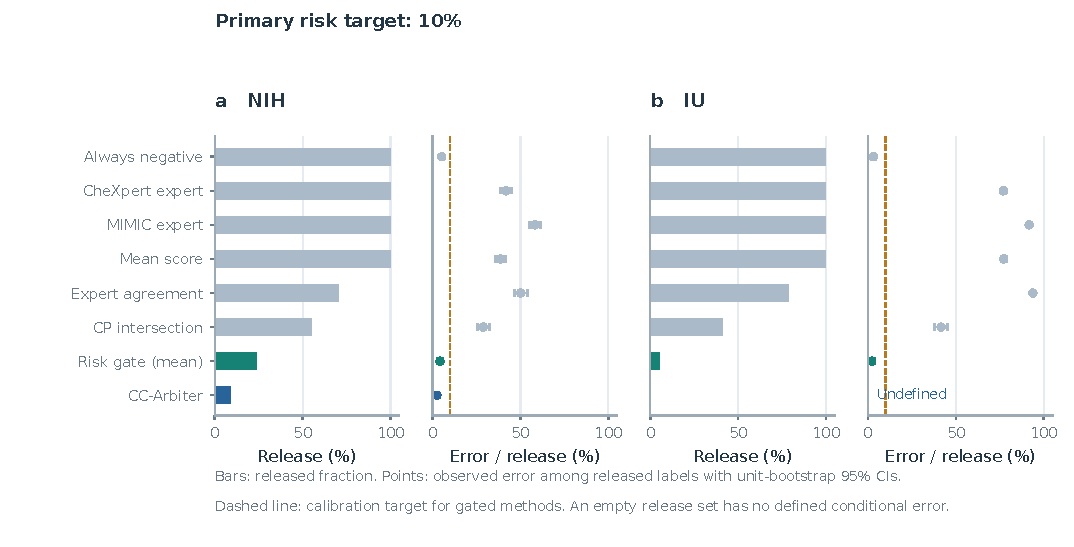
\includegraphics[width=\linewidth]{figures/fig3_selective_performance.pdf}
\caption{Release and empirical conditional error for all prespecified policies. Error intervals resample patients for NIH and reports for IU, keeping correlated labels together. A small error estimate must be interpreted with the associated release fraction and positive retention. The 10\% reference line is the calibration target of the two gated methods; it does not impose a bound on the uncalibrated comparators.}\label{fig:main}
\end{figure}

\begin{figure}[htbp]
\centering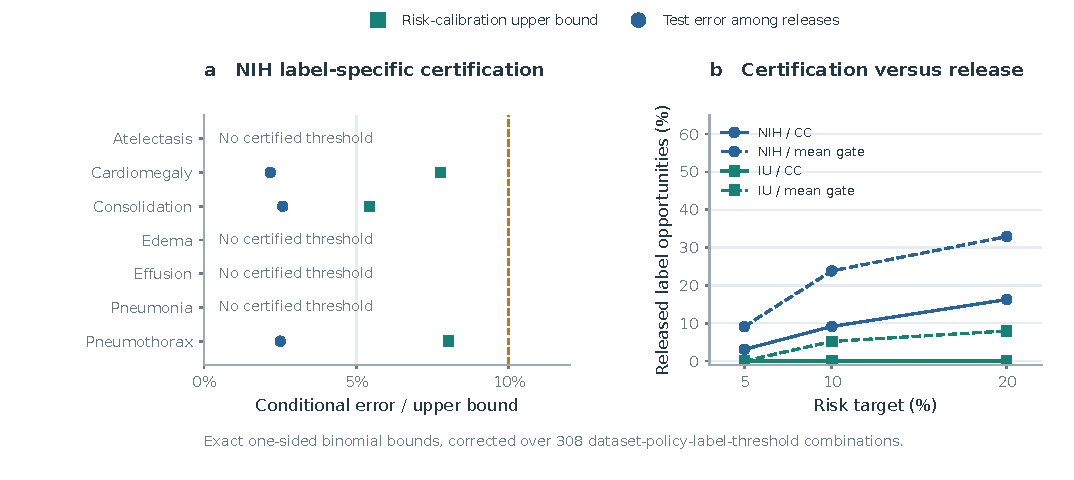
\includegraphics[width=\linewidth]{figures/fig4_risk_certificates.pdf}
\caption{Label-wise certification and its release cost. (a) NIH upper bounds on the independent risk-calibration split and observed test error for the selected CC-Arbiter thresholds. Labels without a qualifying threshold always defer. (b) Released opportunities across the three prespecified targets. Thresholds are selected using calibration only. The IU CC-Arbiter line remains at zero; no conditional-risk estimate is assigned to those empty release sets.}\label{fig:cert}
\end{figure}

The ungated experts and their mean performed poorly against these annotation targets. In particular, mean-score error was 38.7\% on NIH and 77.3\% on IU; simple agreement did not eliminate the high error (Table~\ref{tab:main}). These are properties of the specified released models, normalization, cohort subsets, view aggregation and targets. They should not be generalized to optimized classifiers or to the underlying datasets as a whole.

Class imbalance changes the interpretation of small overall error. An always-negative rule released every opportunity and had empirical error of 5.2\% on NIH and 3.1\% on IU, while recovering no positives. CC-Arbiter correctly released only 3 of 232 NIH positive targets (1.3\%); the mean-score gate recovered 4 (1.7\%). Both recovered no IU positives. Figure~\ref{fig:positive} makes this loss explicit. The observed risk reduction largely reflects withholding outputs and retaining negative annotations. It does not establish a clinically useful screening, triage or diagnostic system.

The low pooled error also did not imply a high positive predictive value. Of CC-Arbiter's eleven positive releases in the original NIH test, three matched the annotation (27.3\%); in the new patients, eight of 26 did (30.8\%). Table~\ref{tab:outcomes} gives the full decomposition of released cells together with the deferred counts. The 232 and 507 positive targets correspond to 172 and 382 patients with at least one positive annotation, so positive-label counts are not independent patient counts.

\begin{table}[htbp]
\centering\small\setlength{\tabcolsep}{5pt}
\caption{CC-Arbiter at the 10\% target, decomposed by released cell and deferral. Counts are label opportunities against the dataset annotations; PPV denotes positive predictive value. Deferred labels receive no finding value.}\label{tab:outcomes}
\begin{tabular}{lrrrrrrrr}
\toprule
Cohort & TP & FP & TN & FN & Deferred positive & Deferred negative & PPV (\%) & Positive recall (\%)\\
\midrule
NIH original test & 3 & 8 & 394 & 2 & 227 & 3,818 & 27.3 & 1.3\\
NIH new patients & 8 & 18 & 1,164 & 5 & 494 & 9,385 & 30.8 & 1.6\\
IU test & 0 & 0 & 0 & 0 & 193 & 6,016 & -- & 0.0\\
\bottomrule
\end{tabular}\par\vspace{3pt}
\noindent\footnotesize TP, FP, TN and FN count released label opportunities only; deferred labels are listed separately and receive no finding value. All comparisons are against the dataset annotations. The dash marks an undefined value when nothing is released.

\end{table}

\begin{figure}[htbp]
\centering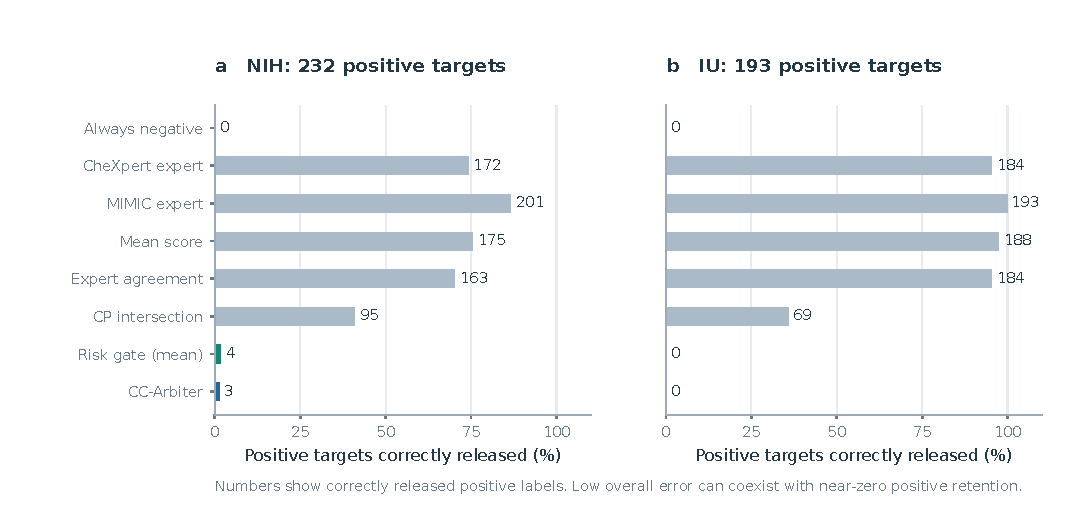
\includegraphics[width=\linewidth]{figures/fig5_positive_retention.pdf}
\caption{Positive annotation targets correctly released after deferral. Numbers next to bars give true-positive counts; the denominators are 232 NIH and 193 IU positive label opportunities. This outcome includes deferral as a failure to recover the positive target. Low pooled conditional error alone can conceal near-total loss of positive findings.}\label{fig:positive}
\end{figure}

\subsection{Correlated failures and execution fidelity}
For NIH, the requested 10\%, 25\% and 50\% masks affected 61, 145 and 325 of 636 patients. With expert B alone flipped, CC-Arbiter released 378, 328 and 238 opportunities, with 10, 10 and 6 errors, respectively. Its released error remained between 2.5\% and 3.0\%, but release decreased. These results are empirical behavior under one corruption mechanism, not an attack guarantee.

Shared corruption had a different effect. Flipping both experts for 61 patients produced 75 errors in 436 released opportunities (17.2\%). At 145 and 325 corrupted patients, error rose to 35.7\% and 62.1\%, respectively (Fig.~\ref{fig:stress}). Correlated incorrect evidence can remain mutually compatible, and clean calibration does not control its changed risk. The experiment therefore rejects a general claim of complete failure containment. IU CC-Arbiter retained its all-defer behavior because it had no certified clean threshold.

\begin{figure}[htbp]
\centering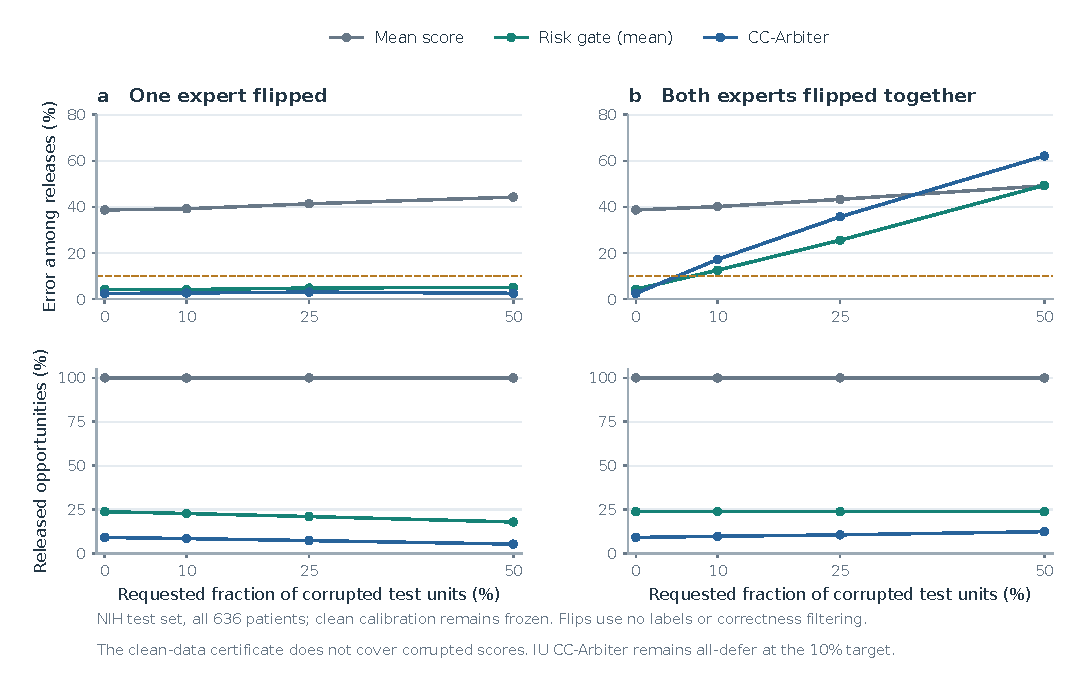
\includegraphics[width=\linewidth]{figures/fig6_correlated_failures.pdf}
\caption{NIH failure stress tests with all patients retained and identical label-independent masks across policies. The horizontal reference is the clean-data calibration target, which is not guaranteed under these corruptions. Unilateral corruption mainly reduces release, whereas shared corruption can generate confident, mutually consistent errors. The score transformation is applied at the tool-output level and does not represent a specific clinical acquisition shift.}\label{fig:stress}
\end{figure}

All 31 original and added automated tests passed. Replaying 3,105 test units, including the new NIH patients, under each of the two scheduling patterns produced 6,210 graph invocations and 43,470 final label decisions, with zero discrepancies against offline CC-Arbiter. Each invocation recorded both distinct expert outputs; deliberately conflicting planner prose did not replace the final structured decisions. Median replay time across cohorts and schedulers was approximately 1.1--2.4 ms per unit, excluding model inference and language-model calls. This verifies the implemented output boundary under the tested conditions, not negligible overhead or clinical accuracy in an end-to-end agent deployment.

\subsection{Secondary operating-point audit and patient replication}
Threshold-free discrimination was better than the poor fixed-threshold errors alone suggest (Fig.~\ref{fig:discrimination}). Mean-score AUROC ranged from 0.672 to 0.839 across findings in the original NIH test, 0.538 to 0.781 in IU, and 0.673 to 0.873 in the new NIH patients. AP and positive denominators are reported in Additional file~1; rare IU targets have especially wide uncertainty. This discrimination does not establish probability calibration or an adequate clinical operating point.

Using only conformal-calibration units to choose Youden thresholds yielded original NIH and IU mean-score errors of 41.5\% and 29.9\%, respectively, recovering 183/232 and 87/193 positive targets at full release. Thus, threshold tuning substantially improved IU performance but did not improve the NIH unweighted error. Thresholds chosen instead to minimize calibration error produced test errors of 5.2\% and 3.2\%, but recovered only two and three positive targets. These opposing outcomes illustrate the importance of defining the utility of positive findings before optimizing a threshold. They also rule out interpreting the original 0.5 baseline as the strongest possible ungated classifier.

\begin{figure}[htbp]
\centering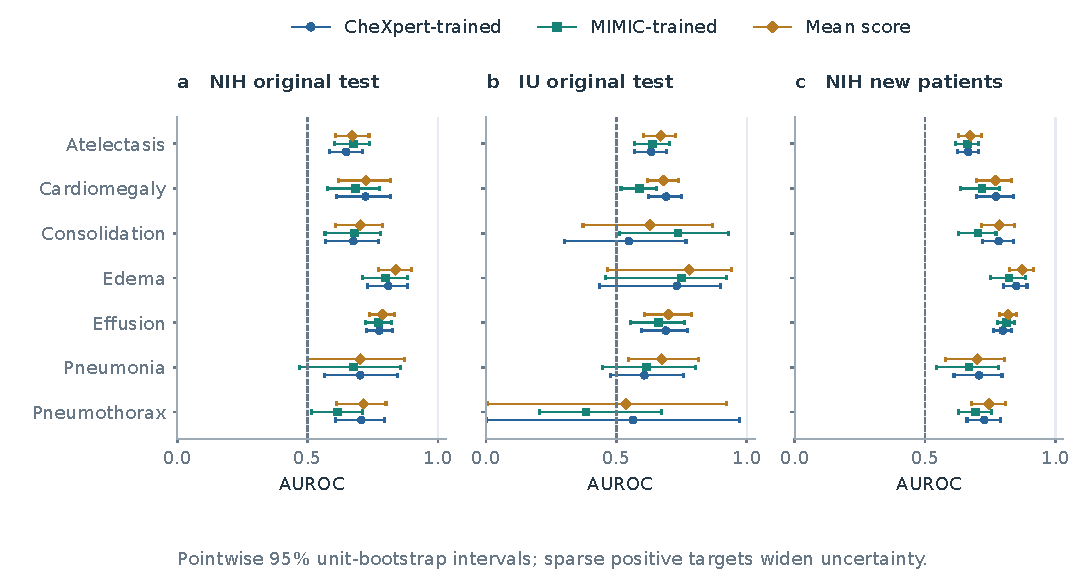
\includegraphics[width=\linewidth]{figures/fig7_discrimination.pdf}
\caption{Secondary audit of discrimination in original and new test cohorts. AUROC and pointwise 95\% intervals use unit bootstrap resampling, preserving within-unit label correlation. Intervals do not correct for comparisons across findings or models and are not used to select a policy. The vertical reference denotes AUROC 0.5. AP, positive counts and valid bootstrap counts are supplied separately.}\label{fig:discrimination}
\end{figure}

The 1,582 new NIH patients contributed 11,074 opportunities and 507 positive targets. Without recalibration, CC-Arbiter released 1,195 opportunities (10.8\%; 95\% CI, 10.1--11.5\%), with 23 errors (1.9\%; 95\% CI, 1.1--2.8\%) and eight positives recovered (1.6\% of positive targets). The mean-score risk gate released 2,949 opportunities with 91 errors and 11 recovered positives (Table~\ref{tab:replication}). The new-patient results reproduce the low-release, low-positive-retention pattern, while remaining subject to the annotation and source-sampling limitations.

\begin{table}[htbp]
\centering\small\setlength{\tabcolsep}{4pt}
\caption{Frozen-policy replication in 1,582 new NIH patients: 11,074 label opportunities and 507 positive targets. TP and recall concern correctly released positive annotations. Gates use the original 10\% target. Matched rules share CC-Arbiter's release count for every finding, use no new target labels for selection and have no risk certificate.}\label{tab:replication}
\begin{tabular}{lrrrrr}\toprule
Policy & Released & Errors & Error (\%) & TP & Recall (\%)\\\midrule
Always negative & 11,074 & 507 & 4.6 & 0 & 0.0 \\
Mean at 0.5 & 11,074 & 3,636 & 32.8 & 377 & 74.4 \\
Mean: calibration Youden & 11,074 & 3,842 & 34.7 & 394 & 77.7 \\
Mean: calibration min. error & 11,074 & 518 & 4.7 & 5 & 1.0 \\
Mean risk gate & 2,949 & 91 & 3.1 & 11 & 2.2 \\
CC-Arbiter & 1,195 & 23 & 1.9 & 8 & 1.6 \\
Mean: matched release & 1,195 & 14 & 1.2 & 3 & 0.6 \\
Youden: matched release & 1,195 & 123 & 10.3 & 25 & 4.9 \\
\bottomrule\end{tabular}

\end{table}

At identical per-label release counts, simple mean-score ranking produced five errors among 407 original NIH releases and 14 among 1,195 new-patient releases, versus CC-Arbiter's 10 and 23 errors (Fig.~\ref{fig:matched}). The CC-minus-ranking conditional-error differences were 1.23 percentage points (paired 95\% CI, 0.28--2.41) and 0.75 points (0.09--1.50), conditional on the fitted thresholds and chosen batch masks. Ranking recovered fewer positives: zero versus three originally, and three versus eight in replication. Youden-based matched ranking recovered more positives (six and 25) but incurred more errors (50 and 123). These are descriptive trade-offs, not a multiplicity-adjusted superiority trial. IU had no nonzero CC-Arbiter release budget, so a matched-release conditional-error comparison was undefined.

\begin{figure}[htbp]
\centering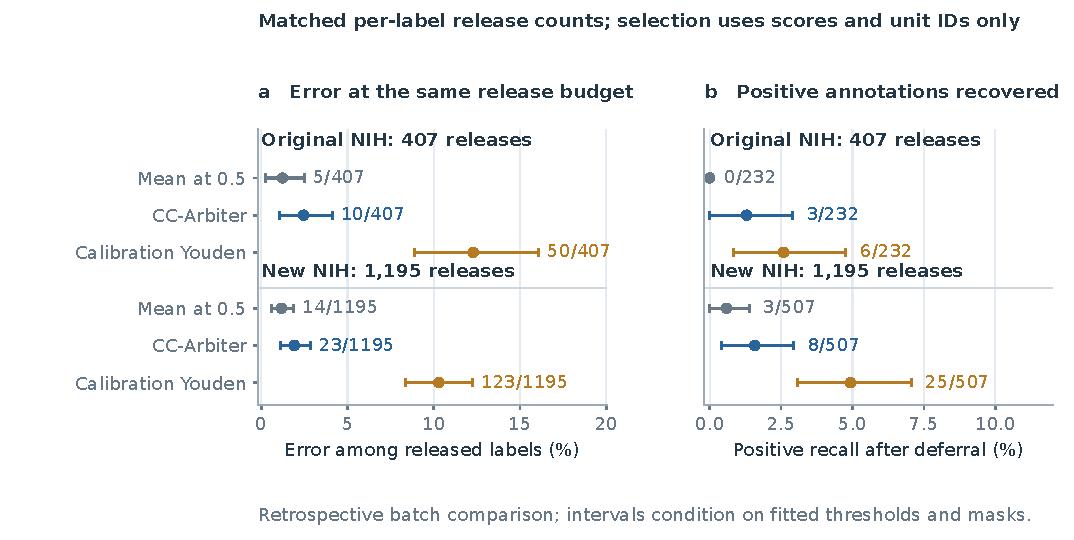
\includegraphics[width=\linewidth]{figures/fig8_matched_replication.pdf}
\caption{Error and positive recall at exactly matched per-finding release counts in two disjoint NIH test cohorts. Mean and Youden ranking select by distance from the corresponding score threshold; ties use a hash of unit ID. Points and intervals use the same patient bootstrap samples, conditional on the observed batch selections. Numerators and denominators are shown explicitly. No comparator uniformly improves both error and positive retention.}\label{fig:matched}
\end{figure}

\subsection{Post hoc projection-stratified audit}
After the primary results were known, we additionally tabulated release, error and positive recovery separately for anteroposterior (AP) and posteroanterior (PA) examinations in both NIH cohorts. Policies, thresholds, calibration states and the reference annotations were unchanged. In the original NIH test, CC-Arbiter released 42 of 1,610 AP opportunities (2.6\%) with seven errors among releases (16.7\%; pointwise patient-bootstrap 95\% CI, 6.3--29.4\%) and 365 of 2,842 PA opportunities (12.8\%) with three errors (0.8\%; 95\% CI, 0.0--1.9\%). The new-patient cohort showed the same ordering: 122 of 3,717 AP opportunities (3.3\%; 5.7\% error; 95\% CI, 1.8--10.1\%) and 1,073 of 7,357 PA opportunities (14.6\%; 1.5\%; 95\% CI, 0.7--2.4\%) (Table~\ref{tab:subgroups}). These analyses were not prespecified and were not adjusted for differences in patient or released-label composition; they carry no projection-specific risk guarantee, and the AP intervals are wide because few labels were released there.

\begin{table}[htbp]
\centering\footnotesize\setlength{\tabcolsep}{3.5pt}
\caption{Post hoc projection-stratified audit in both NIH cohorts with all policies frozen. Intervals are pointwise patient-bootstrap percentile intervals within each stratum and are not multiplicity-adjusted or calibrated as subgroup guarantees.}\label{tab:subgroups}
\begin{tabular}{llrrrrrr}
\toprule
Cohort & Projection & Patients & Released / opportunities & Release (\%) & Errors / released & Error (\%) [95\% CI] & TP / positives\\
\midrule
NIH original test & AP & 230 & 42 / 1,610 & 2.6 & 7 / 42 & 16.7 [6.3, 29.4] & 1 / 102\\
NIH original test & PA & 406 & 365 / 2,842 & 12.8 & 3 / 365 & 0.8 [0.0, 1.9] & 2 / 130\\
NIH new patients & AP & 531 & 122 / 3,717 & 3.3 & 7 / 122 & 5.7 [1.8, 10.1] & 3 / 239\\
NIH new patients & PA & 1,051 & 1,073 / 7,357 & 14.6 & 16 / 1,073 & 1.5 [0.7, 2.4] & 5 / 268\\
\bottomrule
\end{tabular}\par\vspace{3pt}
\noindent\footnotesize Conditional error is undefined for a stratum with no releases; both strata released labels here. Percentile intervals use 2,000 patient bootstrap resamples within each stratum and retain all seven labels per sampled patient.

\end{table}

\subsection{Certification feasibility}
For a candidate with zero observed errors, the exact upper bound is $1-(\delta/M)^{1/n}$. Therefore, at least 171, 83 and 40 accepted risk-calibration units are necessary to certify targets of 5\%, 10\% and 20\%, respectively; any observed errors raise the requirement. These are accepted counts for one fixed candidate, not total cohort sizes or counts pooled across findings. For IU at 10\%, each finding had at least one candidate with 83 or more accepted units, yet no candidate met the error bound. Sample scarcity alone therefore does not explain its all-defer result. Minimum candidate upper bounds ranged from 0.318 to 1.000, compared with 0.046 to 0.239 for NIH. Full counts and bounds are in Additional file~1.

\subsection{Positive attrition and review-routing feasibility}
The original NIH mean-score rule correctly released 175 of 232 positive annotations, the conformal intersection 95, and CC-Arbiter only three (Fig.~\ref{fig:review}a). Moreover, only three of CC-Arbiter's eleven positive releases matched the positive annotation, illustrating that its low pooled error does not imply high positive predictive value. In IU the corresponding correct-positive counts were 188, 69 and zero. The intersection and the risk gate both contribute to positive loss; these summaries do not imply that the intermediate positive sets are nested.

The separate routing-calibration set contained 250 annotation-positive patients. Neither score had a threshold satisfying both 10\% upper bounds (Fig.~\ref{fig:review}b). The minimum upper bound on positivity among unflagged patients was 12.7\% for stacking and 11.6\% for maximum mean, already exceeding the target. Consequently, both selected policies flagged all 1,279 test patients, including all 267 annotation-positive patients. This is the structural all-flag fallback, not an improvement in automatic positive diagnosis, and it reduces no review flags. Fixed 0.5 comparators illustrate the opposing error: the stacker flagged only 73/267 positive patients and maximum mean 216/267, without the specified certificates. Their full counts are in Additional file~1. No actual human reviews or clinical workload savings were measured.

\begin{figure}[htbp]
\centering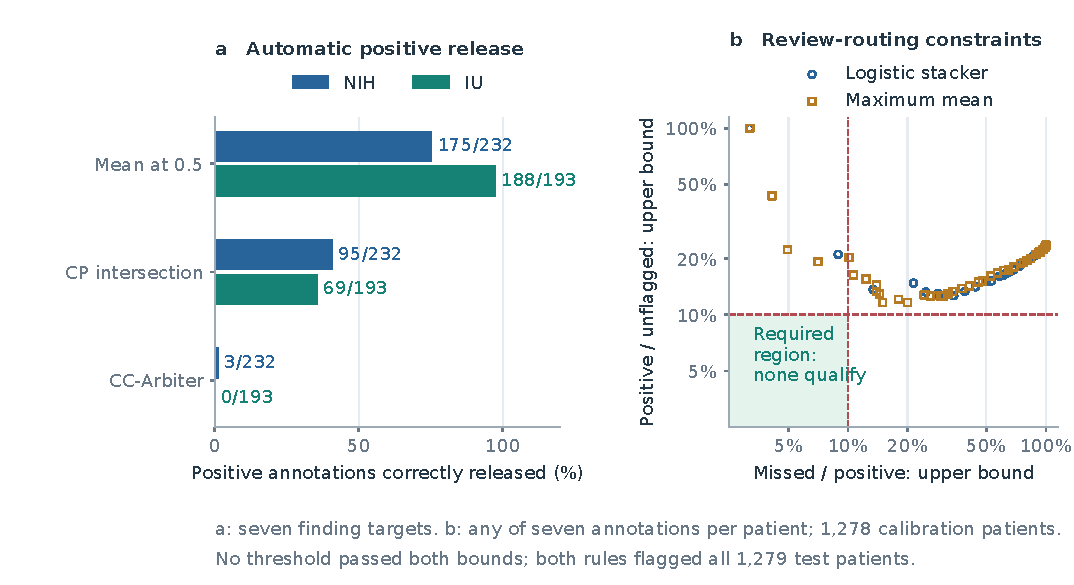
\includegraphics[width=\linewidth]{figures/fig9_positive_review.pdf}
\caption{Positive loss and the feasibility of a separate review action. (a) Correctly released positive annotations in the original tests; the methods are not assumed to form nested positive subsets. (b) Simultaneous exact calibration bounds for 41 thresholds under each of two routing scores. The shaded region requires both bounds at most 10\%; no candidate falls inside it. Axes in panel b are logarithmic. The calibration unit and target differ from panel a: patients with any of seven annotations. All-flag routing does not constitute automatic diagnosis or measured workload reduction.}\label{fig:review}
\end{figure}

\section{Discussion}
This study separates three often conflated properties: calibrated set inclusion, conditional-risk selection, and software enforcement. Individual conformal sets can have coverage close to nominal while their singleton intersection has high selective error. A separately calibrated gate can limit that error while retaining very little evidence. A final graph node can enforce the resulting rule even when the planner proposes a different answer. None of these properties establishes the clinical value of the released findings.

The comparisons with simpler selection are central. Both calibrated gates use the same independent calibration split, candidate thresholds and family correction; the mean-score gate released more labels. At identical per-label budgets, mean-score ranking incurred fewer errors than CC-Arbiter in both NIH cohorts, although it also recovered fewer positives. The conformal-intersection stage is therefore not established as necessary or more efficient. Its role here is to make evidence compatibility explicit. The separately locked new-patient replication strengthens the evidence for this trade-off without converting the secondary original-test analyses into prespecified primary findings.

The all-negative comparator further limits interpretation. With positive annotation rates of only 5.2\% and 3.1\%, unweighted error is an incomplete clinical objective. Our exact bounds control that defined error, but they do not constrain sensitivity, false-negative risk within positive cases, or the clinical cost of missed disease. A system that refuses nearly every positive output cannot be justified by a small pooled error alone. Useful extensions would prespecify class-sensitive losses or simultaneous sensitivity and predictive-value requirements, using enough independently labelled positive cases to calibrate them. Optimizing such requirements after viewing these test results would require a new validation set.

Correlated failure is another boundary. Experts trained on different sources still share an architecture and can fail together. Intersected sets check compatibility rather than truth; they can agree on an incorrect label. We did not assume expert independence in the proof, but the proof does require calibration and future units to follow the same pipeline and distribution. Our corruption changes that distribution. The observed increase to 17.2\% error after joint flips in 9.6\% of NIH patients is therefore consistent with the guarantee's stated domain and shows why it must not be presented as adversarial robustness.

Several limitations affect external validity. The NIH analyses used two original shards, two additional shards for the frozen-policy replication and four further shards for the separate review-routing study, with one hash-selected image per patient throughout. All three patient cohorts were disjoint in the available identifiers and selected-image hashes. They came from the same source, so they do not provide external-centre validation. IU images form a locally available subset, and report-level aggregation includes lateral views. Stable cross-report patient identifiers are unavailable. The secondary threshold audit changes operating points but neither retrains experts nor calibrates their scores as disease probabilities. Label rarity can make conformal thresholds infinite and exact risk bounds conservative, while observed errors can independently prevent certification even when accepted counts are adequate. The study uses text-mined or report-indexing targets without new radiologist adjudication. An error against those targets need not be a clinical error, and agreement need not be clinical correctness. Bootstrap intervals condition on fitted calibration layers and do not capture their sampling variability. Results concern the specified processing and annotation task rather than diagnostic deployment.

Our bounds were calibrated by finding within each data source and were not conditioned on projection, age or the recorded sex field. The post hoc AP/PA differences therefore describe where released outputs occurred rather than a calibrated subgroup guarantee, and they may reflect differences in patient and released-label composition as well as projection-related model behaviour.

The Bonferroni-corrected exact procedure is deliberately simple and can be statistically inefficient. The additional routing study also failed to certify a reduction in review flags under the specified dual objective. It does not prove that all routing scores or calibration methods must fail; it shows that these fixed experts, scores, sample sizes and constraints did not suffice. We did not compare the release efficiency of newer selective-risk methods such as SCoRE~\cite{score}; no optimality claim is made. Deterministic graph replay does not evaluate natural language planning, clinical second-pass resolution or actual human review. Better image-model discrimination, clinically adjudicated targets and independently validated utilities remain necessary before claiming useful clinical performance.

\begin{samepage}
\section{Conclusions}
CC-Arbiter makes finite-sample risk calibration and selective output enforcement jointly auditable. Original and replication NIH cohorts showed low conditional error accompanied by extensive rejection and poor positive retention; IU yielded no certified release. Mean-score ranking had fewer errors at matched release counts but retained fewer positives. A separate positive-sensitive routing study also failed to certify a reduction in review flags, while shared expert corruption defeated clean-data control. The findings support reporting assumptions, execution, release, positive retention and action-specific utility together; they establish neither clinical deployment readiness nor a general accuracy advantage.
\end{samepage}

\section*{Abbreviations}
AP: anteroposterior projection (the ranking metric average precision is written in full); AUROC: area under the receiver operating characteristic curve; CI: confidence interval; FN: false negative; FP: false positive; IU: Indiana University chest radiograph collection; LLM: large language model; MeSH: Medical Subject Headings; NIH: National Institutes of Health ChestX-ray14 collection; PA: posteroanterior projection; PPV: positive predictive value; TF32: TensorFloat-32; TN: true negative; TP: true positive.

\section*{Declarations}
\paragraph{Ethics approval and consent to participate.} This work is a secondary computational analysis of two publicly available, de-identified chest radiograph datasets, NIH ChestX-ray14 and the Indiana University collection. No participants were recruited or contacted, no new clinical data were collected, no intervention was performed and no identifiable information is reported. Because the study uses only previously collected, publicly released, de-identified data, ethics approval and participant consent were not required, and no ethics committee reference number applies. Consent and data-use terms for the original collections were administered by the dataset providers. The authors confirmed this determination with the supervising faculty member (X.~Kong, 12 October 2026).
\paragraph{Consent for publication.} Not applicable. No identifiable individual information or participant images are reproduced in this manuscript.
\paragraph{Availability of data and materials.} The datasets analysed are publicly available and fully cited in the reference list: the NIH ChestX-ray14 collection~\cite{nih} and the Indiana University chest radiograph collection~\cite{iu}. Derived files supporting the conclusions, including the frozen split manifests, expert scores, calibrated thresholds, per-unit decisions and machine-readable results, are included within the article's additional files. Project name: CC-Arbiter reproducibility archive. Project home page: https://github.com/binghe-glacier/cc-arbiter; the same archive accompanies this submission as Additional file~2. Archived version: Zenodo, https://doi.org/10.5281/zenodo.23329663. Operating system: platform independent, developed and tested on Windows~11. Programming language: Python (3.11). Other requirements: NumPy, SciPy and Matplotlib for analysis from the supplied scores; LangGraph and LangChain Core for execution replay; PyTorch and TorchXRayVision for optional re-inference, which additionally requires network access to download public model weights. License: MIT. Restrictions for non-academics: none stated beyond the terms of the source datasets. Original radiographs, report text and pretrained weights are not redistributed and remain subject to their providers' terms.
\paragraph{Competing interests.} The authors declare that they have no competing interests.
\paragraph{Funding.} This research received no specific grant from any funding agency in the public, commercial, or not-for-profit sectors.
\paragraph{Authors' contributions.} YY: Conceptualization, Methodology, Software, Formal analysis, Investigation, Data curation, Visualization, Writing (original draft). XK: Supervision, corresponding author.
\paragraph{Acknowledgements.} Not applicable.

\paragraph{Generative AI assistance.} OpenAI Codex assisted with code revision, execution of the analyses, preparation of programmatically generated figures and manuscript drafting. It produced no reference labels and no released findings. The authors are responsible for verifying and approving the final submitted content.
\paragraph{Additional files.} Additional file~1: supplementary methods, statistical proof, cohort composition, post hoc subgroup descriptives, cohort-level positive counts and detailed calibration results (PDF). Additional file~2: reproducibility archive containing executable code, fixed derived scores, split manifests, machine-readable results and provenance records (ZIP). Original images, report text and model weights are excluded from both files.
\begin{thebibliography}{99}
\small
\bibitem{medrax} Fallahpour A, Ma J, Munim A, Lyu H, Wang B. MedRAX: Medical reasoning agent for chest X-ray. 2025. arXiv:2502.02673.
\bibitem{cxragent} Lou J, Yang Y, Yu Z, Fu Z, Han W, Huang Q, Yu J. CXRAgent: Director-orchestrated multi-stage reasoning for chest X-ray interpretation. 2025. arXiv:2510.21324.
\bibitem{radagents} Zhang K, Barrett CD, Kim J, Sun L, Taghavi T, Kenthapadi K. RadAgents: Multimodal agentic reasoning for chest X-ray interpretation with radiologist-like workflows. MIDL 2026. arXiv:2509.20490.
\bibitem{vovk} Vovk V, Gammerman A, Shafer G. Algorithmic learning in a random world. Springer; 2005.
\bibitem{gentle} Angelopoulos AN, Bates S. A gentle introduction to conformal prediction and distribution-free uncertainty quantification. 2021. arXiv:2107.07511.
\bibitem{ltt} Angelopoulos AN, Bates S, Cand\`es EJ, Jordan MI, Lei L. Learn then test: Calibrating predictive algorithms to achieve risk control. 2021. arXiv:2110.01052.
\bibitem{crc} Angelopoulos AN, Bates S, Fisch A, Lei L, Schuster T. Conformal risk control. ICLR 2024. arXiv:2208.02814.
\bibitem{score} Bai T, Jin Y. Conformal selective prediction with general risk control. 2026. arXiv:2603.24704.
\bibitem{coma} Gasparin M, Ramdas A. Conformal online model aggregation. arXiv:2403.15527. Revised 2025.
\bibitem{nih} Wang X, Peng Y, Lu L, Lu Z, Bagheri M, Summers RM. ChestX-ray8: Hospital-scale chest X-ray database and benchmarks on weakly-supervised classification and localization of common thorax diseases. Proceedings of CVPR. 2017. arXiv:1705.02315.
\bibitem{iu} Demner-Fushman D, Kohli MD, Rosenman MB, et al. Preparing a collection of radiology examinations for distribution and retrieval. J Am Med Inform Assoc. 2016;23:304--310. doi:10.1093/jamia/ocv080.
\bibitem{xrv} Cohen JP, Viviano JD, Bertin P, et al. TorchXRayVision: A library of chest X-ray datasets and models. 2021. arXiv:2111.00595.
\bibitem{densenet} Huang G, Liu Z, van der Maaten L, Weinberger KQ. Densely connected convolutional networks. Proceedings of CVPR. 2017. arXiv:1608.06993.
\bibitem{chex} Irvin J, Rajpurkar P, Ko M, et al. CheXpert: A large chest radiograph dataset with uncertainty labels and expert comparison. 2019. arXiv:1901.07031.
\bibitem{mimic} Johnson AEW, Pollard TJ, Berkowitz SJ, et al. MIMIC-CXR, a de-identified publicly available database of chest radiographs with free-text reports. Sci Data. 2019;6:317. doi:10.1038/s41597-019-0322-0.
\bibitem{cpinterval} Clopper CJ, Pearson ES. The use of confidence or fiducial limits illustrated in the case of the binomial. Biometrika. 1934;26:404--413. doi:10.1093/biomet/26.4.404.
\end{thebibliography}
\end{document}
;
% the compact reading version omits it.
\usepackage{setspace}
\renewcommand{\rmdefault}{ptm}
\renewcommand{\sfdefault}{phv}
\renewcommand{\ttdefault}{phv}
% Font setup that compiles under both engines.
% XeTeX/Tectonic: native OpenType Times/Arial declarations, no extra packages.
% pdfLaTeX (used by the journal's TeX Live 2021 build): standard PS fonts.
\ifdefined\XeTeXversion
\DeclareFontFamily{TU}{ccserif}{}
\DeclareFontShape{TU}{ccserif}{m}{n}{<->"[local-fonts/times.ttf]"}{}
\DeclareFontShape{TU}{ccserif}{m}{it}{<->"[local-fonts/timesi.ttf]"}{}
\DeclareFontShape{TU}{ccserif}{b}{n}{<->"[local-fonts/timesbd.ttf]"}{}
\DeclareFontShape{TU}{ccserif}{bx}{n}{<->"[local-fonts/timesbd.ttf]"}{}
\DeclareFontShape{TU}{ccserif}{b}{it}{<->"[local-fonts/timesbi.ttf]"}{}
\DeclareFontShape{TU}{ccserif}{bx}{it}{<->"[local-fonts/timesbi.ttf]"}{}
\DeclareFontFamily{TU}{ccsans}{}
\DeclareFontShape{TU}{ccsans}{m}{n}{<->"[local-fonts/arial.ttf]"}{}
\DeclareFontShape{TU}{ccsans}{b}{n}{<->"[local-fonts/arialbd.ttf]"}{}
\DeclareFontShape{TU}{ccsans}{bx}{n}{<->"[local-fonts/arialbd.ttf]"}{}
\DeclareFontShape{TU}{ccsans}{m}{it}{<->"[local-fonts/ariali.ttf]"}{}
\renewcommand{\rmdefault}{ccserif}
\renewcommand{\sfdefault}{ccsans}
\renewcommand{\ttdefault}{ccsans}
\else
\usepackage[T1]{fontenc}
\usepackage{mathptmx}
\usepackage[scaled=0.92]{helvet}
\renewcommand{\ttdefault}{phv}
\fi

\DeclareMathSizes{12}{10}{7}{5}
\DeclareMathSizes{9}{10}{7}{5}
\makeatletter\renewcommand\normalsize{\@setfontsize\normalsize{12}{15}}\makeatother
\normalsize
\setlength{\textwidth}{166mm}
\setlength{\textheight}{242mm}
\setlength{\oddsidemargin}{-3mm}
\setlength{\evensidemargin}{-3mm}
\setlength{\topmargin}{-15mm}
\setlength{\parskip}{3pt}
\setlength{\parindent}{12pt}
\setlength{\emergencystretch}{2em}
\renewcommand{\baselinestretch}{1.09}
\ifdefined\REVIEWCOPY\usepackage{lineno}\AtBeginDocument{\doublespacing\linenumbers}\fi
\renewcommand{\topfraction}{0.92}\renewcommand{\bottomfraction}{0.85}
\renewcommand{\textfraction}{0.06}\renewcommand{\floatpagefraction}{0.78}
\title{Auditing selective release of chest radiograph findings: retrospective evaluation of CC-Arbiter}
\author{Yaocong Yang and Xiangyong Kong\\[4pt]
\small School of Health Science and Engineering,\\
\small University of Shanghai for Science and Technology, Shanghai, China\\
\small Correspondence: Xiangyong Kong, \texttt{kxy@usst.edu.cn}}
\date{}
\begin{document}
\maketitle
\begin{abstract}
\noindent\textbf{Background:} Low error among selectively released chest radiograph findings can conceal the rejection of nearly all positive findings. We evaluated an executable evidence gate and audited its release, positive retention and failure boundaries.\par
\noindent\textbf{Methods:} CC-Arbiter intersects class-conditional conformal sets from two frozen DenseNet-121 experts and applies independently calibrated conditional-error gates using exact, multiplicity-corrected binomial bounds. The original cohorts comprised 2,116 NIH patients and 2,955 IU reports, with disjoint conformal, risk-calibration and test splits. Seven dataset annotations served as targets, without new clinical adjudication. A secondary protocol added calibration-only threshold baselines, score discrimination and comparisons at matched release counts. Frozen policies were then evaluated in 1,582 additional NIH patients absent from the original cohort. A separate review-routing study used 2,557 additional NIH patients, split into independent risk-calibration and test sets. It constrained both missed positives and positivity among unflagged patients. Projection-stratified results were examined post hoc. Score corruption and graph execution were also assessed.\par
\noindent\textbf{Results:} At the 10\% risk target, CC-Arbiter released 407/4,452 original NIH opportunities (9.1\%), with 10 errors (2.5\%; unit-bootstrap 95\% confidence interval, 1.1--4.1\%) and only 3/232 positive targets recovered. Positive predictive value was 27.3\%. It released nothing on IU. New-patient replication yielded 1,195/11,074 releases (10.8\%), 23 errors (1.9\%; 95\% confidence interval, 1.1--2.8\%), 8/507 positive targets recovered and positive predictive value of 30.8\%. Anteroposterior examinations received fewer and more erroneous releases than posteroanterior ones (originally 2.6\% versus 12.8\% release; 16.7\% versus 0.8\% error). Simple mean-score ranking at identical per-label release counts produced fewer errors in both NIH cohorts (5 and 14), while recovering fewer positives (0 and 3). Calibration-only Youden thresholds reduced IU mean-score error from 77.3\% to 29.9\%. Shared corruption in 61/636 original NIH patients raised CC-Arbiter error to 17.2\%. Both routing procedures flagged all 1,279 new test patients because no threshold met both constraints. All 43,470 original and replication label decisions matched offline gating.\par
\noindent\textbf{Conclusions:} The framework makes risk calibration and output enforcement auditable, but low selective error did not establish useful positive retention or superiority over simpler selection. Replication supports joint reporting of release, positive recall, matched-budget comparisons and correlated failures.
\end{abstract}
\noindent\textbf{Keywords:} chest radiograph; selective prediction; conformal prediction; risk control; medical imaging agents; reproducibility

\section{Background}
Medical imaging agents combine a planning model with specialist tools for image classification, visual question answering, segmentation and report generation. MedRAX introduced a unified chest radiograph tool interface and the ChestAgentBench benchmark~\cite{medrax}. CXRAgent and RadAgents further develop staged verification and radiologist-inspired workflows~\cite{cxragent,radagents}. These systems motivate a practical engineering question: which tool-derived statements may reach the user when experts disagree or provide uncertain evidence? Providing confidence information to a language model and enforcing an output rule are different operations. A model may disregard an uncertainty annotation, and a correctly written monitor may still be absent from the executed graph.

Conformal prediction provides one component of a solution. Given suitable calibration data and exchangeability, it constructs prediction sets with finite-sample coverage~\cite{vovk,gentle}. Coverage concerns whether a set contains the specified target; it does not by itself bound error among the subset of outputs that a system chooses to release. Intersecting multiple sets, selecting a singleton and withholding some predictions introduce further selection. A separate selective-risk argument is therefore needed. Moreover, a guarantee against imperfect dataset annotations does not become a guarantee against clinical diagnoses.

Risk calibration methods address several different objectives. Learn Then Test calibrates predictive procedures through hypothesis testing~\cite{ltt}. Conformal Risk Control addresses expected bounded losses under its assumptions~\cite{crc}; a joint wrong-and-released loss is not the conditional error among released predictions. SCoRE studies selective risk more directly~\cite{score}. Work on conformal model aggregation also shows that combining prediction sets requires its own analysis~\cite{coma}. Our aim is not to introduce a new conformal theorem. We implement a transparent finite-family procedure whose statistical unit, release rule and software execution can all be checked.

The resulting system, CC-Arbiter, operates on two classifier outputs for the same image or study and finding. It constructs a proposal from intersected conformal sets, calibrates whether that proposal can be released, and replaces the planner's final prose with a structured release-or-defer decision. We evaluate three questions: whether the final gate executes as specified; how much evidence remains after conditional-risk calibration; and whether low overall error is accompanied by useful positive findings or robustness to shared expert failures. The contribution is an auditable implementation and empirical assessment of these questions, including cases where the gate cannot certify useful output.

\section{Methods}
\subsection{Study design and annotation targets}
This retrospective computational study used NIH ChestX-ray14 and IU chest radiograph data~\cite{nih,iu}. The original analysis specification, threshold grid and split manifest were fixed before revised image-model inference and evaluation. This was an internal analysis lock, not public preregistration or a prospectively collected clinical cohort. The pretrained image experts were not fitted on either evaluation dataset. A later, separately specified review-routing extension fits a small score-combination model on original calibration patients only. The primary estimand is error with respect to seven specified dataset annotations: atelectasis, cardiomegaly, consolidation, edema, effusion, pneumonia and pneumothorax.

For NIH, both complete local parquet shards contained 2,458 image records from 2,116 patients. One image per patient was selected using the lexicographically smallest SHA-256 digest of its encoded image bytes, independently of labels and predictions. The resulting 2,116 units contain no duplicated selected image across patient identifiers. We used the released text-mined finding labels, restricted to the seven supported categories. These labels are not newly obtained expert adjudications. The cohort is an available subset of NIH, not the full dataset or an official challenge test set.

For IU, 3,955 XML reports were available; 2,955 had locally available linked PNG images. All linked reports were retained regardless of whether a selected finding was present, including normal reports. Three duplicate image copies within reports were removed, leaving 6,088 distinct report-linked images. Each target is the presence of its prespecified MeSH term in the report's major or minor terms, using the trunk before any slash. For example, \emph{Pleural Effusion} maps to effusion. Absence of a mapped term defines annotation target zero; it is not evidence that the finding is clinically absent. The exact mapping is in Additional file~1. Expert scores were aggregated by their maximum over all available views of a report. This fixed study-level rule includes lateral views and can impair specificity; we did not use outcomes to select a view or aggregation rule. Report identifiers were available, but stable patient identifiers across IU reports were not. Accordingly, patient independence can be enforced for NIH but is only an assumption for IU report-level analyses.

Within each dataset, sorted unit identifiers were shuffled with NumPy's \texttt{default\_rng(20261009)}. The first $\lfloor0.4n\rfloor$ units were assigned to conformal calibration, the next $\lfloor0.3n\rfloor$ to risk calibration, and the remainder to testing (Table~\ref{tab:cohort}). There was no overlap of unit identifiers across splits. All views of an IU report remained together. No image failed the revised inference pipeline. Dataset labels were used only in the appropriate calibration steps or for final scoring, never by the prediction or corruption functions.

\begin{table}[htbp]
\centering\small
\caption{Disjoint calibration and test units. NIH contributes one selected image per patient. IU contributes all available views per report; cross-report patient independence is unverified.}\label{tab:cohort}
\begin{tabular}{llrrrr}
\toprule
Dataset & Unit & Conformal & Risk calibration & Test & Total images\\
\midrule
NIH & Patient & 846 & 634 & 636 & 2,116\\
IU & Report & 1,182 & 886 & 887 & 6,088\\
\bottomrule
\end{tabular}
\end{table}

Table~\ref{tab:characteristics} describes the analysed units, including age, the source dataset's sex field and projection. These descriptors are reported for completeness: the risk bounds were calibrated by finding within each data source and not within demographic or projection strata.

\begin{table}[htbp]
\centering\small\setlength{\tabcolsep}{3.5pt}
\caption{Composition of the analysed cohorts. Source sex is the datasets' recorded Patient Gender field and is not interpreted as biological sex or gender identity. IU report-level descriptors other than image counts and positive targets were not available.}\label{tab:characteristics}
\begin{tabular}{lrrrrrrr}
\toprule
Cohort (unit) & $n$ & Age, median [Q1, Q3] & Range & $<18$ & Source sex (M/F) & AP/PA & Positive targets\\
\midrule
NIH conformal (patient) & 846 & 49 [35, 59] & 2--86 & 47 & 473/373 & 302/544 & 287\\
NIH risk calibration & 634 & 49 [34, 59] & 9--87 & 29 & 361/273 & 220/414 & 178\\
NIH test & 636 & 49 [36, 59] & 2--94 & 23 & 345/291 & 230/406 & 232\\
NIH new replication & 1,582 & 49 [35, 59] & 2--88 & 67 & 898/684 & 531/1,051 & 507\\
NIH routing risk calibration & 1,278 & 48 [34, 58] & 2--82 & 62 & 710/568 & 363/915 & 334\\
NIH routing test & 1,279 & 49 [35, 59] & 3--93 & 61 & 675/604 & 367/912 & 339\\
IU conformal (report) & 1,182 & -- & -- & -- & -- & -- & 283\\
IU risk calibration & 886 & -- & -- & -- & -- & -- & 196\\
IU test & 887 & -- & -- & -- & -- & -- & 193\\
\bottomrule
\end{tabular}\par\vspace{3pt}
\noindent\footnotesize IU images numbered 2,435, 1,827 and 1,826 in the three splits; each NIH patient contributes one selected image. Positive targets are label opportunities and may overlap within a unit. Age quantiles use linear interpolation and are shown as integers.

\end{table}

\subsection{Frozen expert models and preprocessing}
We used TorchXRayVision~\cite{xrv} releases \texttt{densenet121-res224-chex} and \texttt{densenet121-res224-mimic\_ch}. Both use DenseNet-121~\cite{densenet}; their documented training sources are CheXpert~\cite{chex} and MIMIC-CXR~\cite{mimic}, respectively. Thus, the comparison uses different training sources, not different backbone architectures. The selected weight releases do not list NIH or IU as training sources. This source-level audit is not a record-level comparison against the original training databases. Download URLs and SHA-256 weight digests are included with the code.

Each image was decoded to grayscale, normalized to approximately $[-1024,1024]$, centrally cropped, and resized to $224\times224$ with TorchXRayVision's scikit-image resizer. Inference used fixed evaluation-mode models and float32 arithmetic on an NVIDIA RTX 4090, with TF32 disabled. TorchXRayVision's published operating-point normalization was retained. Consequently, the outputs $p_{ej}(x)\in[0,1]$ are model scores, not validated probabilities of disease. Fixed baselines threshold these scores at 0.5. Sixteen randomly selected images were independently rerun one at a time; the maximum absolute deviation from batched scores was below $10^{-6}$. The preprocessing and weight versions were identical across calibration and testing.

\subsection{Conformal evidence and proposal formation}
Let $e\in\{1,2\}$ index experts, $j\in\{1,\ldots,7\}$ index findings, and $\widetilde Y_j\in\{0,1\}$ denote the annotation target. For each expert, finding and target class $c$, the calibration score is $s_{ej}(x,c)=|c-p_{ej}(x)|$. If there are $n_{jc}$ calibration units with $\widetilde Y_j=c$, the threshold is the $\lceil(n_{jc}+1)(1-\alpha)\rceil$-th ordered score. It is $+\infty$ if the required rank exceeds $n_{jc}$, including when that class is absent. We used $\alpha=0.10$ throughout. The class-conditional set is
\begin{equation}
C_{ej}(x)=\{c\in\{0,1\}: |c-p_{ej}(x)|\leq q_{ejc}\}.
\label{eq:sets}
\end{equation}
For a fixed expert and finding, exchangeability within target class gives the usual coverage guarantee for that class~\cite{vovk,gentle}. The guarantee applies to $\widetilde Y_j$, not an unobserved clinical gold standard. It does not assert simultaneous coverage of all findings or experts, nor does it require the empirical test coverage to exceed the nominal level on every finite test set.

We form $I_j(x)=C_{1j}(x)\cap C_{2j}(x)$. If $|I_j(x)|=1$, its sole element is a candidate $\widehat Y_j(x)$; otherwise the finding is ineligible for release. Opposing singleton sets, empty sets, and two broad sets therefore defer. A singleton intersected with a broad set remains a proposal, subject to the risk gate. No expert is selected by comparing the raw magnitude of its nonconformity score with another expert's score. In particular, intersecting two nominal 90\% sets is not claimed to produce another 90\% set or a 10\% selective-error guarantee.

For an eligible proposal, define the scalar uncertainty
\begin{equation}
u_j(x)=\frac12\sum_{e=1}^{2}|\widehat Y_j(x)-p_{ej}(x)|.
\label{eq:uncertainty}
\end{equation}
This is a fixed ranking score rather than a calibrated probability. The mean-score comparator proposes $\mathbf{1}\{(p_{1j}+p_{2j})/2\geq0.5\}$ for every unit and uses the same definition of $u_j$. The two proposal rules are calibrated separately. Changing the expert models, normalization, aggregation or proposal rule would require new calibration.

\begin{figure}[htbp]
\centering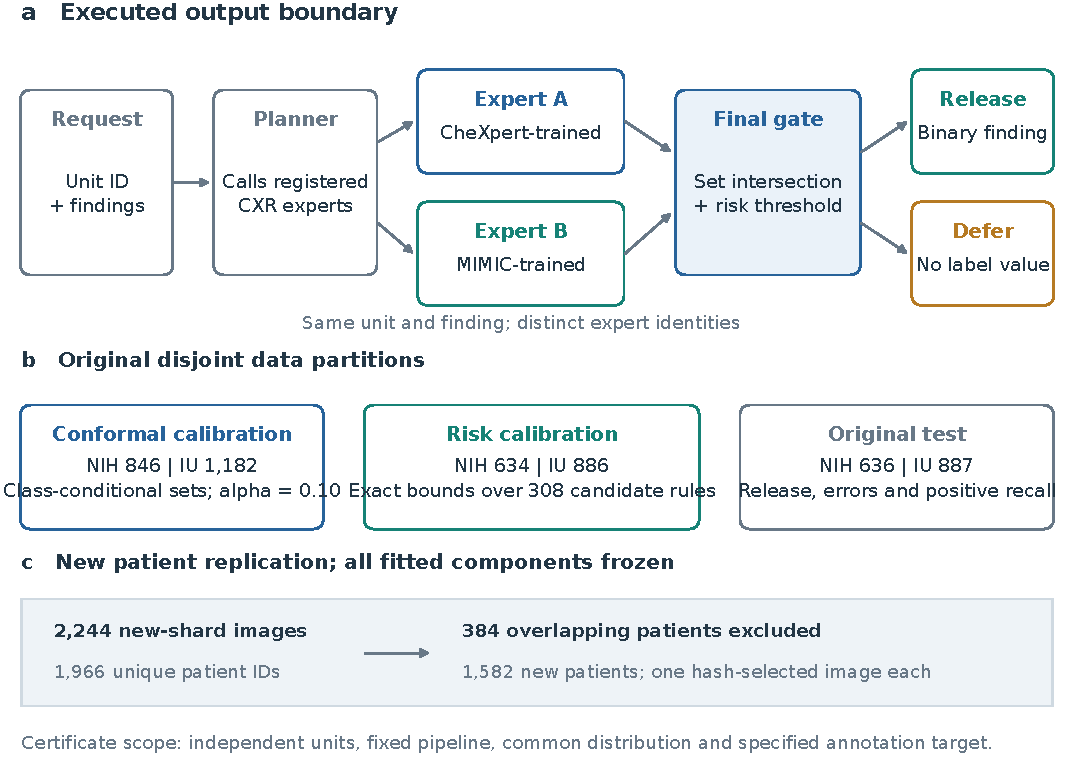
\includegraphics[width=\linewidth]{figures/fig1_architecture.pdf}
\caption{CC-Arbiter's execution path, calibration partitions and new-patient replication. The final gate returns structured binary findings or deferrals. A planner may schedule registered tools, but its free-text response is not the released finding. Both experts must concern the same unit and finding. All original NIH patients, including calibration patients, were excluded from the replication. Fitted models and gates remained frozen.}\label{fig:arch}
\end{figure}

\subsection{Independent calibration of conditional error}
For a fixed finding and threshold $t$, let $A_j(x;t)$ indicate that the proposal is eligible and $u_j(x)\leq t$. The target quantity is
\begin{equation}
R_j(t)=\Pr\{\widehat Y_j\ne\widetilde Y_j\mid A_j(X;t)=1\},
\label{eq:risk}
\end{equation}
when the conditioning event has positive probability. This is distinct from $\Pr\{\widehat Y_j\ne\widetilde Y_j, A_j=1\}$, which can be small solely because release is rare.

The threshold grid $T=\{0,0.05,\ldots,0.50\}$ was fixed before evaluation. For each proposal policy, label and threshold, the independent risk-calibration split yields $N_j(t)$ accepted units and $E_j(t)$ annotation errors. We used the exact one-sided Clopper--Pearson upper bound~\cite{cpinterval}
\begin{equation}
U_j(t)=
\begin{cases}
1, & N_j(t)=0\ \text{or}\ E_j(t)=N_j(t),\\
\operatorname{Beta}^{-1}\!\left(1-\delta/M; E_j(t)+1,N_j(t)-E_j(t)\right), & \text{otherwise},
\end{cases}
\label{eq:bound}
\end{equation}
where $\delta=0.05$ and $M=2\times2\times7\times11=308$ covers the two datasets, two calibrated policies, seven findings and eleven thresholds. For target $r$, the selected threshold is the largest $t$ with $N_j(t)>0$ and $U_j(t)\leq r$. If none qualifies, the finding always defers; zero is not used as a fallback threshold. We evaluated $r\in\{0.05,0.10,0.20\}$ with 0.10 primary. The same simultaneous bounds support all three target choices, so these targets do not create additional threshold families.

Conditional on the independently fitted conformal layer, suppose the risk-calibration and future units are identically distributed and independent. For each fixed candidate rule, the error count conditional on $N_j(t)$ is binomial with parameter $R_j(t)$. The exact upper interval is valid at tail probability $\delta/M$. A union bound gives simultaneous validity for every candidate in the family with probability at least $1-\delta$, allowing selection using the calibration data. Every selected rule then satisfies $R_j(\widehat t_j)\leq r$ on that event. Correlation across labels or experts does not invalidate the union bound; labels are never counted as additional independent binomial trials. The proof is detailed in Additional file~1. Neither monotonic conditional risk nor independence between experts is assumed. The claim is a population bound with calibration confidence, not a per-patient guarantee or a bound on the realized error of every finite test set. For IU, it additionally depends on the unverified independence of reports.

\subsection{Enforced graph execution}
The implemented graph has planning, tool-execution and final-gate nodes (Fig.~\ref{fig:arch}). Methods are registered from the initialized gated class before compilation, avoiding post-compilation class replacement. Evidence is held in invocation state and keyed by request, image or study, finding, and expert identity. Repeated calls overwrite the same expert's evidence; they never count as an additional independent expert. Mismatched image keys, failed calls, nonfinite scores, unsupported tools or missing required findings cannot supply accepted evidence. A failed repeated call invalidates its previous value.

Only the final-gate node creates the returned finding object. Released entries contain binary values; deferred entries contain no finding value and a reason or routing recommendation. A recommendation to obtain another expert or seek review is not evidence that a clinical second pass or human review occurred. We do not certify planner prose, visual question answering, segmentation masks or diagnoses synthesized beyond the seven classifier targets. Thirty-one automated tests, added in three groups as the study was extended, examine statistical edge cases and actual graph behavior, including stale evidence, cross-image mixing, repeated experts, tool failures and attempted planner overrides. The full suite is described in Additional file~1.

We additionally replayed every test unit through the actual LangGraph implementation under two deterministic schedulers: both experts in one round, and one expert per round. Tools returned the newly inferred cached scores without access to reference labels. After the tool calls, each scheduler emitted a deliberate instruction to release every finding as positive. This tested the output boundary rather than language-model reasoning. The designated final object was compared with every offline decision. These replays are software integration evaluations, not end-task LLM accuracy trials or evidence of transfer across agent frameworks.

\subsection{Comparators, outcomes and stress evaluation}
Eight prespecified policies were evaluated on identical test units: always negative; each individual expert at 0.5; mean score at 0.5; agreement of both thresholded experts; conformal singleton intersection without the risk gate; the mean-score risk gate; and CC-Arbiter. With two experts, disagreement is a tie, so the agreement baseline defers rather than fabricating a third vote. The always-negative rule illustrates the effect of class imbalance and was not itself risk-calibrated.

We report release fraction, errors divided by released opportunities, erroneous releases divided by all opportunities, and correctly released positive annotations divided by all positive annotations. The last outcome is positive recall after deferral, so rejected positives count as not recovered. Conditional error is undefined when no predictions are released. Counts are presented by finding, with pooled summaries treated as descriptive. Confidence intervals for pooled quantities use 2,000 bootstrap resamples of independent units, retaining all seven labels together, with seed 718. They condition on the fitted policy; they do not include calibration-set variability. Paired differences use the same resampled units. We make no equivalence or noninferiority claim and did not select thresholds from these intervals.

To test failure mechanisms, a uniform random number was assigned to every test unit with seed 1309. At requested corruption rates of 10\%, 25\% and 50\%, the entire seven-score vector was transformed to $1-p$ for expert B alone, or for both experts with the same mask. The same masks were used across policies, and no case was selected by correctness or reference label. Calibration remained fixed. These experiments model synthetic tool-output failures; the clean-data certificate does not cover the resulting changed score distribution.

\subsection{Secondary comparisons and newly acquired patient replication}
After inspecting the original test results, we fixed a separate, hashed enhancement protocol before acquiring additional NIH data. Analyses on the original test sets are therefore secondary and exploratory. We added two mean-score thresholds per finding: one maximizing Youden's sensitivity plus specificity minus one, and one minimizing empirical classification error. Both used only the original conformal-calibration units, with exact score candidates and ties resolved toward the largest threshold. Neither used risk-calibration or test labels. These baselines have no conditional-risk certificate and do not alter the original family of 308 candidates.

To assess the contribution of rejection, we also matched CC-Arbiter's 10\% policy release count separately for each finding. The alternatives ranked units by distance of their mean score from 0.5 or from the calibration-only Youden threshold, using the corresponding binary prediction. Ties used a hash of unit ID. The resulting batch masks use no reference labels. They are retrospective, cohort-dependent comparisons, not certified deployment policies. Paired bootstrap intervals condition on the fitted thresholds and selected masks. Finding-specific AUROC and average precision (AP), with pointwise 95\% intervals from 2,000 unit bootstrap samples, describe discrimination separately from operating-point performance. Additional file~1 specifies undefined resamples, thresholds and denominators.

We acquired the two prespecified public NIH parquet test shards, numbered 0 and 1, from the \texttt{BahaaEldin0/NIH-Chest-Xray-14} mirror, recording an immutable conversion commit and file hashes. Their 2,244 image records represented 1,966 patients. Excluding all 384 patients shared with the original NIH cohort removed 502 records. Hash-based selection of one image per remaining patient removed 160 additional views, leaving 1,582 patients with no overlap of patient IDs or selected image hashes. Both frozen experts, preprocessing, original NIH conformal quantiles and risk-gate states were reused without refitting. Secondary baseline thresholds also remained fixed. This is newly evaluated, patient-disjoint same-source replication; the data themselves were collected previously. It is not external-center or prospective clinical validation. Certificate transfer still requires a common sampling distribution, which patient disjointness alone cannot establish.

\subsection{Separate positive-sensitive review-routing study}
After the original and replication results were known, a further protocol was locked before acquiring four additional NIH shards. This extension changes the action and estimand: it flags a patient for review rather than releasing a positive diagnosis. Let $Z=1$ denote at least one of the seven annotations, and $F_t=1$ denote a review flag. We separately constrain $\Pr(F_t=0\mid Z=1)$ and $\Pr(Z=1\mid F_t=0)$ to at most 0.10. The former limits missed annotation-positive patients; the latter limits their proportion among unflagged patients. Neither is the original finding-release risk, and an unflagged patient is not declared clinically normal.

Two scores were fixed: a primary logistic stacker of the 14 expert scores, fitted only on the original 846 NIH conformal-calibration patients, and the maximum of the seven expert-mean scores. The additional 4,484 source images represented 3,518 patients. Excluding 961 patients present in either prior NIH cohort and selecting one image per remaining patient yielded 2,557 patients. A fixed random split assigned 1,278 to routing-risk calibration and 1,279 to testing, with no patient or selected-image overlap with previous cohorts. Both one-sided exact binomial bounds use $\delta=0.05$ and a separate family of $2\times41\times2=164$ score--threshold--endpoint combinations. The largest threshold meeting both constraints is selected on calibration only; otherwise all patients are flagged. A distinct final graph node enforces the review action and never supplies a diagnosis value. Additional file~1 specifies fitting, bounds, resampling and execution checks. This is a separate same-source annotation study, not an end-to-end clinical review trial.

\subsection{Use of large language models}
OpenAI Codex was used to revise code, execute the analyses, prepare programmatically generated figures and draft text. It did not generate or adjudicate any reference label, did not determine any released finding, and formed no part of the evaluated system: the released decisions come from the deterministic gate described above. Every reported quantity can be recomputed from the frozen scores in the shared archive, and the authors reviewed and approved the final content.

\section{Results}
\subsection{Coverage and informative evidence}
NIH testing comprised 636 independent patient units and 4,452 label opportunities; IU testing comprised 887 report units and 6,209 opportunities. There were 232 and 193 positive annotation targets, respectively. Across the seven labels, the CheXpert-trained and MIMIC-trained experts had NIH pooled set coverages of 89.1\% and 90.3\%, with mean set sizes of 1.55 and 1.68. IU coverages were 90.1\% and 89.9\%, with mean sizes of 1.77 and 1.73 (Fig.~\ref{fig:coverage}). These pooled quantities do not establish simultaneous or class-wise coverage. Finding-specific denominators and positive/negative coverage are provided in Additional file~1.

Rare classes impose direct limitations on informativeness. For example, only eight IU conformal-calibration reports had a pneumothorax term. At $\alpha=0.10$, the required ninth order statistic is unavailable, so the positive-class threshold becomes infinite. This behavior preserves conservative inclusion of that annotation class, but can prevent a useful negative singleton. Broad sets are therefore an expected consequence of limited calibration support, not evidence that the tool can be safely trusted or that a distribution shift has been detected.

\begin{figure}[htbp]
\centering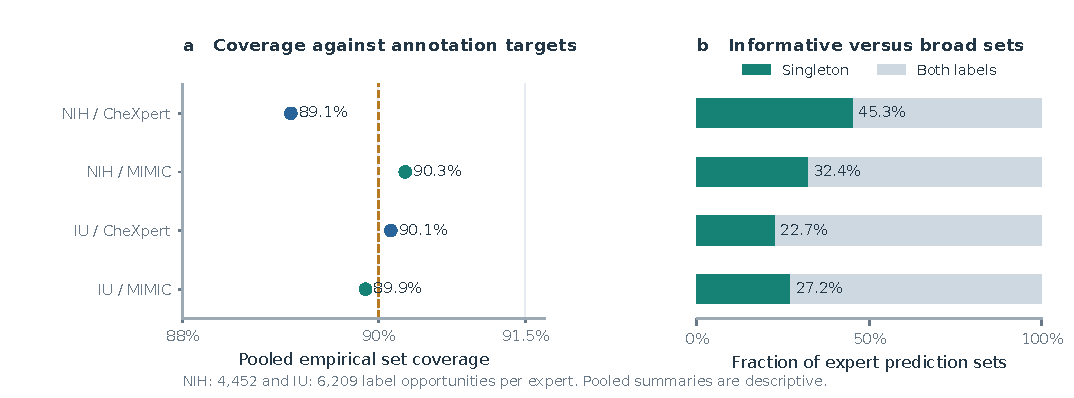
\includegraphics[width=\linewidth]{figures/fig2_coverage.pdf}
\caption{Empirical set coverage and informativeness of the two frozen experts. The dashed vertical line denotes nominal coverage for the class-conditional construction. Pooled coverage is shown descriptively; per-label class counts and coverage are in Additional file~1. There were no empty individual expert sets on these test units. A broad set contains both annotation labels.}\label{fig:coverage}
\end{figure}

\subsection{Selective error and useful release}
At the primary 10\% risk target, CC-Arbiter certified thresholds for three NIH findings: cardiomegaly, consolidation and pneumothorax. The other four findings always deferred. It released 407 of 4,452 opportunities (9.1\%; bootstrap 95\% CI, 8.1--10.2\%), with 10 annotation errors (2.5\% of releases; 95\% CI, 1.1--4.1\%). In comparison, the mean-score risk gate released 1,061 opportunities (23.8\%), with 45 errors (4.2\%). Thus, adding the conformal-intersection requirement reduced both release and erroneous release. The paired decrease in erroneous releases per all opportunities was 0.79 percentage points (95\% CI, 0.54--1.06), accompanied by a 14.69-point decrease in release (95\% CI, 13.93--15.48). This is a rejection trade-off, not evidence of superior diagnostic performance at matched release.

\begin{table}[htbp]
\centering\small\setlength{\tabcolsep}{4pt}
\caption{Primary test results at the 10\% target for the two calibrated gates. Other policies are fixed comparators without this calibration guarantee. TP denotes correctly released positive annotation targets. A dash indicates undefined conditional error.}\label{tab:main}
\begin{tabular}{llrrrr}
\toprule
Dataset & Policy & Release (\%) & Errors / released & Risk (\%) & TP / positives\\
\midrule
NIH & Always negative & 100.0 & 232 / 4452 & 5.2 & 0 / 232\\
NIH & CheXpert expert & 100.0 & 1863 / 4452 & 41.8 & 172 / 232\\
NIH & MIMIC expert & 100.0 & 2599 / 4452 & 58.4 & 201 / 232\\
NIH & Mean score & 100.0 & 1722 / 4452 & 38.7 & 175 / 232\\
NIH & Expert agreement & 70.4 & 1573 / 3136 & 50.2 & 163 / 232\\
NIH & CP intersection & 55.1 & 708 / 2454 & 28.9 & 95 / 232\\
NIH & Risk gate (mean) & 23.8 & 45 / 1061 & 4.2 & 4 / 232\\
NIH & CC-Arbiter & 9.1 & 10 / 407 & 2.5 & 3 / 232\\
\midrule
IU & Always negative & 100.0 & 193 / 6209 & 3.1 & 0 / 193\\
IU & CheXpert expert & 100.0 & 4787 / 6209 & 77.1 & 184 / 193\\
IU & MIMIC expert & 100.0 & 5693 / 6209 & 91.7 & 193 / 193\\
IU & Mean score & 100.0 & 4798 / 6209 & 77.3 & 188 / 193\\
IU & Expert agreement & 78.4 & 4570 / 4869 & 93.9 & 184 / 193\\
IU & CP intersection & 41.0 & 1059 / 2548 & 41.6 & 69 / 193\\
IU & Risk gate (mean) & 5.2 & 7 / 322 & 2.2 & 0 / 193\\
IU & CC-Arbiter & 0.0 & 0 / 0 & -- & 0 / 193\\
\bottomrule
\end{tabular}
\end{table}

On IU, none of the CC-Arbiter candidate thresholds met the required upper bound, and no finding was released. Its observed erroneous-release frequency is zero because all outputs are deferred; its conditional error is undefined. The mean-score gate released 322 of 6,209 opportunities (5.2\%), with seven errors (2.2\% of releases). Figures~\ref{fig:main} and~\ref{fig:cert} show the simultaneous calibration constraints and the resulting coverage of outputs. Increasing the target to 20\% increased NIH CC-Arbiter release to 16.3\%, but IU remained entirely deferred. At the 5\% target, NIH release was 3.1\% with no errors in 137 releases; this observation is not a zero-risk guarantee.

\begin{figure}[htbp]
\centering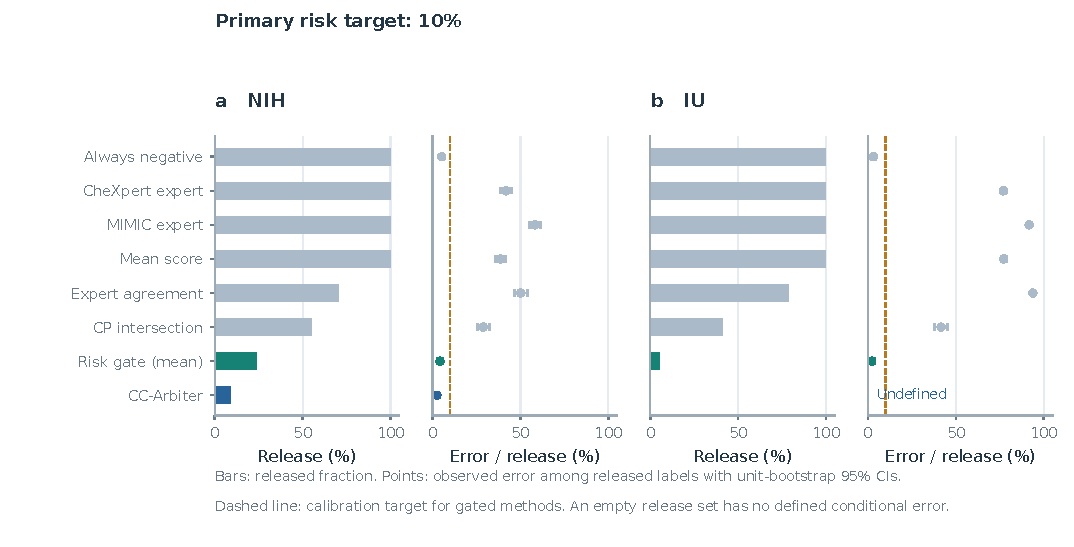
\includegraphics[width=\linewidth]{figures/fig3_selective_performance.pdf}
\caption{Release and empirical conditional error for all prespecified policies. Error intervals resample patients for NIH and reports for IU, keeping correlated labels together. A small error estimate must be interpreted with the associated release fraction and positive retention. The 10\% reference line is the calibration target of the two gated methods; it does not impose a bound on the uncalibrated comparators.}\label{fig:main}
\end{figure}

\begin{figure}[htbp]
\centering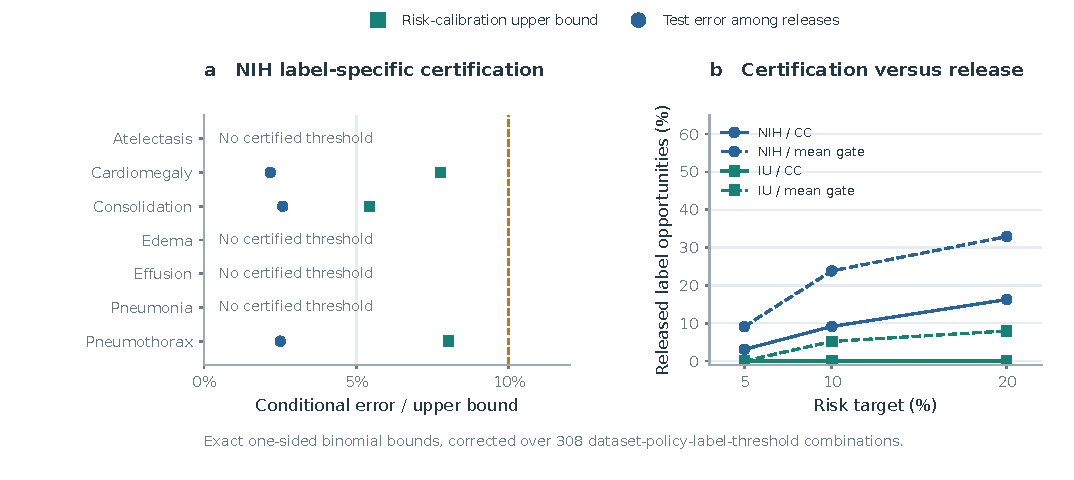
\includegraphics[width=\linewidth]{figures/fig4_risk_certificates.pdf}
\caption{Label-wise certification and its release cost. (a) NIH upper bounds on the independent risk-calibration split and observed test error for the selected CC-Arbiter thresholds. Labels without a qualifying threshold always defer. (b) Released opportunities across the three prespecified targets. Thresholds are selected using calibration only. The IU CC-Arbiter line remains at zero; no conditional-risk estimate is assigned to those empty release sets.}\label{fig:cert}
\end{figure}

The ungated experts and their mean performed poorly against these annotation targets. In particular, mean-score error was 38.7\% on NIH and 77.3\% on IU; simple agreement did not eliminate the high error (Table~\ref{tab:main}). These are properties of the specified released models, normalization, cohort subsets, view aggregation and targets. They should not be generalized to optimized classifiers or to the underlying datasets as a whole.

Class imbalance changes the interpretation of small overall error. An always-negative rule released every opportunity and had empirical error of 5.2\% on NIH and 3.1\% on IU, while recovering no positives. CC-Arbiter correctly released only 3 of 232 NIH positive targets (1.3\%); the mean-score gate recovered 4 (1.7\%). Both recovered no IU positives. Figure~\ref{fig:positive} makes this loss explicit. The observed risk reduction largely reflects withholding outputs and retaining negative annotations. It does not establish a clinically useful screening, triage or diagnostic system.

The low pooled error also did not imply a high positive predictive value. Of CC-Arbiter's eleven positive releases in the original NIH test, three matched the annotation (27.3\%); in the new patients, eight of 26 did (30.8\%). Table~\ref{tab:outcomes} gives the full decomposition of released cells together with the deferred counts. The 232 and 507 positive targets correspond to 172 and 382 patients with at least one positive annotation, so positive-label counts are not independent patient counts.

\begin{table}[htbp]
\centering\small\setlength{\tabcolsep}{5pt}
\caption{CC-Arbiter at the 10\% target, decomposed by released cell and deferral. Counts are label opportunities against the dataset annotations; PPV denotes positive predictive value. Deferred labels receive no finding value.}\label{tab:outcomes}
\begin{tabular}{lrrrrrrrr}
\toprule
Cohort & TP & FP & TN & FN & Deferred positive & Deferred negative & PPV (\%) & Positive recall (\%)\\
\midrule
NIH original test & 3 & 8 & 394 & 2 & 227 & 3,818 & 27.3 & 1.3\\
NIH new patients & 8 & 18 & 1,164 & 5 & 494 & 9,385 & 30.8 & 1.6\\
IU test & 0 & 0 & 0 & 0 & 193 & 6,016 & -- & 0.0\\
\bottomrule
\end{tabular}\par\vspace{3pt}
\noindent\footnotesize TP, FP, TN and FN count released label opportunities only; deferred labels are listed separately and receive no finding value. All comparisons are against the dataset annotations. The dash marks an undefined value when nothing is released.

\end{table}

\begin{figure}[htbp]
\centering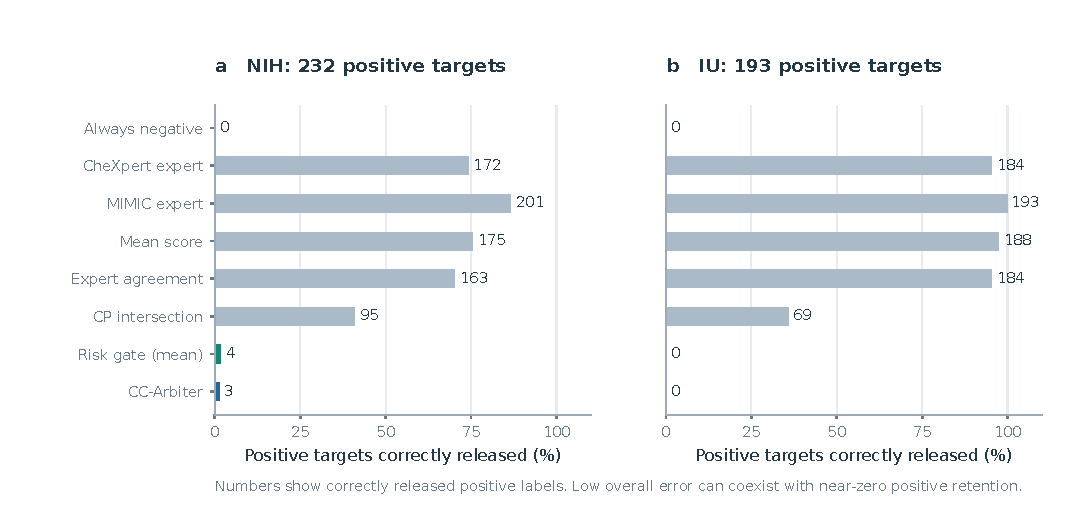
\includegraphics[width=\linewidth]{figures/fig5_positive_retention.pdf}
\caption{Positive annotation targets correctly released after deferral. Numbers next to bars give true-positive counts; the denominators are 232 NIH and 193 IU positive label opportunities. This outcome includes deferral as a failure to recover the positive target. Low pooled conditional error alone can conceal near-total loss of positive findings.}\label{fig:positive}
\end{figure}

\subsection{Correlated failures and execution fidelity}
For NIH, the requested 10\%, 25\% and 50\% masks affected 61, 145 and 325 of 636 patients. With expert B alone flipped, CC-Arbiter released 378, 328 and 238 opportunities, with 10, 10 and 6 errors, respectively. Its released error remained between 2.5\% and 3.0\%, but release decreased. These results are empirical behavior under one corruption mechanism, not an attack guarantee.

Shared corruption had a different effect. Flipping both experts for 61 patients produced 75 errors in 436 released opportunities (17.2\%). At 145 and 325 corrupted patients, error rose to 35.7\% and 62.1\%, respectively (Fig.~\ref{fig:stress}). Correlated incorrect evidence can remain mutually compatible, and clean calibration does not control its changed risk. The experiment therefore rejects a general claim of complete failure containment. IU CC-Arbiter retained its all-defer behavior because it had no certified clean threshold.

\begin{figure}[htbp]
\centering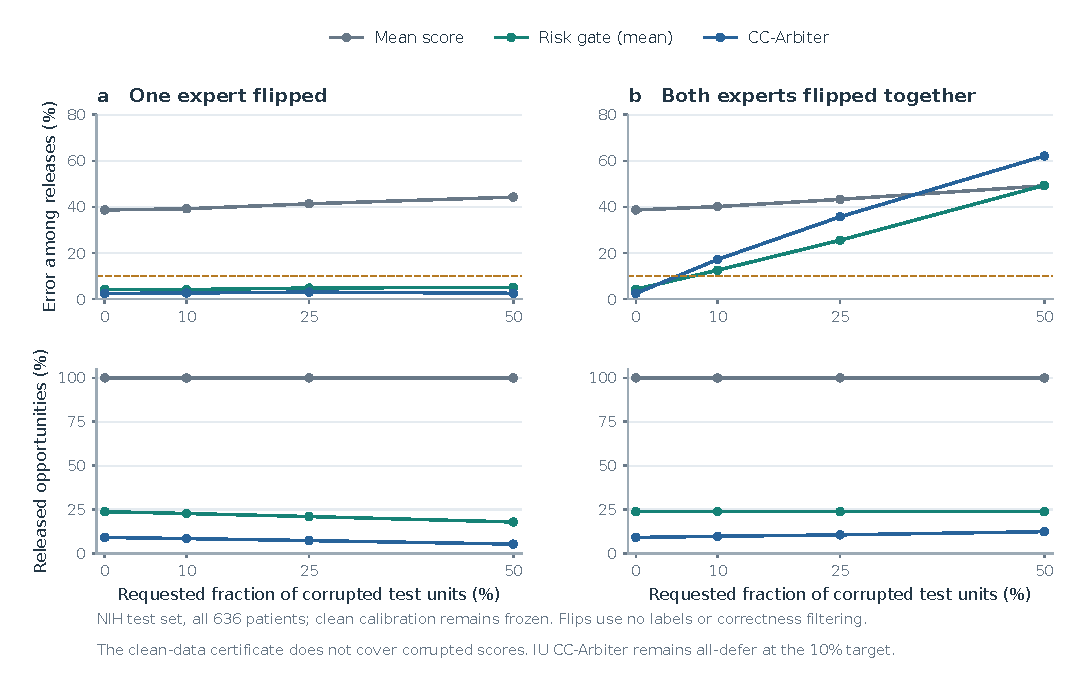
\includegraphics[width=\linewidth]{figures/fig6_correlated_failures.pdf}
\caption{NIH failure stress tests with all patients retained and identical label-independent masks across policies. The horizontal reference is the clean-data calibration target, which is not guaranteed under these corruptions. Unilateral corruption mainly reduces release, whereas shared corruption can generate confident, mutually consistent errors. The score transformation is applied at the tool-output level and does not represent a specific clinical acquisition shift.}\label{fig:stress}
\end{figure}

All 31 original and added automated tests passed. Replaying 3,105 test units, including the new NIH patients, under each of the two scheduling patterns produced 6,210 graph invocations and 43,470 final label decisions, with zero discrepancies against offline CC-Arbiter. Each invocation recorded both distinct expert outputs; deliberately conflicting planner prose did not replace the final structured decisions. Median replay time across cohorts and schedulers was approximately 1.1--2.4 ms per unit, excluding model inference and language-model calls. This verifies the implemented output boundary under the tested conditions, not negligible overhead or clinical accuracy in an end-to-end agent deployment.

\subsection{Secondary operating-point audit and patient replication}
Threshold-free discrimination was better than the poor fixed-threshold errors alone suggest (Fig.~\ref{fig:discrimination}). Mean-score AUROC ranged from 0.672 to 0.839 across findings in the original NIH test, 0.538 to 0.781 in IU, and 0.673 to 0.873 in the new NIH patients. AP and positive denominators are reported in Additional file~1; rare IU targets have especially wide uncertainty. This discrimination does not establish probability calibration or an adequate clinical operating point.

Using only conformal-calibration units to choose Youden thresholds yielded original NIH and IU mean-score errors of 41.5\% and 29.9\%, respectively, recovering 183/232 and 87/193 positive targets at full release. Thus, threshold tuning substantially improved IU performance but did not improve the NIH unweighted error. Thresholds chosen instead to minimize calibration error produced test errors of 5.2\% and 3.2\%, but recovered only two and three positive targets. These opposing outcomes illustrate the importance of defining the utility of positive findings before optimizing a threshold. They also rule out interpreting the original 0.5 baseline as the strongest possible ungated classifier.

\begin{figure}[htbp]
\centering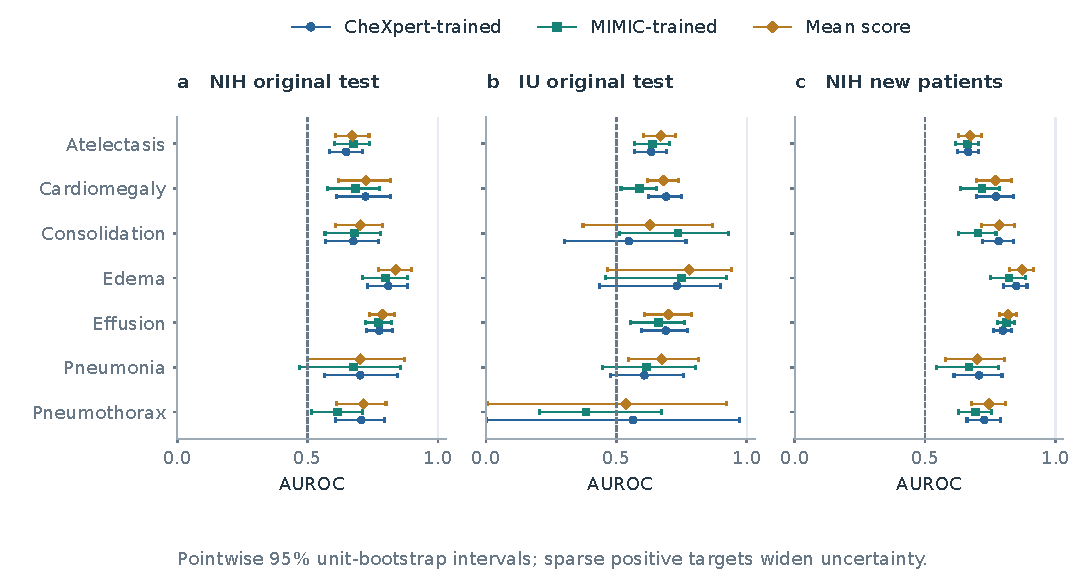
\includegraphics[width=\linewidth]{figures/fig7_discrimination.pdf}
\caption{Secondary audit of discrimination in original and new test cohorts. AUROC and pointwise 95\% intervals use unit bootstrap resampling, preserving within-unit label correlation. Intervals do not correct for comparisons across findings or models and are not used to select a policy. The vertical reference denotes AUROC 0.5. AP, positive counts and valid bootstrap counts are supplied separately.}\label{fig:discrimination}
\end{figure}

The 1,582 new NIH patients contributed 11,074 opportunities and 507 positive targets. Without recalibration, CC-Arbiter released 1,195 opportunities (10.8\%; 95\% CI, 10.1--11.5\%), with 23 errors (1.9\%; 95\% CI, 1.1--2.8\%) and eight positives recovered (1.6\% of positive targets). The mean-score risk gate released 2,949 opportunities with 91 errors and 11 recovered positives (Table~\ref{tab:replication}). The new-patient results reproduce the low-release, low-positive-retention pattern, while remaining subject to the annotation and source-sampling limitations.

\begin{table}[htbp]
\centering\small\setlength{\tabcolsep}{4pt}
\caption{Frozen-policy replication in 1,582 new NIH patients: 11,074 label opportunities and 507 positive targets. TP and recall concern correctly released positive annotations. Gates use the original 10\% target. Matched rules share CC-Arbiter's release count for every finding, use no new target labels for selection and have no risk certificate.}\label{tab:replication}
\begin{tabular}{lrrrrr}\toprule
Policy & Released & Errors & Error (\%) & TP & Recall (\%)\\\midrule
Always negative & 11,074 & 507 & 4.6 & 0 & 0.0 \\
Mean at 0.5 & 11,074 & 3,636 & 32.8 & 377 & 74.4 \\
Mean: calibration Youden & 11,074 & 3,842 & 34.7 & 394 & 77.7 \\
Mean: calibration min. error & 11,074 & 518 & 4.7 & 5 & 1.0 \\
Mean risk gate & 2,949 & 91 & 3.1 & 11 & 2.2 \\
CC-Arbiter & 1,195 & 23 & 1.9 & 8 & 1.6 \\
Mean: matched release & 1,195 & 14 & 1.2 & 3 & 0.6 \\
Youden: matched release & 1,195 & 123 & 10.3 & 25 & 4.9 \\
\bottomrule\end{tabular}

\end{table}

At identical per-label release counts, simple mean-score ranking produced five errors among 407 original NIH releases and 14 among 1,195 new-patient releases, versus CC-Arbiter's 10 and 23 errors (Fig.~\ref{fig:matched}). The CC-minus-ranking conditional-error differences were 1.23 percentage points (paired 95\% CI, 0.28--2.41) and 0.75 points (0.09--1.50), conditional on the fitted thresholds and chosen batch masks. Ranking recovered fewer positives: zero versus three originally, and three versus eight in replication. Youden-based matched ranking recovered more positives (six and 25) but incurred more errors (50 and 123). These are descriptive trade-offs, not a multiplicity-adjusted superiority trial. IU had no nonzero CC-Arbiter release budget, so a matched-release conditional-error comparison was undefined.

\begin{figure}[htbp]
\centering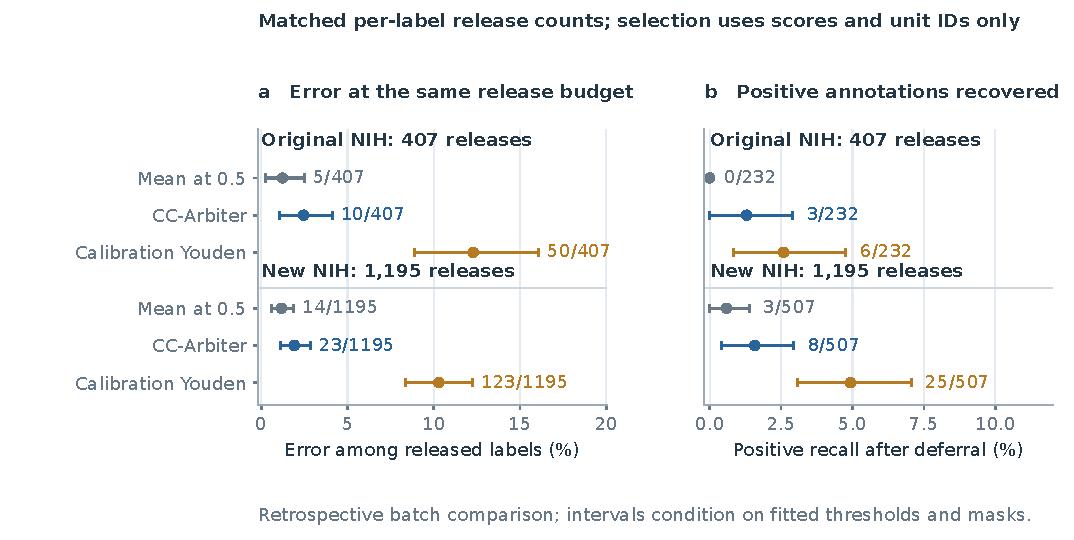
\includegraphics[width=\linewidth]{figures/fig8_matched_replication.pdf}
\caption{Error and positive recall at exactly matched per-finding release counts in two disjoint NIH test cohorts. Mean and Youden ranking select by distance from the corresponding score threshold; ties use a hash of unit ID. Points and intervals use the same patient bootstrap samples, conditional on the observed batch selections. Numerators and denominators are shown explicitly. No comparator uniformly improves both error and positive retention.}\label{fig:matched}
\end{figure}

\subsection{Post hoc projection-stratified audit}
After the primary results were known, we additionally tabulated release, error and positive recovery separately for anteroposterior (AP) and posteroanterior (PA) examinations in both NIH cohorts. Policies, thresholds, calibration states and the reference annotations were unchanged. In the original NIH test, CC-Arbiter released 42 of 1,610 AP opportunities (2.6\%) with seven errors among releases (16.7\%; pointwise patient-bootstrap 95\% CI, 6.3--29.4\%) and 365 of 2,842 PA opportunities (12.8\%) with three errors (0.8\%; 95\% CI, 0.0--1.9\%). The new-patient cohort showed the same ordering: 122 of 3,717 AP opportunities (3.3\%; 5.7\% error; 95\% CI, 1.8--10.1\%) and 1,073 of 7,357 PA opportunities (14.6\%; 1.5\%; 95\% CI, 0.7--2.4\%) (Table~\ref{tab:subgroups}). These analyses were not prespecified and were not adjusted for differences in patient or released-label composition; they carry no projection-specific risk guarantee, and the AP intervals are wide because few labels were released there.

\begin{table}[htbp]
\centering\footnotesize\setlength{\tabcolsep}{3.5pt}
\caption{Post hoc projection-stratified audit in both NIH cohorts with all policies frozen. Intervals are pointwise patient-bootstrap percentile intervals within each stratum and are not multiplicity-adjusted or calibrated as subgroup guarantees.}\label{tab:subgroups}
\begin{tabular}{llrrrrrr}
\toprule
Cohort & Projection & Patients & Released / opportunities & Release (\%) & Errors / released & Error (\%) [95\% CI] & TP / positives\\
\midrule
NIH original test & AP & 230 & 42 / 1,610 & 2.6 & 7 / 42 & 16.7 [6.3, 29.4] & 1 / 102\\
NIH original test & PA & 406 & 365 / 2,842 & 12.8 & 3 / 365 & 0.8 [0.0, 1.9] & 2 / 130\\
NIH new patients & AP & 531 & 122 / 3,717 & 3.3 & 7 / 122 & 5.7 [1.8, 10.1] & 3 / 239\\
NIH new patients & PA & 1,051 & 1,073 / 7,357 & 14.6 & 16 / 1,073 & 1.5 [0.7, 2.4] & 5 / 268\\
\bottomrule
\end{tabular}\par\vspace{3pt}
\noindent\footnotesize Conditional error is undefined for a stratum with no releases; both strata released labels here. Percentile intervals use 2,000 patient bootstrap resamples within each stratum and retain all seven labels per sampled patient.

\end{table}

\subsection{Certification feasibility}
For a candidate with zero observed errors, the exact upper bound is $1-(\delta/M)^{1/n}$. Therefore, at least 171, 83 and 40 accepted risk-calibration units are necessary to certify targets of 5\%, 10\% and 20\%, respectively; any observed errors raise the requirement. These are accepted counts for one fixed candidate, not total cohort sizes or counts pooled across findings. For IU at 10\%, each finding had at least one candidate with 83 or more accepted units, yet no candidate met the error bound. Sample scarcity alone therefore does not explain its all-defer result. Minimum candidate upper bounds ranged from 0.318 to 1.000, compared with 0.046 to 0.239 for NIH. Full counts and bounds are in Additional file~1.

\subsection{Positive attrition and review-routing feasibility}
The original NIH mean-score rule correctly released 175 of 232 positive annotations, the conformal intersection 95, and CC-Arbiter only three (Fig.~\ref{fig:review}a). Moreover, only three of CC-Arbiter's eleven positive releases matched the positive annotation, illustrating that its low pooled error does not imply high positive predictive value. In IU the corresponding correct-positive counts were 188, 69 and zero. The intersection and the risk gate both contribute to positive loss; these summaries do not imply that the intermediate positive sets are nested.

The separate routing-calibration set contained 250 annotation-positive patients. Neither score had a threshold satisfying both 10\% upper bounds (Fig.~\ref{fig:review}b). The minimum upper bound on positivity among unflagged patients was 12.7\% for stacking and 11.6\% for maximum mean, already exceeding the target. Consequently, both selected policies flagged all 1,279 test patients, including all 267 annotation-positive patients. This is the structural all-flag fallback, not an improvement in automatic positive diagnosis, and it reduces no review flags. Fixed 0.5 comparators illustrate the opposing error: the stacker flagged only 73/267 positive patients and maximum mean 216/267, without the specified certificates. Their full counts are in Additional file~1. No actual human reviews or clinical workload savings were measured.

\begin{figure}[htbp]
\centering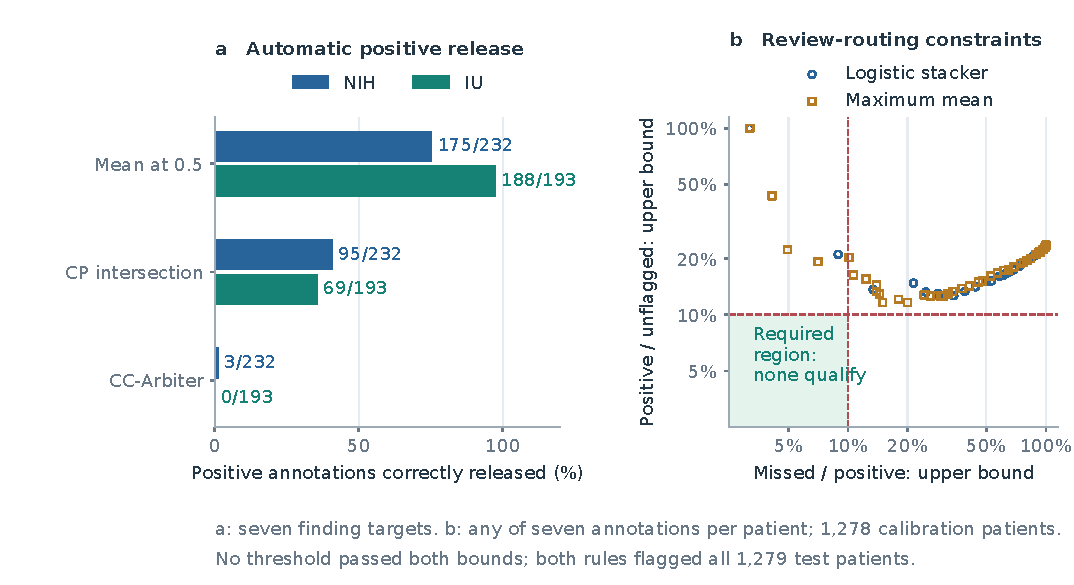
\includegraphics[width=\linewidth]{figures/fig9_positive_review.pdf}
\caption{Positive loss and the feasibility of a separate review action. (a) Correctly released positive annotations in the original tests; the methods are not assumed to form nested positive subsets. (b) Simultaneous exact calibration bounds for 41 thresholds under each of two routing scores. The shaded region requires both bounds at most 10\%; no candidate falls inside it. Axes in panel b are logarithmic. The calibration unit and target differ from panel a: patients with any of seven annotations. All-flag routing does not constitute automatic diagnosis or measured workload reduction.}\label{fig:review}
\end{figure}

\section{Discussion}
This study separates three often conflated properties: calibrated set inclusion, conditional-risk selection, and software enforcement. Individual conformal sets can have coverage close to nominal while their singleton intersection has high selective error. A separately calibrated gate can limit that error while retaining very little evidence. A final graph node can enforce the resulting rule even when the planner proposes a different answer. None of these properties establishes the clinical value of the released findings.

The comparisons with simpler selection are central. Both calibrated gates use the same independent calibration split, candidate thresholds and family correction; the mean-score gate released more labels. At identical per-label budgets, mean-score ranking incurred fewer errors than CC-Arbiter in both NIH cohorts, although it also recovered fewer positives. The conformal-intersection stage is therefore not established as necessary or more efficient. Its role here is to make evidence compatibility explicit. The separately locked new-patient replication strengthens the evidence for this trade-off without converting the secondary original-test analyses into prespecified primary findings.

The all-negative comparator further limits interpretation. With positive annotation rates of only 5.2\% and 3.1\%, unweighted error is an incomplete clinical objective. Our exact bounds control that defined error, but they do not constrain sensitivity, false-negative risk within positive cases, or the clinical cost of missed disease. A system that refuses nearly every positive output cannot be justified by a small pooled error alone. Useful extensions would prespecify class-sensitive losses or simultaneous sensitivity and predictive-value requirements, using enough independently labelled positive cases to calibrate them. Optimizing such requirements after viewing these test results would require a new validation set.

Correlated failure is another boundary. Experts trained on different sources still share an architecture and can fail together. Intersected sets check compatibility rather than truth; they can agree on an incorrect label. We did not assume expert independence in the proof, but the proof does require calibration and future units to follow the same pipeline and distribution. Our corruption changes that distribution. The observed increase to 17.2\% error after joint flips in 9.6\% of NIH patients is therefore consistent with the guarantee's stated domain and shows why it must not be presented as adversarial robustness.

Several limitations affect external validity. The NIH analyses used two original shards, two additional shards for the frozen-policy replication and four further shards for the separate review-routing study, with one hash-selected image per patient throughout. All three patient cohorts were disjoint in the available identifiers and selected-image hashes. They came from the same source, so they do not provide external-centre validation. IU images form a locally available subset, and report-level aggregation includes lateral views. Stable cross-report patient identifiers are unavailable. The secondary threshold audit changes operating points but neither retrains experts nor calibrates their scores as disease probabilities. Label rarity can make conformal thresholds infinite and exact risk bounds conservative, while observed errors can independently prevent certification even when accepted counts are adequate. The study uses text-mined or report-indexing targets without new radiologist adjudication. An error against those targets need not be a clinical error, and agreement need not be clinical correctness. Bootstrap intervals condition on fitted calibration layers and do not capture their sampling variability. Results concern the specified processing and annotation task rather than diagnostic deployment.

Our bounds were calibrated by finding within each data source and were not conditioned on projection, age or the recorded sex field. The post hoc AP/PA differences therefore describe where released outputs occurred rather than a calibrated subgroup guarantee, and they may reflect differences in patient and released-label composition as well as projection-related model behaviour.

The Bonferroni-corrected exact procedure is deliberately simple and can be statistically inefficient. The additional routing study also failed to certify a reduction in review flags under the specified dual objective. It does not prove that all routing scores or calibration methods must fail; it shows that these fixed experts, scores, sample sizes and constraints did not suffice. We did not compare the release efficiency of newer selective-risk methods such as SCoRE~\cite{score}; no optimality claim is made. Deterministic graph replay does not evaluate natural language planning, clinical second-pass resolution or actual human review. Better image-model discrimination, clinically adjudicated targets and independently validated utilities remain necessary before claiming useful clinical performance.

\begin{samepage}
\section{Conclusions}
CC-Arbiter makes finite-sample risk calibration and selective output enforcement jointly auditable. Original and replication NIH cohorts showed low conditional error accompanied by extensive rejection and poor positive retention; IU yielded no certified release. Mean-score ranking had fewer errors at matched release counts but retained fewer positives. A separate positive-sensitive routing study also failed to certify a reduction in review flags, while shared expert corruption defeated clean-data control. The findings support reporting assumptions, execution, release, positive retention and action-specific utility together; they establish neither clinical deployment readiness nor a general accuracy advantage.
\end{samepage}

\section*{Abbreviations}
AP: anteroposterior projection (the ranking metric average precision is written in full); AUROC: area under the receiver operating characteristic curve; CI: confidence interval; FN: false negative; FP: false positive; IU: Indiana University chest radiograph collection; LLM: large language model; MeSH: Medical Subject Headings; NIH: National Institutes of Health ChestX-ray14 collection; PA: posteroanterior projection; PPV: positive predictive value; TF32: TensorFloat-32; TN: true negative; TP: true positive.

\section*{Declarations}
\paragraph{Ethics approval and consent to participate.} This work is a secondary computational analysis of two publicly available, de-identified chest radiograph datasets, NIH ChestX-ray14 and the Indiana University collection. No participants were recruited or contacted, no new clinical data were collected, no intervention was performed and no identifiable information is reported. Because the study uses only previously collected, publicly released, de-identified data, ethics approval and participant consent were not required, and no ethics committee reference number applies. Consent and data-use terms for the original collections were administered by the dataset providers. The authors confirmed this determination with the supervising faculty member (X.~Kong, 12 October 2026).
\paragraph{Consent for publication.} Not applicable. No identifiable individual information or participant images are reproduced in this manuscript.
\paragraph{Availability of data and materials.} The datasets analysed are publicly available and fully cited in the reference list: the NIH ChestX-ray14 collection~\cite{nih} and the Indiana University chest radiograph collection~\cite{iu}. Derived files supporting the conclusions, including the frozen split manifests, expert scores, calibrated thresholds, per-unit decisions and machine-readable results, are included within the article's additional files. Project name: CC-Arbiter reproducibility archive. Project home page: https://github.com/binghe-glacier/cc-arbiter; the same archive accompanies this submission as Additional file~2. Archived version: Zenodo, https://doi.org/10.5281/zenodo.23329663. Operating system: platform independent, developed and tested on Windows~11. Programming language: Python (3.11). Other requirements: NumPy, SciPy and Matplotlib for analysis from the supplied scores; LangGraph and LangChain Core for execution replay; PyTorch and TorchXRayVision for optional re-inference, which additionally requires network access to download public model weights. License: MIT. Restrictions for non-academics: none stated beyond the terms of the source datasets. Original radiographs, report text and pretrained weights are not redistributed and remain subject to their providers' terms.
\paragraph{Competing interests.} The authors declare that they have no competing interests.
\paragraph{Funding.} This research received no specific grant from any funding agency in the public, commercial, or not-for-profit sectors.
\paragraph{Authors' contributions.} YY: Conceptualization, Methodology, Software, Formal analysis, Investigation, Data curation, Visualization, Writing (original draft). XK: Supervision, corresponding author.
\paragraph{Acknowledgements.} Not applicable.

\paragraph{Generative AI assistance.} OpenAI Codex assisted with code revision, execution of the analyses, preparation of programmatically generated figures and manuscript drafting. It produced no reference labels and no released findings. The authors are responsible for verifying and approving the final submitted content.
\paragraph{Additional files.} Additional file~1: supplementary methods, statistical proof, cohort composition, post hoc subgroup descriptives, cohort-level positive counts and detailed calibration results (PDF). Additional file~2: reproducibility archive containing executable code, fixed derived scores, split manifests, machine-readable results and provenance records (ZIP). Original images, report text and model weights are excluded from both files.
\begin{thebibliography}{99}
\small
\bibitem{medrax} Fallahpour A, Ma J, Munim A, Lyu H, Wang B. MedRAX: Medical reasoning agent for chest X-ray. 2025. arXiv:2502.02673.
\bibitem{cxragent} Lou J, Yang Y, Yu Z, Fu Z, Han W, Huang Q, Yu J. CXRAgent: Director-orchestrated multi-stage reasoning for chest X-ray interpretation. 2025. arXiv:2510.21324.
\bibitem{radagents} Zhang K, Barrett CD, Kim J, Sun L, Taghavi T, Kenthapadi K. RadAgents: Multimodal agentic reasoning for chest X-ray interpretation with radiologist-like workflows. MIDL 2026. arXiv:2509.20490.
\bibitem{vovk} Vovk V, Gammerman A, Shafer G. Algorithmic learning in a random world. Springer; 2005.
\bibitem{gentle} Angelopoulos AN, Bates S. A gentle introduction to conformal prediction and distribution-free uncertainty quantification. 2021. arXiv:2107.07511.
\bibitem{ltt} Angelopoulos AN, Bates S, Cand\`es EJ, Jordan MI, Lei L. Learn then test: Calibrating predictive algorithms to achieve risk control. 2021. arXiv:2110.01052.
\bibitem{crc} Angelopoulos AN, Bates S, Fisch A, Lei L, Schuster T. Conformal risk control. ICLR 2024. arXiv:2208.02814.
\bibitem{score} Bai T, Jin Y. Conformal selective prediction with general risk control. 2026. arXiv:2603.24704.
\bibitem{coma} Gasparin M, Ramdas A. Conformal online model aggregation. arXiv:2403.15527. Revised 2025.
\bibitem{nih} Wang X, Peng Y, Lu L, Lu Z, Bagheri M, Summers RM. ChestX-ray8: Hospital-scale chest X-ray database and benchmarks on weakly-supervised classification and localization of common thorax diseases. Proceedings of CVPR. 2017. arXiv:1705.02315.
\bibitem{iu} Demner-Fushman D, Kohli MD, Rosenman MB, et al. Preparing a collection of radiology examinations for distribution and retrieval. J Am Med Inform Assoc. 2016;23:304--310. doi:10.1093/jamia/ocv080.
\bibitem{xrv} Cohen JP, Viviano JD, Bertin P, et al. TorchXRayVision: A library of chest X-ray datasets and models. 2021. arXiv:2111.00595.
\bibitem{densenet} Huang G, Liu Z, van der Maaten L, Weinberger KQ. Densely connected convolutional networks. Proceedings of CVPR. 2017. arXiv:1608.06993.
\bibitem{chex} Irvin J, Rajpurkar P, Ko M, et al. CheXpert: A large chest radiograph dataset with uncertainty labels and expert comparison. 2019. arXiv:1901.07031.
\bibitem{mimic} Johnson AEW, Pollard TJ, Berkowitz SJ, et al. MIMIC-CXR, a de-identified publicly available database of chest radiographs with free-text reports. Sci Data. 2019;6:317. doi:10.1038/s41597-019-0322-0.
\bibitem{cpinterval} Clopper CJ, Pearson ES. The use of confidence or fiducial limits illustrated in the case of the binomial. Biometrika. 1934;26:404--413. doi:10.1093/biomet/26.4.404.
\end{thebibliography}
\end{document}
